\documentclass{article}

\PassOptionsToPackage{numbers,sort&compress}{natbib}
\usepackage[main,final]{neurips_2026}

\usepackage[utf8]{inputenc} % allow utf-8 input
\usepackage[T1]{fontenc}    % use 8-bit T1 fonts
\usepackage{hyperref}       % hyperlinks
\hypersetup{hidelinks}
\usepackage{url}            % simple URL typesetting
\usepackage{booktabs}       % professional-quality tables
\usepackage{amsfonts}       % blackboard math symbols
\usepackage{nicefrac}       % compact symbols for 1/2, etc.
\usepackage{microtype}      % microtypography
\usepackage{xcolor}         % colors

\usepackage{amsthm,amsmath,amssymb}
\usepackage{cleveref}
\usepackage{xspace}
\usepackage{wrapfig}            % For inline figures
\usepackage{placeins}           % For \FloatBarrier
\usepackage{booktabs}           % For \toprule, \midrule, \bottomrule
\usepackage{graphicx}
\usepackage{adjustbox}
\usepackage{mathtools}
\usepackage{subcaption}
\captionsetup[table]{position=top,skip=7pt}
\usepackage{xfrac}
\usepackage{tikz}
\usetikzlibrary{arrows.meta,calc,positioning}

\theoremstyle{plain}
\newtheorem{theorem}{Theorem}
\newtheorem{lemma}{Lemma}
\newtheorem{corollary}{Corollary}
\newtheorem{proposition}{Proposition}


\theoremstyle{definition}
\newtheorem{definition}{Definition}
\newtheorem{assumption}{Assumption}

\theoremstyle{remark}
\newtheorem{remark}{Remark}

\newcommand{\dist}{\Delta}
\newcommand{\N}{\mathbb{N}}
\newcommand{\Z}{\mathbb{Z}}
\newcommand{\Q}{\mathbb{Q}}
\newcommand{\R}{\mathbb{R}}
\newcommand{\C}{\mathbb{C}}
\newcommand{\abs}[1]{\left|#1\right|}
\newcommand{\expectation}{\mathbb{E}}
\newcommand{\momdp}{MO-MDP\xspace}
\newcommand{\momdps}{MO-MDPs\xspace}
\newcommand{\decpomdp}{DEC-POMDP\xspace}
\newcommand{\decpomdps}{DEC-POMDPs\xspace}
\newcommand{\decmdp}{DEC-MDP\xspace}
\newcommand{\decmdps}{DEC-MDPs\xspace}
\newcommand{\mabmdp}{MAB-MDP\xspace}
\renewcommand{\vec}[1]{\mathbf{#1}}
\newcommand{\vecs}{\vec{s}}
\newcommand{\M}{\mathcal{M}}

\newcommand{\richman}{\textsf{Loser-Rewarded}\xspace}
\newcommand{\poorman}{\textsf{Winner-Pays}\xspace}
\newcommand{\allpay}{\textsf{All-Pay}\xspace}

\newcommand{\paths}{\mathit{Paths}}
\renewcommand{\P}{\mathbb{P}}
\newcommand{\E}{\mathbb{E}}
\newcommand{\val}{\mathit{val}}

\newcommand{\slack}{\mathit{slack}}

\newenvironment{nscenter}
 {\parskip=5pt\par\nopagebreak\em\centering}
 {\par\noindent\ignorespacesafterend}
 
\newcommand{\win}{\mathsf{win}}
\newcommand{\wait}{\mathsf{wait}}
\newcommand{\lose}{\mathsf{lose}}
\newcommand{\cont}{\mathsf{cont}}

% comments
\newcommand{\todo}[1]{{\color{orange}\textbf{TODO:} #1}}
\newcommand{\KM}[1]{{\color{red}\textbf{KM:} #1}}
\newcommand{\GS}[1]{{\color{blue}\textbf{GS:} #1}}
% \newcommand{\todo}[1]{}
% \newcommand{\KM}[1]{}
% \newcommand{\GS}[1]{}


% Note. For the workshop paper template, both \title{} and \workshoptitle{} are required, with the former indicating the paper title shown in the title and the latter indicating the workshop title displayed in the footnote. 
\title{Auction-Based Online Policy Adaptation\\for Evolving Objectives}


\author{%
  Guruprerana Shabadi \\
  University of Pennsylvania \\
  United States \\
  \texttt{shabadi@engineering.upenn.edu}
  \And
  Kaushik Mallik \\
  IMDEA Software Institute \\
  Spain \\
  \texttt{kaushik.mallik@imdea.org}
}

\begin{document}


\maketitle



\begin{abstract}
We consider multi-objective reinforcement learning problems where objectives come from an identical family---such as the class of reachability objectives---and may appear or disappear at runtime.
Our goal is to design adaptive policies that can efficiently adjust their behaviors as the set of active objectives changes.
To solve this problem, we propose a modular framework where each objective is supported by a selfish local policy, and coordination is achieved through a novel \emph{auction}-based mechanism:
policies bid for the right to execute their actions, with bids reflecting the urgency of the current state.
The highest bidder selects the action, enabling a dynamic and interpretable trade-off among objectives.
Going back to the original adaptation problem, when objectives change, the system adapts by simply adding or removing the corresponding policies.
Moreover, as objectives arise from the same family, identical copies of a parameterized policy can be deployed, facilitating immediate adaptation at runtime.
We show how the selfish local policies can be computed by turning the problem into a general-sum game, where the policies compete against each other to fulfill their own objectives.
To succeed, each policy must not only optimize its own objective, but also reason about the presence of other goals and learn to produce calibrated bids that reflect relative priority.
Under mild conditions, we prove existence of Nash equilibria that ensure that the most urgent objectives are prioritized.
In our implementation, the policies are trained concurrently using proximal policy optimization (PPO).
We evaluate on two Atari games and a gridworld-based path-planning task with dynamic targets.
Our method achieves substantially better performance than monolithic policies trained with PPO. 
\end{abstract}
\section{Introduction}
\label{sec:introduction}

\newcommand{\introfigleftvoffset}{-3cm}

\begin{wrapfigure}[12]{r}{0.3\textwidth}
  \hspace*{0.6em}\begin{minipage}{\dimexpr\linewidth-1em}
    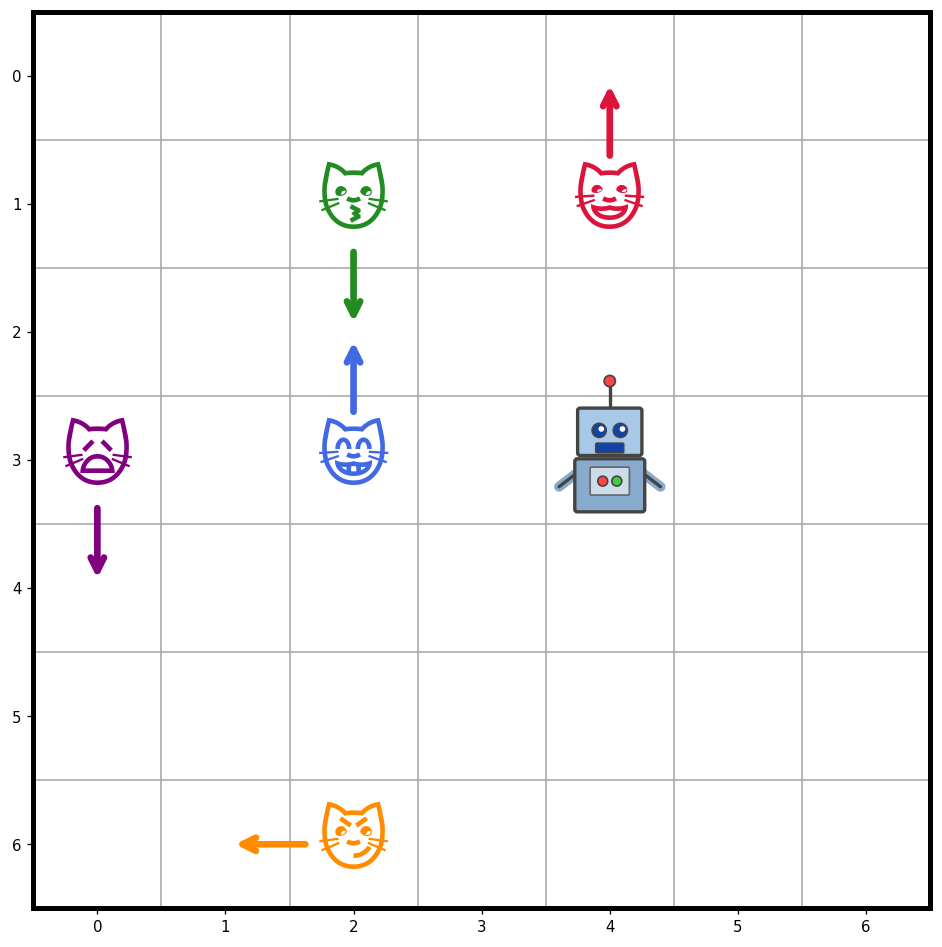
\includegraphics[width=\linewidth]{img/grid_preview.png}
    \caption{Cat Feeder env.}
    \label{fig:grid_preview_intro}
  \end{minipage}
\end{wrapfigure}
Consider the problem of controlling a mobile robot deployed in a cat shelter whose task is to deliver food to cats roaming around the facility (Figure~\ref{fig:grid_preview_intro}). 
New food requests from hungry cats may arrive at arbitrary times and locations, while existing requests may disappear if a cat wanders away before being served.
Since the robot can serve only one cat at a time, fulfilling one request may delay others, potentially allowing some cats to move farther away. 
Thus, the robot must dynamically adapt to the set of active requests to maximize the number of cats fed before they disappear.

In this work, we model the above control problem as a multi-objective reinforcement learning task in which all the objectives come from an identical family, such as reachability in this case.
These objectives can be conflicting and any number of them may be active at a given time.
Moreover, we make no assumptions about their distribution or arrival pattern.
Our goal is to design adaptive policies that update their behavior seamlessly as objectives appear or disappear.

The class of problems we study is relevant to many real-world scenarios.
For example, a warehouse robot must be responsive to changing pickup, delivery, and sorting tasks, and this setting has motivated work on warehouse robot path planning and resource allocation~\citep{chen2023warehouserobot,shen2023amazonrobotics}.
More broadly, such problems have been extensively studied in the planning literature~\citep{fox2006plan}, typically assuming that a precise environment model (like a graph) is available without uncertainties. 
Existing reinforcement learning-based path planning methods~\citep{singh2023reviewrlpathplanning} are able to handle uncertainties but cannot adapt to varying number of objectives at deploying time.
% In contrast, within reinforcement learning (RL) settings---where the environment may be uncertain and a model may not be available---this problem has not been studied to the best of our knowledge.

To solve this problem, we propose a novel compositional RL framework, where each objective is served using a local policy, selfishly maximizing its assigned objective by competing against the other policies.
Coordination between these policies is achieved through a novel auction-based mechanism:
at regular intervals of a given length $\tau>0$, policies submit bids for the right to execute their actions, where bids reflect the urgency of the current state with respect to their objectives. 
The highest bidder selects the action for the next $\tau$ steps, enabling a dynamic and interpretable trade-off among objectives.
Returning to the cat feeder example, suppose the robot approaches an intersection with two active requests, the policy for the first request recommends turning left, while the policy for the second recommends turning right. 
Since both actions cannot be executed simultaneously, a trade-off is unavoidable. 
The auction mechanism determines which objective is prioritized, based on the relative urgency encoded in the bids.

This compositional design yields strong modularity, facilitating fast adaptation:
when an objective appears or disappears, only the corresponding policy needs to be added or removed.
Furthermore, when objectives belong to the identical family---which is reachability in the cat feeder example---a single generalized policy can be trained for the entire family. 
We can deploy identical \emph{copies} of this policy when new objectives arrive, enabling immediate adaptation. 
Modularity also permits us to define objective-specific reward signals while the auction mechanism takes care of the trade-offs between objectives.
For example, we can easily define a distance-based dense reward signal for each policy.
In contrast, in the monolithic case, it is challenging to define such a dense reward signal that strikes the ``optimal'' trade-off between all objectives.
% We have to resort to imposing a preference ordering over the multi-dimensional reward vector, or stick to sparse rewards.
% In contrast, a monolithic policy serving multiple objectives would require additional machinery to impose a dense preference ordering over the multi-dimensional reward vector, which is typically complex and often subject to debate.
We show in our experiments that monolithic policies, trained with both sparse rewards and different types of scalarized dense rewards, achieves significantly lower payoffs as compared to our modular approach.

Yet another advantage of our modular framework is interpretability.
At any moment, we can observe which policy has the control, and thereby the objective currently being pursued by the agent. 
This explanation is beneficial in a range of real-world situations, like providing post-hoc explanations of failures, and also feedback on biases in pursuing different objectives.

We implement our modular framework as a general-sum Markov game between local policies seeking to fulfill their assigned objectives, where each agent's action space is augmented with an additional numeric variable representing the bids.
There are some additional challenges, and below we summarize how we overcome them.

\textbf{Challenge I: Enforcing honest bids.}
The auction mechanism implicitly assumes that the policies would be truthful in selecting their bid values according to the true urgency.
What if policies learn to overbid to suppress competitors?
This would lead to suboptimal results. 
To prevent this, policies are penalized in proportion to their bid values.
As a consequence, excessive bidding reduces the net return of a policy, which is the total accumulated rewards minus the total accumulated bidding penalties. 
Under mild assumptions, we prove that our penalty model implements truthful bidding, i.e., policies would bid high only if the earned rewards outweigh the penalties.


\textbf{Challenge II: Achieving environment awareness.}
Effective bidding not only depends on the current state and the local objective, but also on the  objectives of the competing policies. 
For instance, in the cat feeder problem, if two requests are spatially close, their policies need not compete aggressively. 
Conversely, if requests lie in opposite directions, the urgent policy must bid sufficiently high to win. 
To enable such environment-aware bidding, we allow the policies to observe all the objectives, i.e., the policies have information about the global state. 
But a large number of objectives makes the global state vector very big, resulting in a sluggish training process. 
We equip policies with an \textit{attention pooling} architecture that can extract relevant information from the active objectives into a succinct embedding vector, so that it can be fed as input to the policy.
Each local policy is equipped with its own pooling module which is co-trained with the policy.

% Additionally, the policies are trained concurrently so that they learn to optimize payoffs in the presence of opponents.

\textbf{Challenge III: Variable objective count.}
Recall, we set out to support environments where objectives appear and disappear freely at runtime.
This feature is automatically incorporated by the attention pooling module, which is a learned component with the ability to generalize against different number of competing objectives than the number seen at training time.
Regardless of the objective count, the learned policy always receives a fixed-size encoding of the global state of the environment.

% During deployment, there may be more active objectives than during training. 
% This invalidates standard game-theoretic training formulations which assume a fixed number of opponents. 

We test our framework on three environments with dynamic expected total payoff objectives: the cat feeder environment implemented as a gridworld, and two Atari games: Assault and Air-raid~\citep{bellemare13arcade}.
We use proximal policy optimization (PPO; \cite{schulman2017ppo}) to train each individual policy competing against other policies in the Markov game encoding of the problem.
We report the empirical convergence of the training process, and show that policies trained using our framework exhibit dramatic improvement over the baselines in terms of performance.
We also demonstrate the ability of our approach to generalize to more objectives at test-time than during training.
Lastly, to aid interpretability in renderings of rollouts, we implement visualization of the policy in control and the objective being pursued, through which we get real-time feedback on the strategic behaviors of the policies.

% In summary, our contributions consist of the following:
% \begin{enumerate}
%   \item We formulate an auction-based modular framework for multi-objective RL that consists of objective-specific local policies competing with each other through auctions. Also, theoretical guarantees for urgency-based policy selection are established in~\Cref{sec:auction-framework}.
%   \item We introduce a multi-policy architecture that can handle varying numbers of objectives, and provide a PPO-based training procedure in~\Cref{sec:learning-local-policies}.
%   \item We evaluate the method on three multi-objective environments comparing against baselines in~\Cref{sec:experimental-results} and demonstrate the superior performance of our policies.
% \end{enumerate}

\subsection*{Related Work}

A large body of work in multi-objective reinforcement learning (MORL) relies on \textit{scalarization}, where multiple reward functions are aggregated into a single scalar objective so that standard RL algorithms can be applied. The simplest approach uses weighted sums of rewards~\citep{gass1955computational}, though nonlinear scalarization methods have also been proposed~\citep{van2013scalarized}. A key limitation is that the induced importance among rewards may not reflect the designer’s intent, often leading to a tedious debugging process~\citep{hayes2022practicalguidemorl}. In contrast, our approach achieves a trade-off among reward components without collapsing them into a fixed scalar objective.

Other works address trade-offs by adopting a specific optimality notion, such as Pareto optimality~\citep{van2014multi} and its approximations~\citep{pirotta2015multi}, or fairness-based criteria across rewards~\citep{park2024max,byeon2025multi,siddique2020learning}. These approaches typically learn a single monolithic policy satisfying the chosen criterion. By contrast, we learn independent, selfish policies for each reward component and compose them at runtime, preserving modularity while achieving a coherent global trade-off.

Only a few works consider distributed policies for multiple rewards. W-learning~\citep{humphrys1995w} and its deep RL extension~\citep{rosero2024multi} train separate policies alongside meta-functions that score states by urgency, selecting the policy with the highest score at runtime. Other methods aggregate decisions through ranked voting~\citep{mendez2019multi} or fixed rules such as summing action values~\citep{russell2003q}. Our approach is simpler: it uses an engineered reward structure that enables standard RL algorithms (e.g., PPO) without additional meta-policies or complex aggregation. Moreover, to the best of our knowledge, we are the first to study the incremental MORL setting, where reward components can be added or removed at runtime.

For hierarchical RL, we refer to a recent survey by~\citet{klissarov2025discovering}. 
The similarities between our approach and hierarchical RL are in the desiderata of the design: modularity of design, so that solutions of a given problem can be reused in other problems, and compositionality, where different solutions can be combined to create solutions for a wider range of more complex tasks. 
However the approach is fundamentally different: in hierarchical RL, the above desiderata is achieved by dividing a given learning task to a series of high-level sub-tasks issued by a “manager” with each sub-task being pursued by a lower-level “worker” policy. 
In contrast, we take a “flat”, democratic approach: there is no “manager” and the “workers” still learn to collaborate with each other via a bidding-based conflict-resolution mechanism. 
In the future, it would be interesting to study if these two ideas could be combined into a hybrid architecture.

In multi-policy multi-objective RL~\citep{ding2024multi,zhao2025multi}, each policy represents one point on the Pareto frontier, usually in a way that none of the policies is dominated by some other policy from the collection. 
Then the goal is to pick one of the Pareto optimal policies in a way such that some additional criteria are fulfilled. 
This is fundamentally different from our work: our multiple policies stem from a separation of concern for the objectives, such that each policy pursues a single individual objective. 
In multi-policy MORL, each policy pursues all the objectives simultaneously, which has the same drawbacks as any other monolithic design (lack of reusability, etc., see our introduction).

The idea of bidding-based selfish policies is inspired by auction mechanisms for multi-objective path planning on graphs~\citep{avni2024auction} and by the literature on bidding games~\citep{lazarus1999combinatorial,avni2019infinite,avni2025bidding}. These works use explicit model-based approaches and do not readily extend to the model-free setting of RL.
Besides, they are restricted to the setting with two objectives.



%%% ------- List of all related works collected by Guru --------------------
%\begin{enumerate}
%    \item Fairly comprehensive reference survey of multi-objective RL:~\citet{hayes2022practicalguidemorl}
%    \item Reference for definitions of multi agent RL:~\citet{bucsoniu2010multiagentoverview}.
%    \item W-learning and more recent Deep W learning:~\citet{humphrys1995w,rosero2024multi}
%    \item General multi-objective deep RL works.~\citet{nguyen2020multi} introduce a multi-policy DQN algorithm to learn multiple policies in parallel such that they have access to any possible linear weighting of the objectives. Also has a good lit review from where I got a few of these other citations.
%    \item Multi objective Q learning (tabular):~\citet{van2013scalarized},~\citet{van2014multi} for pareto Q learning (maintains a set of policies and updates them), local search after normal learning:~\citet{van2014novel}
%    \item Use gradient approximation to iteratively build parametrized policies representing pareto frontier~\citet{pirotta2015multi}
%    \item Maximin (fairness) MORL:~\citet{park2024max,byeon2025multi}, fair deep RL:~\citet{siddique2020learning}.
%    \item These two are only vaguely related and look at decomposing an objective into multiple smaller objectives: Q-function decomposition for a single agent with multiple reward components:~\citet{russell2003q} and on a similar note hybrid reward architecture:~\citet{van2017hybrid}
%\end{enumerate}
%%% --------------------------------------------------------------------------

%\section{Preliminaries: Multi-Objective MDPs}
\label{sec:preliminaries}

Mainstream RL algorithms consider Markov decision processes (MDP) equipped with a \textit{single} reward function, pertaining to a single task or \textit{objective} for the system.
In reality, a majority of real-world applications of RL requires satisfying multiple, partly contradictory objectives.
We model such multi-objective decision-making problems using multi-objective MDPs (MO-MDP), as formally defined below.
Intuitively, an MO-MDP has the exact same syntax as a regular MDP, except that it now has multiple reward functions pertaining to the different objectives.
We formalize \momdp below.
We will use the notation $\dist(\Sigma)$ to represent the set of all probability distributions over a given alphabet $\Sigma$.

\begin{definition}[\momdp]\label{def:MO-MDP}
    A multi-objective Markov decision process (\momdp) with \(m \in \Z_{>0}\) objectives is specified by a tuple \(\mathcal{M} = (S, A, T, \mathbf{R}, \mu_0)\), where
    \begin{itemize}
        \item \(S\) is the set of states,
        \item \(A\) is the set of actions,
        \item \(T : S \times A \to \dist(S)\) is the transition function mapping a state-action pair to a distribution over the successor states,
        \item \(\mathbf{R}=\{R^i : S \times A \times S \to \R_{\geq 0}\}_{i\in [1;m]}\) is the set of reward functions, and
        \item \(\mu_0 \in \dist(S)\) is the initial state distribution.
    \end{itemize}
\end{definition}

The notions of policies and paths induced by them are exactly the same as in classical MDPs, which we briefly recall below.
First, we introduce some notation.
Given an alphabet $\Sigma$, we will write $\Sigma^*$ and $\Sigma^\omega$ to denote the set of every finite and infinite word over $\Sigma$, respectively, and will write $\Sigma^\infty = \Sigma^*\cup \Sigma^\omega$.
Given a word $w = \sigma_0\sigma_1\ldots\in \Sigma^\infty$, and given a $t\geq 0$ that is not larger than the length of $w$, we will write $w_t$ and $w_{0:t}$ to denote respectively the $t$-th element of $w$, i.e., $w_t=\sigma_t$, and the prefix of $w$ up to the $t$-th element, i.e., $w_{0:t} = \sigma_0\ldots\sigma_t$.


A \textit{policy} in an \momdp~\(\mathcal{M}\) is a function \(\pi : (S \times A)^* \times S \to \dist(A)\) that maps a history of state-action pairs and the current state to a distribution over actions. 
A \emph{path} on $\M$ induced by $\pi$ is a sequence $\rho=(s_0,a_0)(s_1,a_1),\ldots\in (S\times A)^\infty$ such that for every $t\geq 0$, (1)~the probability that the action $a_{t+1}$ is picked by $\pi$ based on the history is positive, i.e., $\pi(\rho_{0:t},s_{t+1})(a_{t+1}) > 0$, and (2)~the probability of moving to the state $s_{t+1}$ from $s_t$ due to action $a_t$ is positive, i.e., $T(s_t,a_t)(s_{t+1})>0$.
A path can be either finite or infinite, and we will write $\paths(\M,\pi)$ to denote the set of all infinite paths fo $\M$ induced by $\pi$.
Given a finite path $\rho=(s_0,a_0)\ldots (s_t,a_t)$, the probability that $\rho$ occurs is given by: $\mu_0(s_0)\cdot\prod_{k=0}^{t-1} T(s_k,a_k)(s_{k+1})\cdot \pi(\rho_{0:k},s_{k+1})(a_{k+1})$.
This can be extended to a probability measure over the set of all infinite paths in $\M$ using standard constructions, which can be found in the literature~\citep{baier2008principles}.
Given a measurable set of paths $\Omega$ and a function $f\colon \paths(\M,\pi)\to \mathbb{R}$, we will write $\P^{\M,\pi}[\Omega]$ and $\E^{\M,\pi}[f]$ to denote, respectively, the probability measure of $\Omega$ and the expected value of $f$ evaluated over random infinite paths.

We will use the standard discounted reward objectives, where we fix $\gamma \in (0,1)$ as a given discounting factor.
Let $\rho = (s_0,a_0)(s_1,a_1),\ldots \in \paths(\M,\pi)$ be an infinite path induced by $\pi$.
Define the discounted sum function, mapping $\rho$ to the discounted sum of the associated rewards: $f_{\mathrm{ds}}^i(\rho)\coloneqq\sum_{t=0}^\infty \gamma^t\cdot R^i(s_t,a_t)$.
The \emph{$i$-value} of the policy $\rho$ for $\M$ is the expected value of the discounted sum of the $i$-th reward we can secure by executing $\rho$ on $\M$, written as $\val^{\M,i}(\pi) = \E^{\M,\pi}[f_{\mathrm{ds}}^i]$.
The \emph{optimal} policy for $R^i$ for a given $i\in [1;m]$ is the policy that maximizes the $i$-value.
When the reward index $i$ is unimportant, we will refer to every element of the set $\{\val^{\M,i}\}_{i\in [1;m]}$ as a \emph{value component}.

When the \momdp $\M$ is clear from the context, we will drop it from all notation and will simply write $\paths(\pi)$, $\P^{\pi}$, $\E^{\pi}$, and $\val^i$.

It is known that \emph{memoryless} (aka, stationary) policies suffice for maximizing single discounted reward objectives, where a policy $\pi$ is called memoryless if the proposed action only depend on the current state.
In other words, given every pair of finite paths $\rho,\rho'$ both ending at the same state, the probability distributions $\pi(\rho)$ and $\pi(\rho')$ are identical.

Unlike classical single-objective MDPs, the optimal policy synthesis problem for \momdp requires fixing one of many possible optimality criteria.
Many possibilities exist, including pareto optimality, requiring a solution where none of the value components could be unanimously improved without hurting the others; weighted social welfare, requiring a weighted sum of the value components be maximized; and fairness, requiring the minimum attained value by any value component is maximized.
\todo{Give some citations for each category.}

\section{Auction-Based Compositional RL on Multi-Objective MDPs}

We consider the compositional approach to policy synthesis for \momdps, where we will design a selfish, \emph{local} policy maximizing each individual value component, towards the fulfillment of some required global coordination requirements.
The main crux is in the composition process, where each local policy may propose a different action, but the composition must decide one of the actions that will be actually executed.
Importantly, the composition must be implementable in a distributed manner, meaning we will \emph{not} use any global policy that would pick an action by analyzing all local policies and their reward functions.
\todo{running example}

\subsection{The Framework}
We present a novel \textit{auction}-based RL framework for compositional policy synthesis for \momdps.
In our framework, not only do the local policies emit actions, but also they \emph{bid} for the privilege of executing their actions for a given number of time steps $\tau\in \mathbb{N}_{>0}$ in future.
The bids are all nonnegative real numbers, and the highest bidder's actions get executed for the following $\tau$ consecutive steps, with bidding ties being resolved uniformly at random.
The policy whose actions are executed is referred to as the \emph{winning} policy, and it must pay a bidding \emph{penalty} that equals to its bid amount; this is to discourage overbidding.
The policies whose actions are not executed are called the \emph{losing} policies, and we consider three different settings for the ``payment'' they must make:
\begin{description}
	\item[\richman:] the winning policy pays the bidding penalty and the losing policies earn bidding rewards equal to their respective bid values;
	\item[\poorman:] the winning policy pays the bidding penalty and the losing policies are unaffected (i.e., neither earn bidding rewards nor pay bidding penalties);
	\item[\allpay:] all policies pay bidding penalties equal to their respective bid values.
\end{description}
While penalizing the winner discourages overbidding, the situation with the losers is more subtle.
In the \richman setting, by rewarding the losers, we encourage policies to bid positively if the current state has some importance to them; this way, if they lose the bidding, they will get some positive reward.
In the \allpay setting, by penalizing all policies, we discourage policies to bid at all unless it is absolutely important.
The \poorman setting balances these two: by neither rewarding nor penalizing the losers, we neither encourage nor discourage policies to bid.
In Section~\ref{sec:theoretical comparison of the variations}, we will see how these three settings induce different kinds of coordination through bidding.

For each policy, the bidding penalty or reward gets, respectively, subtracted or added to the \emph{nominal} reward obtained from the reward functions of the given \momdp, and the resulting reward is called the \emph{net} reward.

In summary, through this novel bidding mechanism, each policy can adjust its bid in proportion to the importance for it to execute its action in the current state, and the associated bidding penalty/reward aims to incentivize policies to be truthful.
By making the highest bidder active, it is effectively guaranteed that the most important policy is executed.
This way, we obtain a purely decentralized scheme to coordinate local policies in a given \momdp.

\begin{remark}[On the parameter $\tau$]
The parameter $\tau$ controls how frequently the agent changes its policies.
In practice, if $\tau$ is too small, the switching could be too frequent for any of the objectives to be fulfilled.
For example,  \todo{running example...}
\end{remark}


\subsection{The Design Problem and Learning Algorithms}

We consider the following learning task for our auction-based compositional framework: 
\begin{nscenter}
Given an \momdp, a constant $\tau > 0$, and $\Delta\in \{ \richman,\poorman,\allpay \}$, compute local policies that are optimal for the net rewards obtained in the mode $\Delta$, given that all other local policies behave selfishly towards maximizing their own net rewards.
\end{nscenter}

We will show how the above learning problem boils down to solving a standard learning problem in the multi-agent setting, formalized using a decentralized MDP (\decmdp) as defined below.
The only difference between a \decmdp and an \momdp (see Definition~\ref{def:MO-MDP}) is that now each reward function $R^i$ is owned by the Agent~$i$, who now controls a separate set of actions $A^i$.

\begin{definition}[\decmdp]
	 A decentralized Markov decision process (\decmdp) with \(m \in \Z_{>0}\) agents is specified by a tuple \(\mathcal{M} = (S, \mathbf{A}, T, \mathbf{R}, \mu_0)\), where
    \begin{itemize}
        \item \(S\) is the set of states,
        \item \(\mathbf{A} = \{ A^1,\ldots,A^m\} \) is a set with $A^i$ being the set of Agent~$i$'s actions,
        \item \(T : S \times A^1\times\ldots\times A^m \to \dist(S)\) is the transition function mapping a state-action pair to a distribution over the successor states,
        \item \(\mathbf{R}=\{R^i \colon S \times A^1\times\ldots\times A^m \times S \to \R_{\geq 0}\}_{i\in [1;m]}\) is the set of reward functions, and
        \item \(\mu_0 \in \dist(S)\) is the initial state distribution.
    \end{itemize}
\end{definition}
The definitions of policies and paths readily extend from \momdp to \decmdp.

Given a \decmdp, the goal is to compute an ensemble of local (memoryless) policies for all individual agents, such that for every $i\in [1;m]$, the $i$-value cannot be increased by a unanimous change of the local policy $\pi^i$.
In other words, the goal is to find a set of selfish local policies that are in a Nash equilibrium.
This is an extensively studied problem in the literature.
\todo{Do a little bit of literature survey...}

Our focus is not in improved algorithms for \decmdp, but rather to show how the local policy synthesis problem for the \momdp $\M$ in our auction-based framework reduces to the multi-agent policy synthesis problem in a \decmdp $\widetilde{\M}$.
Intuitively, for every state $s$ of $\M$, $\widetilde{\M}$ creates two kinds of copies, ones where bidding happens and are represented simply as $s$, and ones of the form $(s,t,i^*)$ that keeps track of the time $t$ elapsed since the last bidding, and the winner $i^*$ of the last bidding.
Furthermore, bidding is facilitated by extending the action space of $\M$ to include all real-valued bids, and each agent in $\widetilde{\M}$ has an identical copy of this extended action space.
After bidding in a state $s$, the winner $i^*$ is selected, and the state moves to $(s,0,i^*)$.
From this point onward, only Agent~$i^*$ selects actions $a^0,a^1,\ldots,a^\tau$ to produce the sequence $(s^1,1,i^*),(s^2,2,i^*),\ldots,(s^{\tau-1},\tau-1,i^*),s^\tau$, after which the next bidding happens, and the process repeats.
Finally, the bidding penalties or bidding rewards are only paid during the transition $s\to (s,0,i^*)$, otherwise, the rewards are inherited from the original \momdp.

We formalize this below.
Given an \momdp $\M = (S, A, T, \mathbf{R}, \mu_0)$, a constant $\tau > 0$, and the mode $\Delta\in \{ \richman,\poorman,\allpay \}$, we define the \decmdp $\widetilde{\M} = (\widetilde{S}, \widetilde{\mathbf{A}}, \widetilde{T}, \widetilde{\mathbf{R}}, \widetilde{\mu}_0)$ where
\begin{itemize}
	\item $\widetilde{S} \coloneqq S\cup S\times [0;\tau-1]\times [1;m]$,
	\item $\widetilde{\mathbf{A}}\coloneqq \{ \widetilde{A}^i\}_{i\in [1;m]}$ where $\widetilde{A}^i\coloneqq A \cup \mathbb{R}$,
	\item $\widetilde{\mu}_0\coloneqq \mu_0\times \{0\}$,
\end{itemize} 
and for every current state $s\in \widetilde{S}$ and every current action $(b^1,\ldots,b^m)\in\R^m$, writing the highest bidders as $I = \{ i\in [1;m] \mid \forall j\in [1;m]\;.\; b^i\geq b^j\}$,
\begin{itemize}
	\item $\widetilde{T}(s,b^1,\ldots,b^m) \coloneqq \text{Uniform}(\{(s,0,i)\}_{i\in I})$,
	\item $\widetilde{R}^i(s,b^1,\ldots,b^m,(s,0,i^*))\coloneqq 
	\begin{cases}
		- b^i		&	i=i^* \lor \Delta = \allpay,\\
		+ b^i		&	i\neq i^* \land \Delta = \richman,\\
		0			&	i\neq i^* \land \Delta = \poorman,
	\end{cases}	$
\end{itemize}
whereas if the current state is of the form $(s,t,i^*)\in \widetilde{S}$, for every action $(a^1,\ldots,a^m) \in A^m$,
\begin{itemize}
	\item $\widetilde{T}((s,t,i^*),a^1,\ldots,a^m) \coloneqq 
		\begin{cases}
			T(s,a^{i^*})\times \left((t+1) \mod \tau\right)	\times \{i^*\}	&	t<\tau - 1,\\
			T(s,a^{i^*})										&	t=\tau-1,
		\end{cases}
	$ 
	\item $\widetilde{R}^i((s,t,i^*),a^1,\ldots,a^m,(s',t+1,i^*))\coloneqq 
		R^i(s,a^i,s').
	$
\end{itemize}

\KM{A soundness theorem would be good, but what can we say concretely?}

\subsection{Flavors of Cooperation through Bidding}\label{sec:theoretical comparison of the variations}

We provide theoretical insights into the global behavior that emerges out of the auction-based interactions between the local policies.
For the sake of theoretical guarantees, and to be able to convey the main essence of our results, we choose the simplest bare bone setting:

\begin{assumption}
	The given \momdp has finite state and action spaces, and for every (memoryless) policy, the bottom strongly connected component (BSCC) of the resulting Markov chain (MC) is a sink state where no reward is earned.
	Furthermore, the time parameter $\tau=1$, meaning the bidding takes place at each time step before selecting the action.
\end{assumption}

Firstly, since the \momdp is finite, for each individual reward function, \emph{deterministic} memoryless policy suffices.
\todo{give some citation}

The following two types of global behaviors are of particular interest:
\begin{description}
	\item[Social welfare] is the sum (equivalently, the average) of the $i$-values for all $i$. We may ask: is the emergent global behavior guaranteed to achieve the maximal social welfare?
	\item[Fairness] is measured by the disparity between different $i$-values, i.e., $\max_{i,j\in [1;m]} |\val^i-\val^j|$. Fairness is maximized when the disparity is minimized. We may ask: is the emergent global behavior guaranteed to achieve the maximal fairness?
\end{description}

\begin{theorem}
	Suppose the \momdp is such that at each state $s$ and for every action $a$, there exists at most a single $i\in [1;m]$ such that the optimal policy for $R^i$ selects $a$ at $s$.
 	Then, the \richman setting maximizes the social welfare.
\end{theorem}

\begin{proof}[Proof sketch.]
	First, consider the simple one-shot game, where the agents bid just one time to select an action, and the reward is based on the resulting single probabilistic transition.
	Suppose for the index $i\in [1;m]$, the expected reward from using the action $a\in A$ is $E_{a}^i$, and define $E_+^i \coloneqq \max_{a\in A} E_a^i$ and $E_-^i \coloneqq \min_{a\in A} E_a^i$.
	
	We claim that the optimal bid $b^i_*$ for policy $i$ equals $(E_+^i-E_-^i)/2$, and upon winning the bidding the optimal action is $a_+=\arg\max_{a\in A} E_a^i$.
	Notice that no matter whether policy $i$ becomes the winner or the loser, its net reward is at least $(E_+^i+E_-^i)/2$: if it wins and chooses $a_+$, after paying the bidding penalty, the net reward is $E_+^i - (E_+^i-E_-^i)/2 = (E_+^i+E_-^i)/2$; if it loses, no matter what action the opponent chooses, its nominal reward is at least $E_-^i$, and after the bidding reward, the net reward is $E_-^i + (E_+^i-E_-^i)/2 = (E_+^i+E_-^i)/2$.
	If policy $i$ bids $b^i<b^i_*$, then upon losing, its net reward will be $E_-^i + b^i < E_-^i + b^i_* = (E_+^i+E_-^i)/2$.
	If it bids $b^i > b^i_*$, then upon winning, its net reward will be $E_+^i - b^i < E_+^i - b^i_* = (E_+^i+E_-^i)/2$.
	Therefore, the optimal bid is $b^i_*=(E_+^i-E_-^i)/2$, which is what each selfish policy is expected to select.
	
	Suppose, policy $i$ is the winner.
	Then, for every $j\neq i$, $b^i_*\geq b^j_*$, i.e.,  $ (E_+^i-E_-^i)/2 \geq (E_+^j-E_-^j)/2$.
	Simplifying, we get $E_+^i+E_-^j \geq E_-^i+E_+^j$.
	It follows that $E_+^i + \sum_{j\neq i} E^j \geq E_+^i + \sum_{j\neq i} E_-^j \geq E_-^i + E_+^k + \sum_{j\neq i,k} E^j$ for every for every $k\neq i$.
	Since the \momdp is purely competitive, there will be at least a single $k$ such that a given action is optimal for $k$, and therefore the claim follows for the single-shot case.
	
	Now, for the general multi-shot case, we inductively apply the above principle in the Bellman equation, which extends the claim to paths of arbitrary length. 
	The convergence of the Bellman iteration is guaranteed because it is a contraction mapping (since $\gamma < 1$).
	\KM{I am not sure about this extension.}
\end{proof}
\section{Multi-Objective Policy Synthesis: Problem Setup}

We formalize the policy synthesis problem for a fixed number of goals, and then introduce our auction-based framework for this setting. 
Afterwards, we will describe how our framework naturally extends to the setting with dynamic goal appearance and disappearance.

\textbf{Centralized optimal policy synthesis for multiple objectives.}
We use \textit{multi-objective Markov decision processes} (\momdps) to model uncertain environments with multiple reward objectives.
An \momdp with \(m\in \N_{>0}\) objectives is a tuple \(\mathcal{M}=(S,A,T,\mu,R,H)\), where \(S\) is the \textit{state} space, \(A\) is the \textit{action} space, \(T\colon S\times A\to \dist(S)\) is the \textit{transition} kernel, \(\mu\in \dist(S)\) is the \textit{initial state} distribution, \(R=\{r_i\colon S\times A\to \R\}_{i\in [1;m]}\) is the set of \textit{reward functions}, and $H\in \mathbb{N}_{>0}$ is the \textit{time horizon}.
A (Markov) \textit{policy} is a sequence \(\pi=\{\pi_t\}_{t=0}^{H-1}\), where each \(\pi_t:S\to \dist(A)\) maps the current state to a distribution over actions.
For a trace \(\rho=s^0a^0s^1a^1\ldots s^H\), the accumulated \textit{local} reward of objective \(i\) is \(w_i(\rho)=\sum_{t=0}^{H-1} r_i(s^t,a^t)\), and the \textit{global} reward is \(w(\rho)=\sum_{i=1}^m w_i(\rho)\).
The \textit{value} of a policy is \(V^\pi=\E^\pi[w(\rho)]\), and an \textit{optimal} policy is any policy \(\pi^*\in \arg\max_\pi V^\pi\).

Our formulation of \momdp can model a broad class of RL problems in the literature, including\GS{citations?}~\cite{?}.
For our cat feeder example, the states include the agent's and cats' positions as well as the elapsed time, the actions include the movement of the agent, the probabilistic transitions model both the aleatoric uncertainties in the agent's movement (like occasional skidding due to slippery floor, etc.) as well as the epistemic uncertainties in the cats' movement, and the reward function for each cat assigns a positive reward upon reaching the cat within a given deadline and a negative reward upon missing the deadline.
We will assume that the agent observes the states, but the transition kernel is unknown.

%Before presenting our modular framework to compute a policy, let us comment on the hardness of the optimal policy synthesis problem.
%Even in the simpler case when all the transition probabilities are known, the optimal policy synthesis problem can be shown to be an NP-hard problem.
%This is because, one can encode 


\section{Auction-Based Multi-Policy Framework: Theory}
We consider the compositional approach to policy synthesis for \momdps, where we will design a selfish, \emph{local} policy maximizing each individual value component, towards the fulfillment of some required global coordination requirements.
The main crux is in the composition process, where each local policy may propose a different action, but the composition must decide one of the actions that will be actually executed.
Importantly, the composition must be implementable in a distributed manner, meaning we will \emph{not} use any global policy that would pick an action by analyzing all local policies and their reward functions.

We present a novel \textit{auction}-based RL framework for compositional policy synthesis for \momdps.
In our framework, not only do the local policies emit actions, but they also submit \emph{bids} within a given bound $\beta\in \mathbb{N}_{>0}$ to win the privilege of executing their actions for a given number of time steps $\tau\in \mathbb{N}_{>0}$.
We consider two models of bidding, called \poorman and \allpay.
In the \poorman setting, the bids are non-negative \textit{integers} in the interval $[0;\beta]$, and in the \allpay setting, the bids are non-negative \textit{real} numbers in the interval $[0,\beta]$.%
\footnote{The distinction in bid types---\textit{integers} for \poorman and \textit{reals} for \allpay---is purely technical. 
The synthesis of local policies will involve a game-theoretic analysis involving Nash equilibria.
For real-valued bids in \poorman, it is unclear if Nash equilibria would always exist, owing to the continuous bid values and discontinuities in the payoff profile due to the tie-breaking mechanism~\cite{simon1990discontinuous}. 
For integer-valued bids in \allpay, the shape of the Nash equilibria policies is only known for the two-policy case~\cite{dziubinski2023discrete}, but the general case is still open.
We leave these unresolved cases for a future work.
}
In both settings, the highest bidder's actions get executed for the following $\tau$ consecutive steps, with bidding ties being resolved uniformly at random.
To encourage truthfulness, we penalize the policies proportional to their bids scaled with a constant $\rho\in (0,1)$, and which policies receive penalties differ between the two settings:
for \poorman, only the executed policy (one of the highest bidders) pays the penalty, whereas for \allpay, all policies pay penalties.
Through this mechanism, policies select their bids to reflect how critical their action is in the current state, and the bidding penalty incentivizes truthful urgency.
This way, we obtain a purely decentralized scheme to coordinate local policies in a given \momdp.


The parameters $\tau$, $\beta$, and $\rho$ denote the \emph{bidding interval}, \emph{maximum bid}, and \emph{bid penalty coefficient}, respectively. Ablation studies in Section~\ref{sec:experimental-results} highlight their importance. If $\tau$ is too small, policies switch too frequently, risking suboptimal outcomes. If $\beta$ is too small, policies cannot express preference strength, leading to near-random control. If $\rho$ is too large, policies tend to abstain from bidding.

To connect the bidding urgencies with the objectives, we formulate the local policy synthesis question as a game theoretic problem defined below.

\begin{definition}[Markov bidding game]\label{def:markov-bidding-game}
	Let \(\mathcal{M}=(S,A,T,\mu,R,H)\) be an \momdp with \(m\) objectives, let \(\tau\in\N_{>0}\) be the bidding interval, let \(\beta\in\R_{>0}\) be the maximum bid, let \(\rho\in(0,1)\) be the bid penalty coefficient, and let \(\mathsf{P}\in\{\poorman,\allpay\}\) be the penalty model.
	The induced Markov bidding game between the $m$ local policies is \(\mathcal{G}^{\mathcal{M}}_{\tau,\beta,\rho,\mathsf{P}}=(\hat S,\hat A,\hat T,\hat R,\hat\mu,H)\), where:
	\begin{itemize}
		\item \(\hat S=S\times [1;m]\times [0;\tau-1]\). A state \((s,k,q)\) records the \momdp state \(s\), the current controlling policy \(k\), and the number \(q\) of steps remaining before the next bidding round. When \(q=0\), a new bidding round occurs and the current controller \(k\) is ignored.
		\item \(\hat A=(A\times [0;\beta])^m\) for $\mathsf{P}=\poorman$ and $\hat A=(A\times [0,\beta]^m)$ for $\mathsf{P}=\allpay$. Each policy \(i\) independently chooses an action \(a_i\in A\) and a bid $b_i$, where \(b_i\in[0;\beta]\) or $b_i\in [0,\beta]$ depending on $\mathsf{P}$. We write a joint action as \((\vec a,\vec b)=(a_i,b_i)_{i\in[1;m]}\).
		\item Let \(W(\vec b)=\{i\in[1;m]\mid b_i=\max_j b_j\}\) be the set of highest bidders. The transition kernel \(\hat T:\hat S\times\hat A\to\dist(\hat S)\) is defined by
		\begin{equation}
			\hat T((s,k,q),(\vec a,\vec b),(s',k',q'))=
			\begin{cases}
				T(s,a_k,s') & q>0 \land k'=k \land q'=q-1,\\
				\frac{1}{\abs{W(\vec b)}}T(s,a_{k'},s') & q=0 \land k'\in W(\vec b)\land q'=\tau-1,\\
				0 & \text{otherwise}.
			\end{cases}
		\end{equation}
		Intuitively, the case ``$q>0$'' means it is not yet a bidding round, and the currently active policy $k$ continues to be used, and the case ``$q=0$'' means it is a bidding round, and a new policy is selected via tie-breaking over the set $W$.
		\item For each policy \(i\), the reward is inherited from the \momdp reward \(r_i\), with a bid penalty charged at bidding rounds:
		\begin{equation}
			\hat r_i((s,k,q),(\vec a,\vec b),(s',k',q'))
			=
			r_i(s,a_{k'})
			-
			\rho b_i\cdot \mathbf{1}\!\left[q=0\land (i=k'\lor \mathsf{P}=\allpay)\right].
		\end{equation}
		\item The initial distribution \(\hat\mu\) satisfies \(\hat\mu(s,k,0)=\mu(s)/m\) for every \(k\in[1;m]\), and \(\hat\mu(s,k,q)=0\) for \(q>0\).
	\end{itemize}
\end{definition}
Thus a local policy $i$ in the \momdp $\M$ is a strategy $\pi_i\colon \hat S\to \hat A_i$ in the Markov bidding game $\mathcal{G}^{\mathcal{M}}_{\tau,\beta,\rho,\mathsf{P}}$ maximizing its own expected cumulative values of $\mathbb{E}[\sum_{t=0}^{H-1}\hat r_i^t]$, against every other strategy $\pi_j$ that is maximizing its own expected cumulative reward $\mathbb{E}[\sum_{t=0}^{H-1}\hat r_j^t]$, while the auction rule determines which local action is executed.
We write $\pi_i$ as a pair $(\pi_i^a,\pi_i^b)$, where \(\pi_i^a\colon \hat S\to A\) is the action component and \(\pi_i^b\colon \hat S\to [0;\beta]\) is the bid component  for \poorman and $\pi_i^b\colon \hat S\to [0,\beta]$ is the same for \allpay.
We next analyze the bidding incentives at a single decision state, using continuation values from this game.


%\smallskip
%\noindent\textbf{Existence of Nash equilibria.}
%Continuous bidding makes the Markov bidding game have discontinuous payoffs at bid ties, since an arbitrarily small increase in bid by any of the tied policies will change the winning policy.
%Simon and Zame~\citep{simon1990discontinuous} prove the existence of Nash equilibria for games with discontinuous payoffs by allowing the tie-breaking mechanism (formalized as ``endogenous payoff sharing rule''  at discontinuity points) to be computed as part of the equilibrium object.
%This does not directly imply that a Nash equilibrium would exist for any arbitrary tie-breaking mechanism fixed apriori, which is the case for us. 
%Nevertheless, we chose uniform tie-breaking due to its simplicity, and since the event that a tie happens has Lebesgue measure zero, in practice, 
%
%in the continuous all-pay equilibrium characterized below, bid ties occur with probability zero, so the particular tie-breaking rule is payoff-irrelevant for that equilibrium.
%The winner-pays result below should instead be read conditionally on the existence or selection of a pure equilibrium.

\smallskip
\noindent\textbf{Equilibrium continuation values.}
We consider local policies \(\pi_i=(\pi_i^a,\pi_i^b)\) that form a Nash equilibrium of the Markov bidding game $\mathcal{G}^{\mathcal{M}}_{\tau,\beta,\rho,\mathsf{P}}$.
For simplicity, assume $H$ is a multiple of $\tau$ (otherwise, extend the horizon to the next multiple of $\tau$).
The policies bid at \textit{bidding rounds} $t\in \{0,\tau,2\tau,\ldots,H-\tau\}$.
Given a policy index $i\in [1;m]$, time $t\leq H$, and state $s\in \hat S$ of $\mathcal{G}^{\mathcal{M}}_{\tau,\beta,\rho,\mathsf{P}}$, we write $V^*_{i,t}$ to denote the value policy $i$ achieves in the rest of the game starting at time $t$ and at state $s$, when all the policies follow a Nash equilibrium.
Since the horizon $H$ is finite, we can define $V^*_{i,t}$ using backward induction over $t$ starting from $t=H$.
Set \(V^*_{i,H}(s)=0\) for every \(i\) and \(s\).
Suppose the game is at state \(s\) and bidding round $t\in \{0,\tau,2\tau,\ldots,H-\tau\}$.

The \textit{winning continuation value} of a policy $i$ is the optimal value it can achieve upon winning bidding:
\begin{equation}
	\widetilde V^{\win}_{i,t}(s)
	\coloneqq
	\max_{\pi_i^a}
	\E^{\pi_i^a}\left[
		\sum_{q=0}^{\tau-1} r_i(s^{t+q},a^{t+q})
		+V^*_{i,t+\tau}(s^{t+\tau})
	\right],
\end{equation}
where the action sequence is generated by policy \(i\) during the time window $[t;t+\tau]$.
Similarly, the \textit{losing continuation value} is the least value it achieves upon losing the bidding:
\begin{equation}\label{eq:losing continuation value}
	\widetilde V^{\lose}_{i,t}(s)
	\coloneqq
	\min_{j\neq i}
	\E^{\pi_j^a}\left[
		\sum_{q=0}^{\tau-1} r_i(s^{t+q},a^{t+q})
		+V^*_{i,t+\tau}(s^{t+\tau})
	\right],
\end{equation}
where the action sequence during $[t;t+\tau]$ is generated by a different policy \(j\) using an action policy $\pi_j^a$ that maximizes $j$'s own winning continuation value.
The \textit{control gain} of policy \(i\) at \((s,t)\) is
\begin{equation}
	G_{i,t}(s)
	\coloneqq
	\widetilde V^{\win}_{i,t}(s)-\widetilde V^{\lose}_{i,t}(s).
\end{equation}
This quantity measures the advantage of winning control for the next bidding interval rather than losing it.
Given bids \(b=(b_1,\ldots,b_m)\), let
$W(b)\coloneqq \{k\in [1;m]\mid b_k=\max_{\ell\in[1;m]}b_\ell\}$ 
be the set of highest bidders, and let \(p_i(b)=\mathbf{1}[i\in W(b)]/\abs{W(b)}\) be the probability that \(i\) wins after uniform tie-breaking.
For a penalty model \(\mathsf{P}\in\{\poorman,\allpay\}\), the \textit{one-round bidding payoff} is
\begin{equation}
	U^{\mathsf{P}}_{i,t}(s,b)
	=
	\begin{cases}
		\widetilde V^{\lose}_{i,t}(s)+p_i(b)\left(G_{i,t}(s)-\rho b_i\right) & \mathsf{P}=\poorman,\\
		\widetilde V^{\lose}_{i,t}(s)+p_i(b)G_{i,t}(s)-\rho b_i & \mathsf{P}=\allpay.
	\end{cases}
\end{equation}
In the \poorman case, the bid cost is paid only in expectation over winning; in the \allpay case, the bid cost is paid regardless of the winner.
Effectively, in the Markov game, the goal of policy $i$ boils down to maximizing the one-round bidding payoff $U^{\mathsf{P}}_{i,t}(s,b)$ at each state $s$ and bidding round $t$. 

A mixed bidding policy for player \(i\) at \((s,t)\) is denoted \(\pi^b_{i,t}(\cdot\mid s)\in\dist([0,\beta])\), and a mixed bidding profile is \(\pi^b_t(\cdot\mid s)=(\pi^b_{1,t}(\cdot\mid s),\ldots,\pi^b_{m,t}(\cdot\mid s))\).
% We write \(b\sim\pi^b_t(\cdot\mid s)\) when bids are sampled independently as \(b_i\sim\pi^b_{i,t}(\cdot\mid s)\).
A mixed bidding profile \(\pi^{b*}_t(\cdot\mid s)\) is a Nash equilibrium of the one-round bidding game at \((s,t)\) if, for every player \(i\) and every alternative bid distribution $\pi^b_{i,t}$, where \(\pi^b_{i,t}(\cdot\mid s)\in\dist([0;\beta])\) for $\mathsf{P}=\poorman$ and $\mathsf{P}=\allpay$,
\begin{equation}
	\E_{b\sim\pi^{b*}_t(\cdot\mid s)}\!\left[U^{\mathsf{P}}_{i,t}(s,b)\right]
	\geq
	\E_{b_i\sim\pi^b_{i,t}(\cdot\mid s),\; b_{-i}\sim\pi^{b*}_{-i,t}(\cdot\mid s)}\!\left[U^{\mathsf{P}}_{i,t}(s,b_i,b_{-i})\right].
\end{equation}
For the \poorman setting, the existence of the Nash equilibrium is guaranteed due to the finiteness of the action space $\hat A$~\citep{nash1951noncooperative}, and for the \allpay setting, the same follows from known results in the literature~\citep{baye1996all}.
The equilibrium continuation value is then
\begin{equation}
	V^*_{i,t}(s)
	=
	\E_{b\sim \pi^{b*}_t(\cdot\mid s)}\left[U^{\mathsf{P}}_{i,t}(s,b)\right],
\end{equation}
which completes the backward-induction definition.

\smallskip
\noindent\textbf{Theoretical analysis of the bidding schemes.}
We prove under mild assumptions that if all policies follow the Nash equilibrium then the policy with the highest control gain is guaranteed to obtain control.
Consequently, we obtain a greedy solution to maximize the global reward (the sum of local cumulative rewards).
Further, from Eq.~\eqref{eq:losing continuation value} it follows that the control gains are actually environment-aware, i.e., if the goal of policy $i$ is aligned with other policies (like for the cat feeder, all cats are crowded in one corner), then the control gain of $i$ would be automatically low as it would not mind losing the auction.
We state our two results here but defer the proofs to~\Cref{app:poorman-control-gain-proof,app:allpay-control-gain-proof}.


\begin{theorem}[\poorman favors high control gain]\label{thm:poorman-favors-high-control-gain}
	In the \poorman setting, consider a single bidding round $t$ at the agent state $s\in S$.
  	Suppose the parameters $\rho$ and $\beta$ are so chosen that $\rho\beta > \max_{j\in [1;m]}G_{j,t}(s)$.
	Let $i^*$ be the policy with the largest control gain, such that the following margin condition is fulfilled:
	\begin{align}\label{eq:all pay:gross gain gap}
		G_{i^*,t}(s) - \max_{j\neq i^*}G_{j,t}(s) > \rho.
	\end{align}
	Then in any pure Nash equilibrium, policy $i^*$ wins control.
\end{theorem}

\begin{theorem}[\allpay favors high control gain]\label{thm:allpay-favors-high-control-gain}
	In the \allpay setting with $m\geq 3$, consider a single bidding round $t$ at the agent state $s\in S$.
	Let $i^*$ and $j^*$ be policies for which the following gross gain order holds:
	\begin{align}\label{eqn:allpay urgency gap}
		G_{i^*,t} > G_{j^*,t} > \max_{k\notin \{i^*,j^*\}}G_{k,t}.
	\end{align}
	Then there is no Nash equilibrium with pure strategies, although a unique Nash equilibrium exists with mixed strategies.
	In this Nash equilibrium, policy $i^*$ wins control with probability $1-\sfrac{G_{j^*,t}}{2G_{i^*,t}}$.	
\end{theorem}

While these results do not automatically imply equivalence to the centralized optimal solution, we obtain an environment-aware, greedy approximation.
This provides us a scheduling perspective on the auction: each bidding round picks the objective to receive control based on its urgency.
In Appendix~\ref{app:lstf-analysis}, we prove that in deterministic environments with stationary targets and varying deadlines, a Nash equilibrium in our auction mechanism always selects critically urgent goals, if any.
This matches the least slack time first (LSTF) rule, a widely used scheduling heuristic~\citep{brown2020optimal}.


%
%\smallskip
%\noindent\textbf{Theoretical analysis of the bidding schemes.}
%The first result says that the winner-pays mechanism can implement the largest-gain policy in arbitrarily good pure approximate equilibria.
%Recall that a pure bid profile is a pure \(\varepsilon\)-Nash equilibrium if no policy can improve its payoff by more than \(\varepsilon\) through a unilateral bid deviation.
%
%\begin{theorem}[Winner-pays approximate implementation]
%	In the \poorman setting, consider a single bidding round at state \(s\) and time \(t\).
%	Let \(i^*\) be a policy with largest control gain, let \(j^*\) be a policy with second-largest control gain, and suppose
%	\begin{equation}
%		G_{i^*,t}(s)>G_{j^*,t}(s).
%	\end{equation}
%	For any \(\varepsilon>0\) such that \((G_{j^*,t}(s)+\varepsilon)/\rho\leq \beta\) and \(G_{i^*,t}(s)>G_{j^*,t}(s)+\varepsilon\), there is a pure \(\varepsilon\)-Nash equilibrium in which policy \(i^*\) wins control with probability one.
%\end{theorem}
%
%\begin{proof}
%	Consider the bid profile \(b_{j^*}=G_{j^*,t}(s)/\rho\), \(b_{i^*}=(G_{j^*,t}(s)+\varepsilon)/\rho\), and \(b_k\leq b_{j^*}\) for every \(k\notin\{i^*,j^*\}\).
%	Policy \(i^*\) wins uniquely.
%	No losing policy can gain by deviating to another losing bid.
%	If \(j^*\) deviates to a winning bid, it must bid at least \(b_{i^*}\), giving payoff at most
%	\begin{equation}
%		\widetilde V^{\lose}_{j^*,t}(s)+G_{j^*,t}(s)-\rho b_{i^*}
%		=
%		\widetilde V^{\lose}_{j^*,t}(s)-\varepsilon,
%	\end{equation}
%	which is worse than losing.
%	Every other losing policy has control gain at most \(G_{j^*,t}(s)\), so the same argument applies.
%	
%	Policy \(i^*\) cannot gain by raising its bid.
%	Its best deviation is to lower its bid while still winning, which can improve its payoff by at most \(\varepsilon\), since it must bid above \(b_{j^*}\) to remain the unique winner.
%	Deviating to a losing bid gives payoff \(\widetilde V^{\lose}_{i^*,t}(s)\), while the proposed bid gives
%	\begin{equation}
%		\widetilde V^{\lose}_{i^*,t}(s)+G_{i^*,t}(s)-G_{j^*,t}(s)-\varepsilon,
%	\end{equation}
%	which is strictly larger by assumption.
%	Thus no policy can improve by more than \(\varepsilon\), so the profile is a pure \(\varepsilon\)-Nash equilibrium.
%\end{proof}
%
%The all-pay mechanism admits a standard mixed-equilibrium construction in the continuous complete-information setting.
%
%\begin{theorem}[All-pay concentration]
%	In the \allpay setting, consider a single bidding round at state \(s\) and time \(t\), with continuous bid space \([0,\beta]\).
%	Let \(i^*\) and \(j^*\) be policies satisfying
%	\begin{equation}
%		G_{i^*,t}(s)
%		>
%		G_{j^*,t}(s)
%		>
%		\max_{k\notin\{i^*,j^*\}}G_{k,t}(s),
%	\end{equation}
%	and suppose \(\rho\beta\geq G_{j^*,t}(s)\).
%	Then the continuous all-pay bidding game has no pure Nash equilibrium, and there is a mixed Nash equilibrium given by the following bid distributions:
%	\begin{itemize}
%		\item policy \(i^*\) samples uniformly from \([0,G_{j^*,t}(s)/\rho]\);
%		\item policy \(j^*\) places an atom of mass
%		\begin{equation}
%			\frac{G_{i^*,t}(s)-G_{j^*,t}(s)}
%			{G_{i^*,t}(s)}
%		\end{equation}
%		at \(0\), and otherwise has density \(\rho/G_{i^*,t}(s)\) on \((0,G_{j^*,t}(s)/\rho]\);
%		\item every other policy bids \(0\) with probability one.
%	\end{itemize}
%	In this equilibrium, policy \(i^*\) wins control with probability
%	\begin{equation}
%		1-\frac{G_{j^*,t}(s)}
%		{2G_{i^*,t}(s)}.
%	\end{equation}
%\end{theorem}
%
%\begin{proof}
%	This is a standard complete-information all-pay equilibrium~\citep{baye1996all}, applied to valuations \(G_{i,t}(s)\) and bid cost \(\rho b_i\).
%	The bid-cap assumption ensures that the equilibrium support lies inside \([0,\beta]\).
%	The stated winning probability follows by integrating the probability that \(j^*\)'s bid is below the bid of \(i^*\):
%	\begin{equation}
%	\begin{aligned}
%		P[i^*\text{ wins}]
%		&=
%		\int_0^{G_{j^*,t}(s)/\rho}
%		\left(
%			\frac{G_{i^*,t}(s)-G_{j^*,t}(s)}
%			{G_{i^*,t}(s)}
%			+
%			\frac{\rho b}{G_{i^*,t}(s)}
%		\right)
%		\frac{\rho}{G_{j^*,t}(s)}
%		db\\
%		&=
%		1-\frac{G_{j^*,t}(s)}
%		{2G_{i^*,t}(s)}.
%	\end{aligned}
%	\end{equation}
%\end{proof}



% \section{A Multi-Agent Bidding Approach for Multi-Objective RL}
% \begin{definition}[\momdp]
%     A multi-objective Markov decision process (\momdp) with \(m \in \Z_{>0}\) objectives is specified by a tuple \(\mathcal{M} = (S, A, T, R, \mu)\), where
%     \begin{itemize}
%         \item \(S\) is the set of states,
%         \item \(A\) is the set of actions,
%         \item \(T : S \times A \to \dist(S)\) is the transition function mapping a state-action pair to a distribution over states,
%         \item \(R : S \times A \times S \to \R^m\) is the reward function with each output component corresponding to the different objectives, and
%         \item \(\mu \in \dist(S)\) is the initial state distribution.
%     \end{itemize}
% \end{definition}

% A \textit{policy} in an \momdp~\(\mathcal{M}\) is a function \(\pi : (S \times A)^* \times S \to \dist(A)\) that maps a history of state-action pairs and the current state to a distribution over actions. 

% \begin{definition}[\mabmdp]
%     Let \(\mathcal{M} = (S, A, T, R, \mu)\) be an \momdp~with \(m\) objectives and let \(b \in \Z_{>0}\) be the bid upper bound. Also, define \(M = \{1, \dots, m\}\) be indices of the \(m\) agents corresponding to the \(m\) objectives along with \(\bot\) representing a null agent. Lastly, let \(B = \{0, \dots, b\}\) be the range of bids and \(\rho > 0\) be the bid penalty factor.
%     We define the multi-agent bidding Markov decision process (\mabmdp) as a tuple \(\mathcal{B}_{\mathcal{M}} = (\hat S, \hat{A}, \hat{T}, P, \hat{R}, \hat \mu)\) where
%     \begin{itemize}
%         \item \(\hat S = M \times S\) is the new state space augmented with the index of the agent that won the previous round of bidding,
%         \item \(\hat{A} = A^m \times B^m\) represents the action space of the \(m\) agents in which each agent selects an action from \(A\) and a bid from \(B\),
%         \item \(\hat{T} : \hat S \times \hat{A} \to \dist(\hat S)\) is the new transition function defined as,
%         \begin{equation*}
%             \hat{T}((\_, s), (\vec a, \vec b)) \coloneqq \frac{1}{\abs{B_{\max}}}\sum_{i \in B_{\max}} (T(s, a_i), i)
%         \end{equation*}
%         where \(B_{\max} \coloneqq \{i \mid b_i = \max \{b_1, \dots, b_m\}\}\) is the set of agents with maximal bids. The tuple \((T(s, a_i), i)\) represents the distribution over \(\hat S\) induced by the original transition function \(T\) such that the second component is fixed, and the weighted sum represents taking the weighted sums of the distributions over \(\hat S\).
%         \item \(P : \hat A \times M \to \R^m\) is the bidding penalty for the \(m\) agents and the second component is the index of the agent that won the bidding.
%         \item \(\hat{R} : \hat S \times \hat{A} \times \hat S \to \R^m\) is the reward function for the \(m\) agents with
%         \begin{equation*}
%             \hat{R}_k((\_, s_0), (\vec a, \vec b), (i, s)) \coloneqq R_k(s_0, a_i, s) - P_k((\vec a, \vec b), i)
%         \end{equation*}
%         where \(i \in M\) is the index of the agent that won the bid and chose the action.
%         \item \(\hat \mu \coloneqq (\mu, 1)\) is the initial state distribution over \(\hat S\) induced by \(\mu\) and the second component is fixed to be \(1\) without loss of generality.
%     \end{itemize}
% \end{definition}

% Given an \mabmdp~\(\mathcal{B}_{\mathcal{M}}\), a \textit{policy} for each agent indexed by \(i \in \{1, \dots, m\}\) takes a similar form: \(\pi_i : (\hat S \times \hat A)^* \times \hat S \to \hat A\). Intuitively, a state \((i, s) \in \hat S\) encodes the agent that won the bidding and chose the action to reach \(s\) in the previous step. At each step, each of the agents choose an action and a bid, and an action amongst the set of highest bidders is chosen uniformly at random. The reward function includes a penalty term that captures the desired bidding mechanism.

\section{Learning Local Policies in Markov Bidding Games.}\label{sec:learning-local-policies}

\begin{figure*}[t]
  \centering
  \begin{subfigure}[t]{0.28\textwidth}
    \centering
    \begin{adjustbox}{width=\linewidth,center,trim=1.5cm 0 0 0,clip}
      \newcommand{\stdfigblockwidth}{3.5cm}
% Width of the environment and policy blocks.
\newcommand{\stdfigblockheight}{1.45cm}
% Height of the environment and policy blocks.
\newcommand{\stdfigcornerradius}{2pt}
% Corner radius used by the rectangular blocks.
\newcommand{\stdfigblockinnersep}{6pt}
% Inner padding for the rectangular blocks.
\newcommand{\stdfigvsep}{2.1cm}
% Vertical separation between the environment and policy blocks.
\newcommand{\stdfigtitlesep}{0.9cm}
% Vertical offset from the environment block to the title.
\newcommand{\stdfigactionright}{1.0cm}
% Rightward excursion of the action-feedback loop.
\newcommand{\stdfigstateleft}{1.2cm}
% Leftward excursion of the state-feedback loop.
\newcommand{\stdfigactionlabelpos}{0.82}
% Relative position of the action label on the right feedback loop.
\newcommand{\stdfigvertlabelpos}{0.5}
% Relative position of labels along the vertical arrow segments.
\newcommand{\stdfigbboxleftpad}{0.8cm}
% Extra left padding for the explicit bounding box.
\newcommand{\stdfigbboxrightpad}{0.8cm}
% Extra right padding for the explicit bounding box.
\newcommand{\stdfigbboxtoppad}{0.7cm}
% Extra top padding for the explicit bounding box.
\newcommand{\stdfigbboxbottompad}{6cm}
% Extra bottom padding for the explicit bounding box.
\newcommand{\stdfigflowwidth}{1.05pt}
% Line width for the primary reward/action arrows.
\newcommand{\stdfigfeedbackwidth}{0.95pt}
% Line width for the state-feedback arrow.

\begin{tikzpicture}[
  >=Latex,
  font=\normalsize,
  node distance=\stdfigvsep,
  title/.style={font=\bfseries\large},
  block/.style={
    draw,
    rounded corners=\stdfigcornerradius,
    align=center,
    minimum width=\stdfigblockwidth,
    minimum height=\stdfigblockheight,
    inner sep=\stdfigblockinnersep
  },
  flow/.style={->, line width=\stdfigflowwidth},
  feedback/.style={->, line width=\stdfigfeedbackwidth}
]
  \node[block] (policy) {Policy $\pi$};
  \node[block, below=of policy] (env) {Environment};
  % \node[title, above=\stdfigtitlesep of policy] {Standard RL controller};

  \coordinate (actionright) at ($(policy.east)+(\stdfigactionright,0)$);
  \coordinate (stateleft) at ($(env.west)+(-\stdfigstateleft,0)$);
  \coordinate (actionup) at (actionright |- policy.east);
  \coordinate (actiondown) at (actionright |- env.east);
  \coordinate (stateup) at (stateleft |- policy.west);
  \coordinate (statedown) at (stateleft |- env.west);
  \coordinate (bboxnw) at ($(stateleft |- env.north)+(-\stdfigbboxleftpad,\stdfigbboxtoppad)$);
  \coordinate (bboxse) at ($(actionright |- policy.south)+(\stdfigbboxrightpad,-\stdfigbboxbottompad)$);

  \draw[flow] (env) -- node[pos=\stdfigvertlabelpos, right, font=\small] {$\sum_{i=1}^m r_i^{(t)}$} (policy);
  \draw[flow] (policy.east) -- (actionup) -- node[pos=\stdfigvertlabelpos, right, font=\small] {$a^{(t)}$} (actiondown) -- (env.east);
  \draw[feedback] (env.west) -- (statedown) -- node[pos=\stdfigvertlabelpos, right, font=\small] {$s^{(t+1)}$} (stateup) -- (policy.west);

  \path[use as bounding box]
    (bboxnw)
    rectangle
    (bboxse);
\end{tikzpicture}

    \end{adjustbox}
    \caption{Monolithic policy}
    \label{fig:standard_control_overview}
  \end{subfigure}
  \hfill
  \begin{subfigure}[t]{0.7\textwidth}
    \centering
    \begin{adjustbox}{width=\linewidth,trim=3cm 0 0 0,clip,center}
      \newcommand{\figblockwidth}{4.2cm}
% Width of the environment block.
\newcommand{\figblockheight}{1.45cm}
% Height of the environment block.
\newcommand{\figpolicywidth}{2.0cm}
% Width of each policy box.
\newcommand{\figpolicyheight}{1.0cm}
% Height of each policy box and AP box.
\newcommand{\figdotgapabove}{0.05cm}
% Vertical offset from the center policy box to the upper dots.
\newcommand{\figdotgapbelow}{0.3cm}
% Vertical offset from the center policy box to the lower dots.
\newcommand{\figapdotgapabove}{0.05cm}
% Vertical offset from the middle AP box to the upper dots.
\newcommand{\figapdotgapbelow}{0.3cm}
% Vertical offset from the middle AP box to the lower dots.
\newcommand{\figapwidth}{3.25cm}
% Width of each attention-pooling box.
\newcommand{\figauctionwidth}{3.1cm}
% Width of the auction box.
\newcommand{\figauctionheight}{4.3cm}
% Height of the auction box.
\newcommand{\figcornerradius}{2pt}
% Corner radius used by all rectangular blocks.
\newcommand{\figblockinnersep}{6pt}
% Inner padding for large blocks.
\newcommand{\figsmallinnersep}{4pt}
% Inner padding for policy and AP boxes.
\newcommand{\fighsep}{2.35cm}
% Base horizontal node spacing used by TikZ positioning.
\newcommand{\figauccentersep}{5.65cm}
% Horizontal separation from the center policy box to the auction box center.
\newcommand{\figapcentercorrection}{0.575cm}
% Extra left correction to visually balance the AP stack against the auction box.
\newcommand{\figapshift}{2.0cm}
% Additional left shift applied only to the AP stack.
\newcommand{\figvsep}{0.8cm}
% Vertical spacing between stacked policy boxes and stacked AP boxes.
\newcommand{\figfeedbackdrop}{1.55cm}
% Reserved vertical drop for feedback routing.
\newcommand{\figtitlesep}{0.9cm}
% Vertical offset from the top policy box to the main title.
\newcommand{\fignotesep}{0.8cm}
% Reserved offset for note-style labels.
\newcommand{\figaptitlegap}{0.14cm}
% Vertical gap from the top AP box to the “Attention pooling” title.
\newcommand{\figenvgap}{0.8cm}
% Vertical gap from the AP/auction row down to the environment box.
\newcommand{\figmergeleft}{1.5cm}
% Leftward offset from the environment box before reward arrows branch upward.
\newcommand{\figstateleft}{0.4cm}
% Leftward offset from the AP stack to the state bus.
\newcommand{\figactionlabelpos}{0.24}
% Relative position of the action label on the auction-to-environment arrow.
\newcommand{\figstatelabelxshift}{-0.9cm}
% Horizontal shift applied to the state-bus label.
\newcommand{\figpolicylabelpos}{0.78}
% Relative position of the upper and lower policy-branch labels.
\newcommand{\figpolicylabelxshift}{-1.3cm}
% Horizontal shift applied to labels on the policy-input arrows.
\newcommand{\figpolicylabelyshift}{-0.35cm}
% Vertical shift applied to reward labels on the policy-input arrows.
\newcommand{\figaplabelpos}{0.02}
% Relative position of AP-output labels on the policy-input arrows.
\newcommand{\figaplabelxshift}{2.5cm}
% Horizontal shift applied to AP-output labels on the policy-input arrows.
\newcommand{\figaplabelyshift}{0.2cm}
% Vertical shift applied to AP-output labels on the policy-input arrows.
\newcommand{\figcenterpolicylabelxshift}{-0.5cm}
% Horizontal shift applied to labels on the center policy-input arrow.
\newcommand{\figrewardlabelxshift}{0.05cm}
% Horizontal shift applied to the shared reward-vector label.
\newcommand{\figrewardjoinfrac}{0.3}
% Relative location where reward arrows join the AP-to-policy arrows.
\newcommand{\figrewardarcradiusfrac}{0.8}
% Reward arc radius as a fraction of each start-to-end chord length; must be at least 0.5.
\newcommand{\figbboxheighttop}{0.5cm}
% Height of the explicit bounding box above the center policy box.
\newcommand{\figbboxheightbottom}{0.5cm}
% Height of the explicit bounding box below the center policy box.
\newcommand{\figbboxleftpad}{0cm}
% Extra padding added to the left of the AP boxes in the explicit bounding box.
\newcommand{\figbboxrightpad}{1cm}
% Extra padding added to the right of the auction box in the explicit bounding box.
\newcommand{\figflowwidth}{1.0pt}
% Line width for primary action-flow arrows.
\newcommand{\figfeedbackwidth}{0.9pt}
% Line width for feedback and merge connectors.

\begin{tikzpicture}[
  >=Latex,
  font=\normalsize,
  node distance=\figvsep and \fighsep,
  title/.style={font=\bfseries\large},
  block/.style={
    draw,
    rounded corners=\figcornerradius,
    align=center,
    minimum width=\figblockwidth,
    minimum height=\figblockheight,
    inner sep=\figblockinnersep
  },
  smallblock/.style={
    draw,
    rounded corners=\figcornerradius,
    align=center,
    minimum width=\figpolicywidth,
    minimum height=\figpolicyheight,
    inner sep=\figsmallinnersep
  },
  apblock/.style={
    draw,
    rounded corners=\figcornerradius,
    align=center,
    minimum width=\figapwidth,
    minimum height=\figpolicyheight,
    inner sep=\figsmallinnersep
  },
  auction/.style={
    draw,
    rounded corners=\figcornerradius,
    align=center,
    minimum width=\figauctionwidth,
    minimum height=\figauctionheight,
    inner sep=\figblockinnersep
  },
  flow/.style={->, line width=\figflowwidth},
  feedback/.style={->, line width=\figfeedbackwidth},
  rewardfeedback/.style={->, line width=\figfeedbackwidth, dotted},
  note/.style={align=center, font=\small}
]
  \node[smallblock, fill=blue!10, draw=blue!45!black] (pol1) {$\pi_1$};
  \node[smallblock, below=of pol1, fill=green!10, draw=green!45!black] (pol2) {$\pi_{i^\star}$};
  \node[smallblock, below=of pol2, fill=orange!12, draw=orange!55!black] (polm) {$\pi_m$};
  \node[font=\Large] at ($(pol2.north)+(0,\figpolicyheight/2+\figdotgapabove)$) {$\vdots$};
  \node[font=\Large] at ($(pol2.south)+(0,-\figdotgapbelow)$) {$\vdots$};

  \node[auction, fill=purple!8, draw=purple!45!black] (auc) at ($(pol2.center)+(\figauccentersep,0)$) {$i^\star \in \arg\max_i b_i^{(t)}$\\[4pt]\footnotesize chosen uniformly\\\footnotesize at random};
  \node[apblock, fill=green!10, draw=green!45!black] (ap2) at ($(pol2.center)+(-\figauccentersep-\figapcentercorrection-\figapshift,0)$) {$\textsf{AP}_2 : S \to \mathbb{R}^m$};
  \node[apblock, above=of ap2, fill=blue!10, draw=blue!45!black] (ap1) {$\textsf{AP}_1 : S \to \mathbb{R}^m$};
  \node[apblock, below=of ap2, fill=orange!12, draw=orange!55!black] (apm) {$\textsf{AP}_m : S \to \mathbb{R}^m$};
  \node[font=\Large] at ($(ap2.north)+(0,\figpolicyheight/2+\figapdotgapabove)$) {$\vdots$};
  \node[font=\Large] at ($(ap2.south)+(0,-\figapdotgapbelow)$) {$\vdots$};
  \node[note, above=\figaptitlegap of ap1] (aptitle) {\small\bfseries Attention pooling\\[-1pt]\scriptsize\normalfont Extract global state features};
  \node[note, font=\small\bfseries] at (pol2.center |- aptitle.center) {Policies};
  \node[note, font=\small\bfseries] at (auc.center |- aptitle.center) {Auction};
  \coordinate (statebus) at ($(ap2.west)+(-\figstateleft,0)$);
  \coordinate (rewardjoin1) at ($(ap1.east)!\figrewardjoinfrac!(pol1.west)$);
  \coordinate (rewardjoin2) at ($(ap2.east)!\figrewardjoinfrac!(pol2.west)$);
  \coordinate (rewardjoinm) at ($(apm.east)!\figrewardjoinfrac!(polm.west)$);
  \path ($(apm.south)!0.5!(auc.south)$) node[block, below=\figenvgap, fill=gray!12, draw=gray!55!black] (env) {Multi-Objective\\Environment};
  \coordinate (clipnw) at ($(ap1.west |- aptitle.north)+(-\figbboxleftpad,\figbboxheighttop)$);
  \coordinate (clipse) at ($(auc.east |- env.south)+(\figbboxrightpad,-\figbboxheightbottom)$);

  \draw[flow] (pol1.east) -- node[above, font=\small] {$(b_1^{(t)}, a_1^{(t)})$} (auc.west |- pol1.east);
  \draw[flow] (pol2.east) -- node[above, font=\small] {$(b_{i^\star}^{(t)}, a_{i^\star}^{(t)})$} (auc.west |- pol2.east);
  \draw[flow] (polm.east) -- node[above, font=\small] {$(b_m^{(t)}, a_m^{(t)})$} (auc.west |- polm.east);

  \draw[flow] (auc.south) |- node[right, font=\small, pos=\figactionlabelpos] {$a_{i^\star}^{(t)}$} (env.east);

  \draw[line width=\figfeedbackwidth] (env.west) -- (statebus |- env.west) coordinate (statecorner) -- (statebus);
  \draw[feedback] (statebus) |- (ap1.west);
  \draw[feedback] (statebus) -- (ap2.west);
  \draw[feedback] (statebus) |- (apm.west);
  \path ($(env.west)!0.5!(statecorner)$) node[below, font=\small, xshift=\figstatelabelxshift] {$\vec s^{(t+1)}$};
  \draw[line width=\figflowwidth] (env.west) -- ++(-\figmergeleft,0) coordinate (envrewardcorner);
  \path ($(env.west)!0.5!(envrewardcorner)$) node[below, font=\small, xshift=\figrewardlabelxshift] {$\vec r^{(t)}$};
  \newcommand{\drawrewardarc}[1]{%
    \draw[rewardfeedback]
      let
        \p1=(envrewardcorner),
        \p2=(#1),
        \n1={veclen(\x2-\x1,\y2-\y1)},
        \n2={\figrewardarcradiusfrac*\n1},
        \n3={2*asin(\n1/(2*\n2))},
        \n4={atan2(\y2-\y1,\x2-\x1)}
      in
        (envrewardcorner) arc[start angle=\n4+90+\n3/2, end angle=\n4+90-\n3/2, radius=\n2];
  }
  \drawrewardarc{rewardjoin1}
  \drawrewardarc{rewardjoin2}
  \drawrewardarc{rewardjoinm}
  \draw[feedback] (ap1.east) -- node[pos=\figaplabelpos, above, font=\small, anchor=west, xshift=\figaplabelxshift, yshift=\figaplabelyshift] {$\textsf{AP}_1(s^{(t+1)})$} node[pos=\figpolicylabelpos, below, font=\small, xshift=\figpolicylabelxshift, yshift=\figpolicylabelyshift] {$r_1^{(t)} - \rho b_1^{(t)}\cdot \mathbf{1}[\text{\allpay}]$} (pol1.west);
  \draw[feedback] (ap2.east) -- node[pos=\figaplabelpos, above, font=\small, anchor=west, xshift=\figaplabelxshift, yshift=\figaplabelyshift] {$\textsf{AP}_{i^\star}(s^{(t+1)})$} node[midway, below, font=\small, xshift=\figcenterpolicylabelxshift, yshift=\figpolicylabelyshift] {$r_{i^\star}^{(t)} - \rho b_{i^*}^{(t)}  $} (pol2.west);
  \draw[feedback] (apm.east) -- node[pos=\figaplabelpos, above, font=\small, anchor=west, xshift=\figaplabelxshift, yshift=\figaplabelyshift] {$\textsf{AP}_m(s^{(t+1)})$} node[pos=\figpolicylabelpos, below, font=\small, xshift=\figpolicylabelxshift, yshift=\figpolicylabelyshift] {$r_m^{(t)} - \rho b_m^{(t)}\cdot \mathbf{1}[\text{\allpay}]$} (polm.west);
  \path[use as bounding box]
    (clipnw)
    rectangle
    (clipse);

\end{tikzpicture}

    \end{adjustbox}
    \caption{Auction-based multi-policy framework}
    \label{fig:modular_auction_overview}
  \end{subfigure}

  \caption{Comparison of the standard monolithic RL policy and our auction-based framework for multi-objective RL.}
  \label{fig:intro_control_overview}
\end{figure*}

Our goal is to learn the local policy of each player in the Markov bidding game from~\Cref{def:markov-bidding-game} using reinforcement learning.
\citet{yu2022mappo} demonstrate that proximal policy optimization (PPO; \cite{schulman2017ppo}) can be effective to train multiple policies concurrently for multi-agent settings. 
We follow their recipe and also train the local policies concurrently with PPO.
\Cref{fig:modular_auction_overview} visualizes our auction-based multi-policy controller. 
At each iteration of PPO, rollouts are collected from the environment by playing the policies.
For each local policy, we compute a PPO loss from the rollouts collected from that policy's perspective, and optimize the shared actor-critic parameters using the aggregate of these local losses.
We parameterize each local policy with an actor-critic network that outputs both an environment action and a bid through categorical action heads.
During each PPO update, we compute advantages with generalized advantage estimation (GAE) and update all trainable components of the local policy jointly.
In our experiments, the objectives are symmetric, so we share the actor-critic network across local policies; this reduces the number of learned parameters while preserving separate policy roles through their objective-specific inputs.
This sharing also improves sample efficiency: from the same set of rollouts, the shared network receives updates from all $m$ local-policy objectives rather than from a single objective alone.
Hyperparameters, network sizes, and rollout settings are reported in Appendix~\ref{sec:reprod-details}.

In the practical implementation, we use a discrete bid space rather than the continuous interval in~\Cref{def:markov-bidding-game}.
Each policy selects its bid from a small finite set of levels, so the bid can be represented as an additional categorical action and trained with the same PPO machinery as the environment action.
This discretization is sufficient in our experiments: the bid-level ablation in~\Cref{fig:gridworld-bid-upper-bound} shows that only a small number of levels is needed for effective coordination.

Additionally, to cope with varying number of objectives we employ the \textit{attention pooling} architecture to compress any number of objectives into a fixed-sized embedding~\citep{zaheer2017deep,lee2019set}. 
This design enables the agent to operate with an arbitrary number of policies (i.e., objectives) at deployment time and extract useful information from the global state. 
Whereas the previous definition treated the environment observation as a single global state, in the multiple-reachability-objective setting we can decompose this state as a tuple of objective-specific information vectors.
Formally, the attention pooling module is a permutation-invariant map $\textsf{AP}: \bigcup_{m \geq 1}(\mathbb{R}^{d_z})^m \to \mathbb{R}^{d_h}$ from a variable-size collection of objective vectors to a fixed-dimensional embedding.
The tuple $(z_1,\ldots,z_m)$ represents the current state of the system through its active objectives, where $z_j$ denotes the information vector for objective $j$; for example, $z_j$ may encode the position of a target.
Each objective information vector is first processed by a fully connected neural network $f_\psi$ to produce a target embedding $h_j = f_\psi(z_j)$. 
Given a learned query vector $q$, we compute attention weights and the pooled embedding as
\begin{align}
  \alpha_j
  &=
  \frac{\exp(q^\top h_j)}
       {\sum_{\ell=1}^{m} \exp(q^\top h_\ell)},
  &
	  h_{\mathrm{pool}}
	  &=
	  \sum_{j=1}^{m} \alpha_j h_j .
\end{align}
The final embedding produced by the module is $\textsf{AP}(z_1,\ldots,z_m)=h_{\mathrm{pool}}$.
Each local policy has its own attention pooling module, while the downstream actor-critic network is shared across policies in our symmetric-objective experiments.
The attention-pooling parameters are trained jointly with the rest of the policy network during PPO.
This attention mechanism produces a fixed-dimensional representation that summarizes the set of objectives while allowing the model to adapt to varying objective counts.
When the number of objectives changes in this symmetric setting, we handle the change by instantiating additional copies of the same learned policy, one per objective, with each copy conditioned on its corresponding objective-specific input.

%\section{Auction-Based Multi-Policy Framework}

We formalize the policy synthesis problem for a fixed finite horizon, and then introduce our auction-based framework for decentralized policy composition.

\textbf{Multi-objective MDPs.}
We use multi-objective Markov decision processes (\momdps) to model uncertain environments with multiple reward objectives.
An \momdp with \(m\in \N_{>0}\) objectives is a tuple \(\mathcal{M}=(S,A,T,\mu,R,H)\), where \(S\) is the state space, \(A\) is the action space, \(H\in \N_{>0}\) is the horizon, \(T:S\times A\to \dist(S)\) is the transition kernel, \(\mu\in \dist(S)\) is the initial state distribution, and \(R=\{r_i:S\times A\to \R\}_{i\in [1;m]}\) is the set of reward functions.
A Markov policy is a sequence \(\pi=\{\pi_t\}_{t=0}^{H-1}\), where each \(\pi_t:S\to \dist(A)\) maps the current state to a distribution over actions.
For a trace \(\rho=s^0a^0s^1a^1\ldots s^H\), the reward of objective \(i\) is \(w_i(\rho)=\sum_{t=0}^{H-1} r_i(s^t,a^t)\), and the aggregate reward is \(w(\rho)=\sum_{i=1}^m w_i(\rho)\).
The value of a policy is \(V^\pi=\E^\pi[w(\rho)]\), and an optimal centralized policy is any policy \(\pi^*\in \arg\max_\pi V^\pi\).

We now replace the centralized policy by \(m\) local policies, one for each objective.
At every bidding round, each local policy proposes both an action and a bid; the bid determines which proposed action controls the environment for the next \(\tau\in\N_{>0}\) steps.
We use a continuous bid space \([0,\beta]\), where \(\beta\in\R_{>0}\), and resolve bidding ties uniformly at random.
To discourage overbidding, bids are penalized with coefficient \(\rho\in(0,1)\).
In the \poorman setting, only the selected policy pays its bid penalty; in the \allpay setting, every policy pays its own bid penalty.
Without loss of generality, we assume that \(H\) is a multiple of \(\tau\), since the horizon can be padded with zero-reward terminal transitions.
The following Markov game makes this composition rule explicit.

\begin{definition}[Markov bidding game]\label{def:markov-bidding-game}
	Let \(\mathcal{M}=(S,A,T,\mu,R,H)\) be an \momdp with \(m\) objectives, let \(\tau\in\N_{>0}\) be the bidding interval, let \(\beta\in\R_{>0}\) be the maximum bid, let \(\rho\in(0,1)\) be the bid penalty coefficient, and let \(\mathsf{P}\in\{\poorman,\allpay\}\) be the penalty model.
	The induced \(m\)-player Markov bidding game is \(\mathcal{G}^{\mathcal{M}}_{\tau,\beta,\rho,\mathsf{P}}=(\hat S,\hat A,\hat T,\hat R,\hat\mu,H)\), where:
	\begin{itemize}
		\item \(\hat S=S\times [1;m]\times [0;\tau-1]\). A state \((s,k,q)\) records the \momdp state \(s\), the current controlling policy \(k\), and the number \(q\) of steps remaining before the next bidding round. When \(q=0\), a new bidding round occurs and the current controller \(k\) is ignored.
		\item \(\hat A=(A\times [0,\beta])^m\). Each policy \(i\) independently chooses an action \(a_i\in A\) and a bid \(b_i\in[0,\beta]\). We write a joint action as \((\vec a,\vec b)=(a_i,b_i)_{i\in[1;m]}\).
		\item Let \(W(\vec b)=\{i\in[1;m]\mid b_i=\max_j b_j\}\) be the set of highest bidders. The transition kernel \(\hat T:\hat S\times\hat A\to\dist(\hat S)\) is defined by
		\begin{equation}
			\hat T((s,k,q),(\vec a,\vec b),(s',k',q'))=
			\begin{cases}
				T(s,a_k,s') & q>0 \land k'=k \land q'=q-1,\\
				\frac{1}{\abs{W(\vec b)}}T(s,a_{k'},s') & q=0 \land k'\in W(\vec b)\land q'=\tau-1,\\
				0 & \text{otherwise}.
			\end{cases}
		\end{equation}
		Intuitively, the case ``$q>0$'' means it is not yet a bidding round, and the currently active policy $k$ continues to be used, and the case ``$q=0$'' means it is a bidding round, and a new policy is selected via tie-breaking over the set $W$.
		\item For each policy \(i\), the reward is inherited from the \momdp reward \(r_i\), with a bid penalty charged at bidding rounds:
		\begin{equation}
			\hat r_i((s,k,q),(\vec a,\vec b),(s',k',q'))
			=
			r_i(s,a_{k'})
			-
			\rho b_i\cdot \mathbf{1}\!\left[q=0\land (i=k'\lor \mathsf{P}=\allpay)\right].
		\end{equation}
		\item The initial distribution \(\hat\mu\) satisfies \(\hat\mu(s,k,0)=\mu(s)/m\) for every \(k\in[1;m]\), and \(\hat\mu(s,k,q)=0\) for \(q>0\).
	\end{itemize}
\end{definition}

Thus a local policy is a strategy in the Markov bidding game, which we write as \(\pi_i=(\pi_i^a,\pi_i^b)\), with an action component \(\pi_i^a\) and a bid component \(\pi_i^b\).
Each player optimizes its own cumulative reward \(\sum_{t=0}^{H-1}\hat r_i^t\), while the auction rule determines which local action is executed.
We next analyze the bidding incentives at a single decision state, using continuation values from this game.

\smallskip
\noindent\textbf{Existence of Nash equilibria.}
Continuous bidding makes the Markov bidding game discontinuous at bid ties, since an arbitrarily small bid increase can change the winning policy.
Simon and Zame~\citep{simon1990discontinuous} prove existence for discontinuous games by allowing the sharing rule at discontinuity points to be part of the equilibrium object.
This does not directly imply existence for our game with a fixed uniform tie-breaking rule.
Nevertheless, in the continuous all-pay equilibrium characterized below, bid ties occur with probability zero, so the particular tie-breaking rule is payoff-irrelevant for that equilibrium.
The winner-pays result below should instead be read conditionally on the existence or selection of a pure equilibrium.

\smallskip
\noindent\textbf{Equilibrium continuation values.}
We consider local policies \(\pi_i=(\pi_i^a,\pi_i^b)\) that form a Nash equilibrium of the Markov bidding game.
Because the horizon is finite, the corresponding equilibrium continuation values can be defined by backward induction.
Set \(V^*_{i,H}(s)=0\) for every objective \(i\) and terminal state \(s\).
Suppose the game is at state \(s\) and bidding time \(t\in\{0,\tau,2\tau,\ldots,H-\tau\}\).

For a policy \(i\), define its winning continuation value by
\begin{equation}
	\widetilde V^{\win}_{i,t}(s)
	\coloneqq
	\max_{\pi_i^a}
	\E\left[
		\sum_{q=0}^{\tau-1} r_i(s^{t+q},a^{t+q})
		+V^*_{i,t+\tau}(s^{t+\tau})
	\right],
\end{equation}
where the action sequence is generated by policy \(i\) during the control window.
Similarly, define the losing continuation value by
\begin{equation}
	\widetilde V^{\lose}_{i,t}(s)
	\coloneqq
	\min_{j\neq i}
	\E\left[
		\sum_{q=0}^{\tau-1} r_i(s^{t+q},a^{t+q})
		+V^*_{i,t+\tau}(s^{t+\tau})
	\right],
\end{equation}
where policy \(j\) controls the action sequence during the window using an action policy that maximizes its own winning continuation value.
The control gain of policy \(i\) at \((s,t)\) is
\begin{equation}
	G_{i,t}(s)
	\coloneqq
	\widetilde V^{\win}_{i,t}(s)-\widetilde V^{\lose}_{i,t}(s).
\end{equation}
This quantity measures the value of winning control for the next bidding interval rather than losing it.

Given bids \(b=(b_1,\ldots,b_m)\), let
\begin{equation}
	W(b)\coloneqq \{k\in [1;m]\mid b_k=\max_{\ell\in[1;m]}b_\ell\}
\end{equation}
be the set of highest bidders, and let \(p_i(b)=\mathbf{1}[i\in W(b)]/\abs{W(b)}\) be the probability that \(i\) wins after tie-breaking.
For a penalty model \(\mathsf{P}\in\{\poorman,\allpay\}\), the one-round bidding payoff is
\begin{equation}
	U^{\mathsf{P}}_{i,t}(s,b)
	=
	\begin{cases}
		\widetilde V^{\lose}_{i,t}(s)+p_i(b)\left(G_{i,t}(s)-\rho b_i\right) & \mathsf{P}=\poorman,\\
		\widetilde V^{\lose}_{i,t}(s)+p_i(b)G_{i,t}(s)-\rho b_i & \mathsf{P}=\allpay.
	\end{cases}
\end{equation}
In the \poorman case, the bid cost is paid only in expectation over winning; in the \allpay case, the bid cost is paid regardless of the winner.

A mixed bidding policy for player \(i\) at \((s,t)\) is the bid component \(\pi^b_{i,t}(\cdot\mid s)\in\dist([0,\beta])\), and a mixed bidding profile is \(\pi^b_t(\cdot\mid s)=(\pi^b_{1,t}(\cdot\mid s),\ldots,\pi^b_{m,t}(\cdot\mid s))\).
We write \(b\sim\pi^b_t(\cdot\mid s)\) when bids are sampled independently as \(b_i\sim\pi^b_{i,t}(\cdot\mid s)\).
A mixed bidding profile \(\pi^{b*}_t(\cdot\mid s)\) is a Nash equilibrium of the one-round bidding game at \((s,t)\) if, for every player \(i\) and every alternative bid distribution \(\pi^b_{i,t}(\cdot\mid s)\in\dist([0,\beta])\),
\begin{equation}
	\E_{b\sim\pi^{b*}_t(\cdot\mid s)}\!\left[U^{\mathsf{P}}_{i,t}(s,b)\right]
	\geq
	\E_{b_i\sim\pi^b_{i,t}(\cdot\mid s),\; b_{-i}\sim\pi^{b*}_{-i,t}(\cdot\mid s)}\!\left[U^{\mathsf{P}}_{i,t}(s,b_i,b_{-i})\right].
\end{equation}
The equilibrium continuation value is then
\begin{equation}
	V^*_{i,t}(s)
	=
	\E_{b\sim \pi^{b*}_t(\cdot\mid s)}\left[U^{\mathsf{P}}_{i,t}(s,b)\right],
\end{equation}
which completes the backward-induction definition.

\smallskip
\noindent\textbf{Theoretical analysis of the bidding schemes.}
The first result says that the winner-pays mechanism can implement the largest-gain policy in arbitrarily good pure approximate equilibria.
Recall that a pure bid profile is a pure \(\varepsilon\)-Nash equilibrium if no policy can improve its payoff by more than \(\varepsilon\) through a unilateral bid deviation.

\begin{theorem}[Winner-pays approximate implementation]
	In the \poorman setting, consider a single bidding round at state \(s\) and time \(t\).
	Let \(i^*\) be a policy with largest control gain, let \(j^*\) be a policy with second-largest control gain, and suppose
	\begin{equation}
		G_{i^*,t}(s)>G_{j^*,t}(s).
	\end{equation}
	For any \(\varepsilon>0\) such that \((G_{j^*,t}(s)+\varepsilon)/\rho\leq \beta\) and \(G_{i^*,t}(s)>G_{j^*,t}(s)+\varepsilon\), there is a pure \(\varepsilon\)-Nash equilibrium in which policy \(i^*\) wins control with probability one.
\end{theorem}

\begin{proof}
	Consider the bid profile \(b_{j^*}=G_{j^*,t}(s)/\rho\), \(b_{i^*}=(G_{j^*,t}(s)+\varepsilon)/\rho\), and \(b_k\leq b_{j^*}\) for every \(k\notin\{i^*,j^*\}\).
	Policy \(i^*\) wins uniquely.
	No losing policy can gain by deviating to another losing bid.
	If \(j^*\) deviates to a winning bid, it must bid at least \(b_{i^*}\), giving payoff at most
	\begin{equation}
		\widetilde V^{\lose}_{j^*,t}(s)+G_{j^*,t}(s)-\rho b_{i^*}
		=
		\widetilde V^{\lose}_{j^*,t}(s)-\varepsilon,
	\end{equation}
	which is worse than losing.
	Every other losing policy has control gain at most \(G_{j^*,t}(s)\), so the same argument applies.
	
	Policy \(i^*\) cannot gain by raising its bid.
	Its best deviation is to lower its bid while still winning, which can improve its payoff by at most \(\varepsilon\), since it must bid above \(b_{j^*}\) to remain the unique winner.
	Deviating to a losing bid gives payoff \(\widetilde V^{\lose}_{i^*,t}(s)\), while the proposed bid gives
	\begin{equation}
		\widetilde V^{\lose}_{i^*,t}(s)+G_{i^*,t}(s)-G_{j^*,t}(s)-\varepsilon,
	\end{equation}
	which is strictly larger by assumption.
	Thus no policy can improve by more than \(\varepsilon\), so the profile is a pure \(\varepsilon\)-Nash equilibrium.
\end{proof}

The all-pay mechanism admits a standard mixed-equilibrium construction in the continuous complete-information setting.

\begin{theorem}[All-pay concentration]
	In the \allpay setting, consider a single bidding round at state \(s\) and time \(t\), with continuous bid space \([0,\beta]\).
	Let \(i^*\) and \(j^*\) be policies satisfying
	\begin{equation}
		G_{i^*,t}(s)
		>
		G_{j^*,t}(s)
		>
		\max_{k\notin\{i^*,j^*\}}G_{k,t}(s),
	\end{equation}
	and suppose \(\rho\beta\geq G_{j^*,t}(s)\).
	Then the continuous all-pay bidding game has no pure Nash equilibrium, and there is a mixed Nash equilibrium given by the following bid distributions:
	\begin{itemize}
		\item policy \(i^*\) samples uniformly from \([0,G_{j^*,t}(s)/\rho]\);
		\item policy \(j^*\) places an atom of mass
		\begin{equation}
			\frac{G_{i^*,t}(s)-G_{j^*,t}(s)}
			{G_{i^*,t}(s)}
		\end{equation}
		at \(0\), and otherwise has density \(\rho/G_{i^*,t}(s)\) on \((0,G_{j^*,t}(s)/\rho]\);
		\item every other policy bids \(0\) with probability one.
	\end{itemize}
	In this equilibrium, policy \(i^*\) wins control with probability
	\begin{equation}
		1-\frac{G_{j^*,t}(s)}
		{2G_{i^*,t}(s)}.
	\end{equation}
\end{theorem}

\begin{proof}
	This is a standard complete-information all-pay equilibrium~\citep{baye1996all}, applied to valuations \(G_{i,t}(s)\) and bid cost \(\rho b_i\).
	The bid-cap assumption ensures that the equilibrium support lies inside \([0,\beta]\).
	The stated winning probability follows by integrating the probability that \(j^*\)'s bid is below the bid of \(i^*\):
	\begin{equation}
	\begin{aligned}
		P[i^*\text{ wins}]
		&=
		\int_0^{G_{j^*,t}(s)/\rho}
		\left(
			\frac{G_{i^*,t}(s)-G_{j^*,t}(s)}
			{G_{i^*,t}(s)}
			+
			\frac{\rho b}{G_{i^*,t}(s)}
		\right)
		\frac{\rho}{G_{j^*,t}(s)}
		db\\
		&=
		1-\frac{G_{j^*,t}(s)}
		{2G_{i^*,t}(s)}.
	\end{aligned}
	\end{equation}
\end{proof}

\smallskip
\noindent\textbf{Learning policies in Markov bidding games.}
In our experiments, the transition kernel of the original \momdp is unknown, and therefore the induced Markov bidding game in Definition~\ref{def:markov-bidding-game} is also unknown.
We learn the local policies directly with reinforcement learning.
Following the multi-agent PPO recipe of \citet{yu2022mappo}, we train all local policies concurrently with proximal policy optimization (PPO; \citealp{schulman2017ppo}).
Although the theoretical analysis above uses the continuous bid space \([0,\beta]\), our implementation discretizes this interval into finitely many bid levels and treats the bid as an additional categorical action.
This makes the bidding component compatible with standard policy-gradient implementations, while retaining the interpretation of bids as calibrated control gains.
The continuous-equilibrium statements above therefore do not apply directly to the discrete-bid implementation.
Instead, our experiments evaluate whether PPO converges to useful approximate equilibria under this discretized mechanism, and show that the learned policies reliably coordinate through bids in the environments we study.
Since the objectives in our environments have shared structure, the local policies share the same actor and critic networks.
At each PPO iteration, we collect rollouts from each policy's perspective and sample minibatches from the pooled rollout data to update the shared networks.

To handle a varying number of objectives, we use an attention pooling architecture that compresses the active objective set into a fixed-dimensional embedding.
Each objective information vector is first processed by a fully connected network to produce an objective embedding.
The embeddings are then aggregated through a weighted sum, where the weights are computed from the dot product between each embedding and a learned query vector.
This produces a fixed-dimensional representation of the objective set while allowing the learned policies to adapt to different numbers of active objectives at deployment time.

%\section{Experimental Setup}



We consider two multi-objective environments for our empirical studies, namely a mobile cat feeder and the Atari game called Assault.
These environments are described below.

\textbf{Environment I: Cat Feeder.} 
The environment is as described in Section~\ref{sec:introduction} and is modeled using a $30\times 30$ grid with up to $m$ cats that are moving continuously according to unknown stochastic processes.
The value of $m$ was set as $8$ during the training time, whereas it was varied up to $14$ during the testing time.
Each cat disappears after a given number of time steps.
If the agent reaches a cat before it disappears, it receives a reward, and otherwise it receives a penalty of equal magnitude.
To avoid sparsity of the reward function, we provide each policy a small reward for going closer to its target.
Performance is measured as the difference between the number of feeding requests completed and the number of those that expired.

In our modular framework, each cat will be chased by a dedicated local policy.
The observation space of each local policy includes the current position of the robot, the current locations of the active requests, and the time steps until the expiration of the requests.

\begin{wrapfigure}[14]{r}{0.25\textwidth}
  \hspace*{0.7em}\begin{minipage}{\dimexpr\linewidth-1em}
    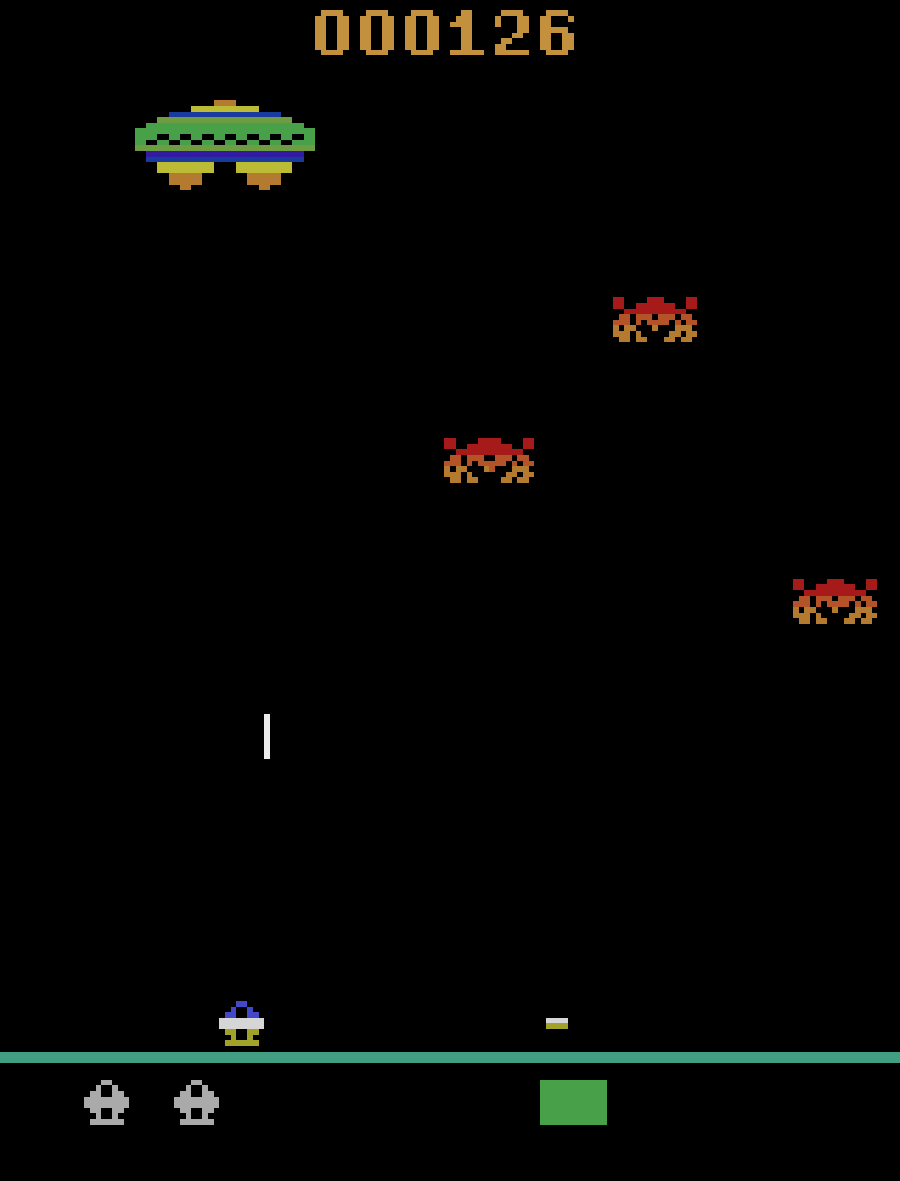
\includegraphics[width=\linewidth]{img/assault_preview.png}
    \caption{Atari Assault env.}
    \label{fig:assault_preview}
  \end{minipage}
\end{wrapfigure}

\textbf{Environment II: Atari Assault.} We consider the Atari game called Assault, where the agent controls a missile launcher to shoot oncoming alien ships while avoiding enemy missiles. The standard approach is to view this as a single-objective environment, where the agent's policy observes the entire image or the 128 byte raw RAM state observations to determine the optimal actions \citep{bellemare13arcade}. 
% This approach lacks transparency and interpretability, because the user will not know why the agent behaved in a certain way. \GS{This is not a good claim.}

For our modular framework, we break the objective down to a multi-objective problem, where each alien ship is viewed as a separate objective, and each local policy attempts to destroy its assigned target while avoiding enemy missiles. 
Not only does this facilitate an improvement in the performance, as we will demonstrate, but also we obtain a transparent design, because which target is being chased is revealed at each point. 
This modular design is made possible by the object-centric variant of the Atari environment \citep{delfosse2023ocatari}, which exposes the states of each individual target and the missiles by decoding the RAM states. 
The full observation space of each local policy also include the current position of the missile launcher, the current health, and the number of remaining lives. 
The local policy gets a reward or a penalty upon destroying its target enemy ship or losing a life, respectively. 
Lastly, we use the game score as the metric for evaluation.


\textbf{Baseline approaches.}
We compare our method against two baselines: a single policy PPO with weighted rewards and deep W-learning (DWN; \citet{rosero2024multi}). 
For the PPO baseline, since all the objectives have the same importance across the two environments, we use the total reward across objectives at each step as the reward function.
We note that in the Atari Assault environment we do not use the game score as a reward and instead use the same rewards perceived by the bidding-based policies to ensure a fair comparison.
The observation space remains the same as the multi-policy setting. 
In the Cat Feeder environment, we implement three reward mechanisms to help guide learning: one only with the sparse rewards from the environment, one with distance-based dense reward with respect to the nearest feeding request (denoted Nearest Shaping/NS in the experiments), and finally one where we provide distance-based reward with respect to the request that has the least amount of time until expiration (denoted Expiry Shaping/ES).
The PPO implementation is taken from CleanRL~\citep{huang2022cleanrl}.
We use the specified PPO hyperparameters from CleanRL for Atari Assault and we tune the hyperparameters for the Cat Feeder environment with 40 Optuna iterations~\citep{akiba2019optuna}.

DWN is another multi-policy method for multi-objective RL that uses DQN for each of the local policies and additionally learns a W-network for each policy that predict scalar weights. 
These weights are used to choose which policy's action should be played at each step. 
The W-network is trained alongside the Q-network by updating it with a gradient step to predict the negative temporal difference (TD) error when the policy does not get to play its action.
The assertion here is that the negative TD-error quantifies how important it is for the policy to play its action. 
The implementation is borrowed from the repository of \citet{rosero2024multi}. All hyperparameters for the baselines are listed in~\Cref{sec:reprod-details}.
\section{Experimental Results}\label{sec:experimental-results}

We evaluate the PPO implementation of our auction framework on evolving reachability objectives and a heterogeneous extension combining feeding priorities and battery charging.
We compare against centralized PPO and DWN, and ablate observations, pooling, and auction hyperparameters.
A detailed description of the environments and the baseline approaches is provided in Appendix~\ref{app:experimental setup}, below we include a summary.
The supplementary material includes our codebase and recorded rollouts of our bidding-based policies on the three base environments.

\textbf{Environments.}
We evaluate our approach on three environments: a mobile cat feeder environment, introduced in Section~\ref{sec:introduction}, and the two Atari games Assault and Air-raid.
In all these environments, the metric being optimized is the cumulative reward across all objectives.

In the Cat Feeder environment, a robot moves on a $30\times 30$ grid to feed up to $m$ cats that move stochastically.
Each cat disappears after a fixed number of steps; feeding it yields a reward, while disappearance incurs a penalty of equal magnitude.
We train with $m=8$ cats in the environment and demonstrate generalization up to $14$.
Each cat is served by a dedicated policy whose observation includes the robot position, the locations of active cats, and their remaining lifetimes.
We ablate global observations with attention pooling, global observations with fixed concatenation (no pooling), and local observations only (blind).

In both the Atari games---Assault (Figure~\ref{fig:assault_preview}) and Air-raid---the agent controls a missile launcher to destroy incoming alien ships while avoiding enemy missiles~\citep{bellemare13arcade}.
Although this is not traditionally seen as a multi-objective environment, we treat each ship as a separate objective and assign a local policy to pursue it, enabling a modular and interpretable design.
In lieu of the standard pixel observations, we employ the object-centric variant of the Atari environments~\citep{delfosse2023ocatari} which provides the environment state information to the policies.
Destroying a target yields reward, losing a life incurs a penalty.
We do not use attention pooling in the Atari games since there are only up to 3 targets.


\textbf{Baseline approaches.}
We compare against two baselines: a single PPO policy optimizing the objective-aggregated reward and deep W-learning (DWN)~\citep{rosero2024multi}.
These baselines also access the same object-centric observations in the Atari games.
The PPO baseline is implemented using CleanRL~\citep{huang2022cleanrl}.
Since we provide distance-based reward shaping to help our policies learn, to ensure a fair comparison, we test nearest-target and earliest-expiry distance shaping, as well as urgency-weighted scalarization of objective rewards, in Cat Feeder.
Hyperparameters are provided in~\Cref{sec:reprod-details}.
PPO parameters for Cat Feeder were tuned using 40 Optuna iterations~\citep{akiba2019optuna} while standard CleanRL Atari hyperparameters were used for the Atari games.
The centralized PPO baseline is trained with the same number of environment samples as our method.
DWN trains one DQN policy per objective together with W-networks that estimate urgency scores of states.
We use the same action window \(\tau\) for DWN.
Training budgets are fixed in advance: 400 PPO iterations for Cat Feeder and Air-Raid, and 150 for Assault.
For each of ten runs, one seed initializes the environment and algorithm; evaluation uses subsequent non-overlapping draws from that seeded stream, rather than independently chosen seed identifiers.


\begin{figure}%[h]
    \centering
    \begin{subfigure}{0.32\textwidth}
        \centering
        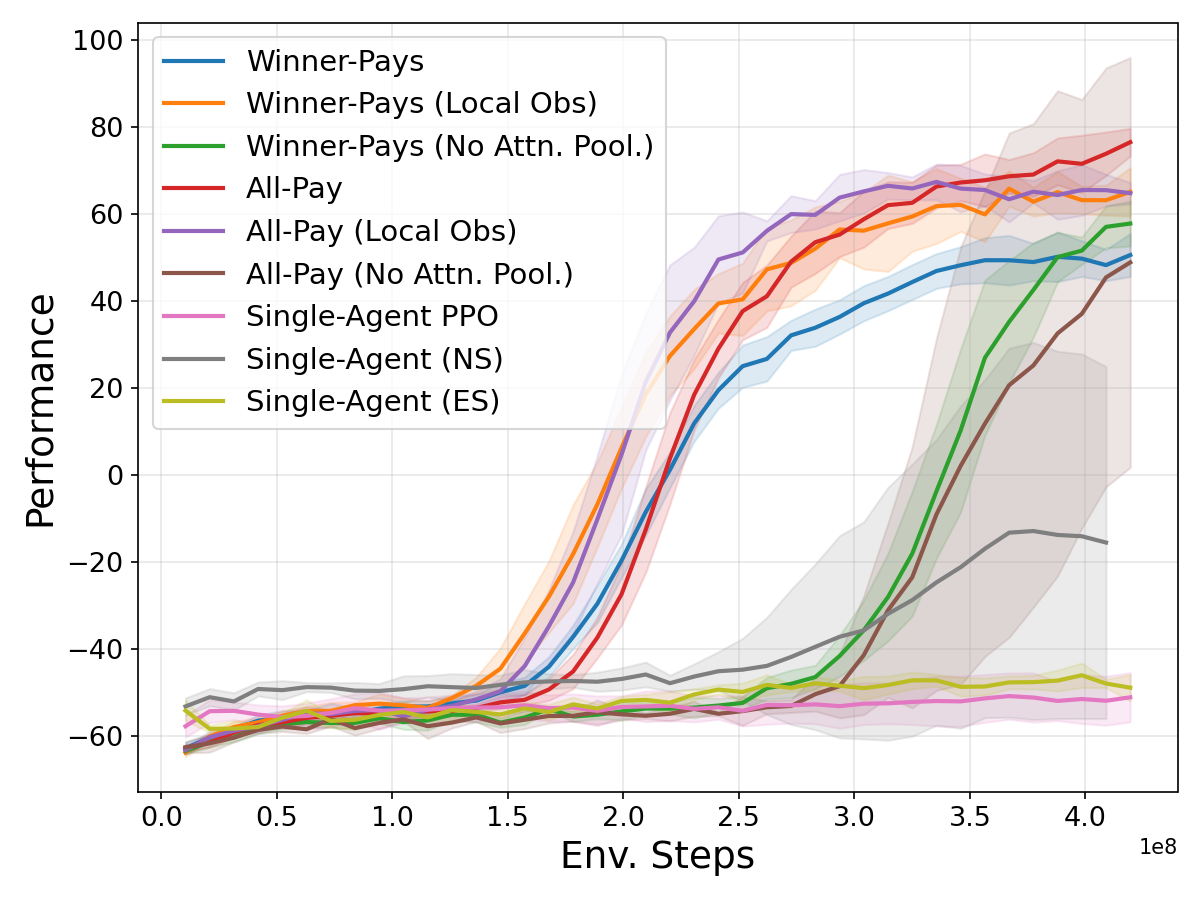
\includegraphics[width=\textwidth]{img/gridworld_bidding_mechanisms_learning_curves.png}
        % \caption{Cat Feeder: Learning curves}
        % \label{fig:dyntar-learning-curves}
    \end{subfigure}
    \hfill
    \begin{subfigure}{0.32\textwidth}
        \centering
        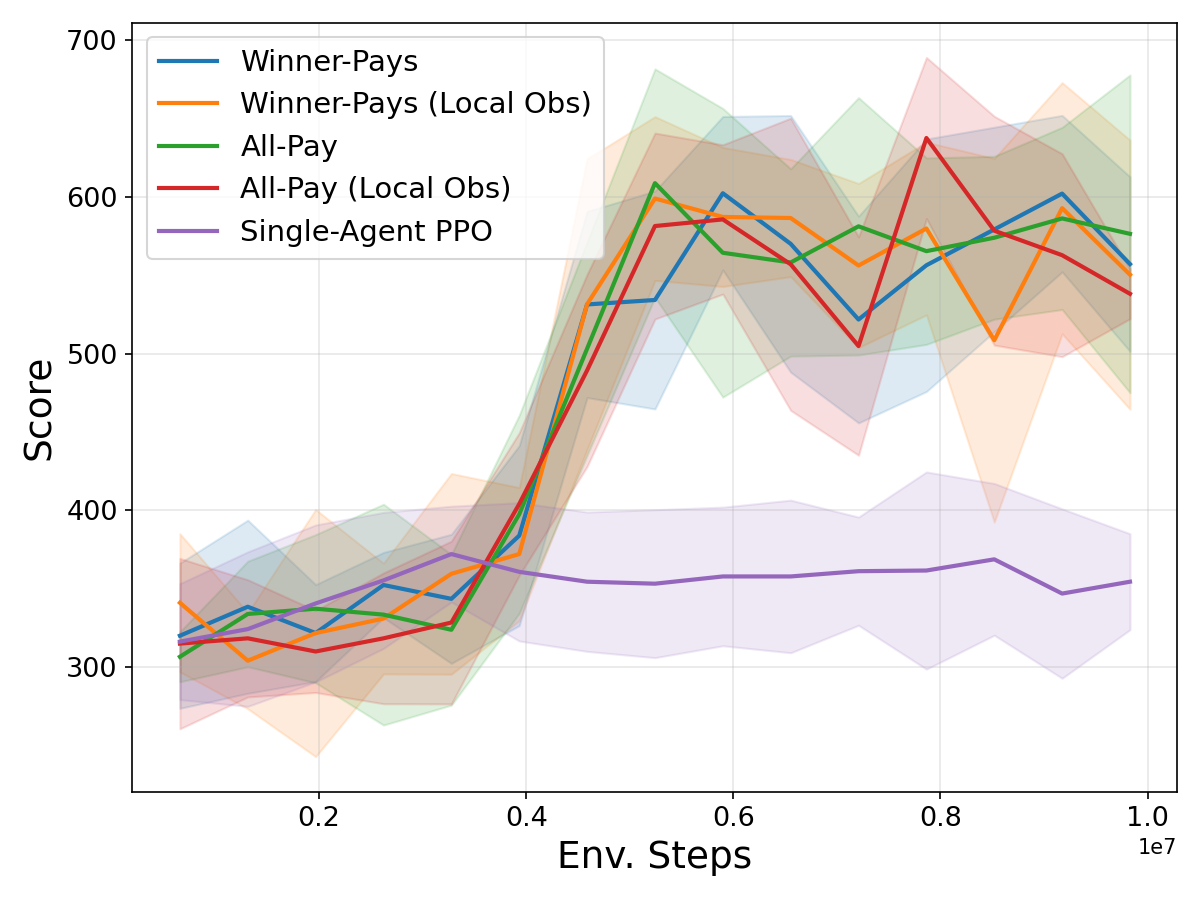
\includegraphics[width=\textwidth]{img/assault_bidding_mechanisms_learning_curves.png}
        % \caption{Atari Assault: Learning curves}
        % \label{fig:assault-learning-curves}
    \end{subfigure}
    \hfill
    \begin{subfigure}{0.32\textwidth}
        \centering
        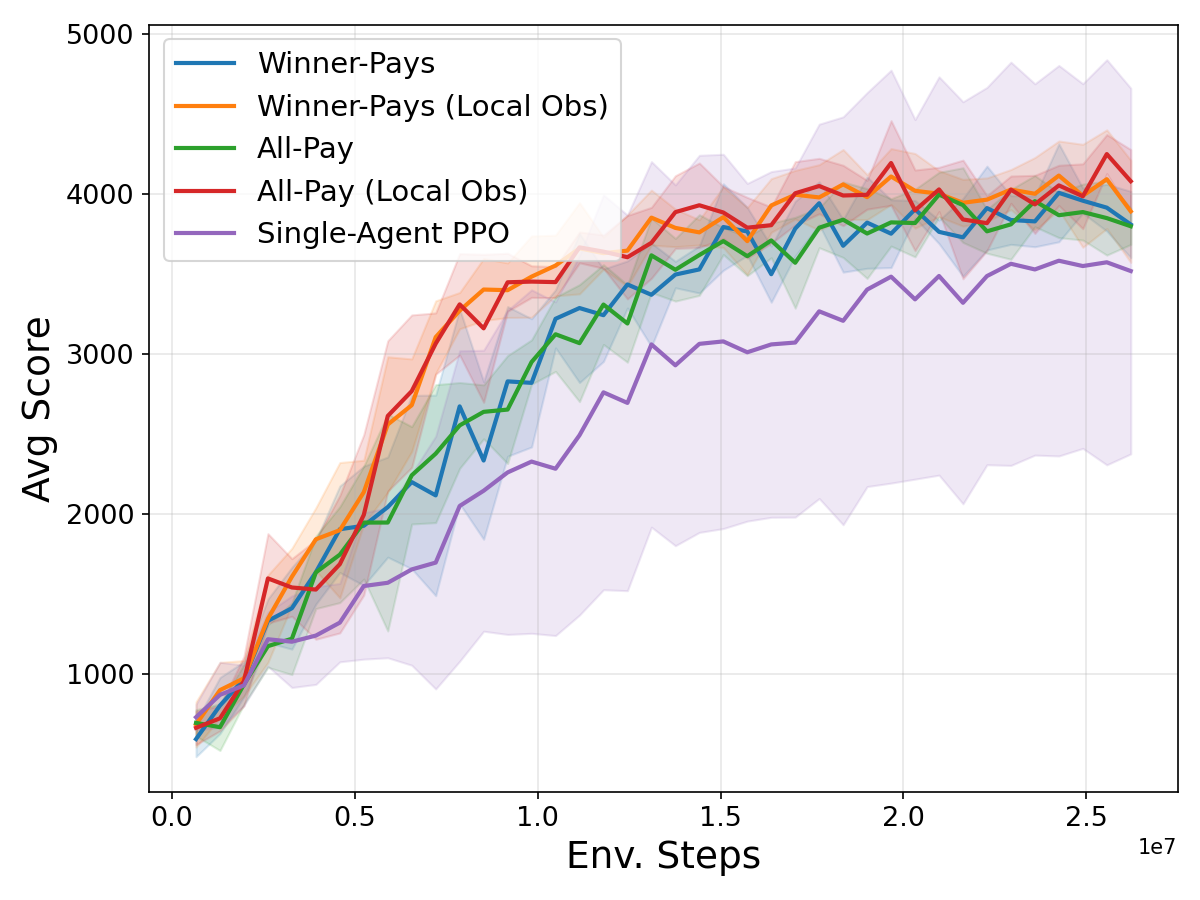
\includegraphics[width=\textwidth]{img/airraid_ppo_bidding_learning_curves_avg_score.png}
        % \caption{Atari Air-Raid: Learning curves}
        % \label{fig:airraid-learning-curves}
    \end{subfigure}
    \caption{Learning curves for different methods on Cat Feeder (left), Atari Assault (center), and Atari Air-Raid (right). We plot mean over 10 seeds at each evaluation iteration and the shaded region is \(\pm\) standard deviation across seeds.}
    \label{fig:learning-curves}
\end{figure}

% \begin{table}
  \centering
  \caption{Gridworld performance (mean $\pm$ std across available seeds) averaged over each seed's last 5 available evaluation iterations. Values are $8 \times \text{avg performance}$ for bidding/single-agent methods, and $8 \times \text{targets reached} - \text{expired}$ for DWN.}
  \begin{tabular}{ll}
    \hline
    {\bf Algorithm} & {\bf Performance} \\
    \hline
    Winner-Pays & $49.44$ {\small\textcolor{gray}{$(\pm 4.19)$}} \\
    Winner-Pays (Local Obs) & $63.76$ {\small\textcolor{gray}{$(\pm 3.85)$}} \\
    Winner-Pays (No Attn. Pool.) & $51.72$ {\small\textcolor{gray}{$(\pm 3.97)$}} \\
    All-Pay & $72.52$ {\small\textcolor{gray}{$(\pm 4.23)$}} \\
    All-Pay (Local Obs) & $64.96$ {\small\textcolor{gray}{$(\pm 3.82)$}} \\
    All-Pay (No Attn. Pool.) & $37.72$ {\small\textcolor{gray}{$(\pm 50.32)$}} \\
    DWN & $-10.27$ {\small\textcolor{gray}{$(\pm 2.38)$}} \\
    Single-Agent PPO & $-51.59$ {\small\textcolor{gray}{$(\pm 5.33)$}} \\
    Single-Agent (NS) & $-14.15$ {\small\textcolor{gray}{$(\pm 41.88)$}} \\
    Single-Agent (ES) & $-47.62$ {\small\textcolor{gray}{$(\pm 1.52)$}} \\
    \hline
  \end{tabular}
  \label{tab:gridworld_methods}
\end{table}

% \begin{table}
  \centering
  \caption{Assault score (mean $\pm$ std across available seeds) averaged over each seed's last 5 evaluation iterations.}
  \begin{tabular}{ll}
    \hline
    {\bf Algorithm} & {\bf Score} \\
    \hline
    Winner-Pays & $556.05$ {\small\textcolor{gray}{$(\pm 29.23)$}} \\
    Winner-Pays (Local Obs) & $557.55$ {\small\textcolor{gray}{$(\pm 36.92)$}} \\
    All-Pay & $576.64$ {\small\textcolor{gray}{$(\pm 43.19)$}} \\
    All-Pay (Local Obs) & $564.36$ {\small\textcolor{gray}{$(\pm 20.68)$}} \\
    DWN & $310.80$ {\small\textcolor{gray}{$(\pm 159.54)$}} \\
    Single-Agent PPO & $358.60$ {\small\textcolor{gray}{$(\pm 25.99)$}} \\
    \hline
  \end{tabular}
  \label{tab:assault_methods}
\end{table}

\begin{table}
  \caption{Scores: mean (standard deviation) across 10 seeds. For all PPO variants, including local observations only, each seed average uses its last 5 available evaluation checkpoints (evaluations every 10 PPO iterations, 20 rollouts each). Cat Feeder score is completed minus expired requests; Atari scores are game scores.}
  \label{tab:all_methods_comp}
  \centering
  \begin{tabular}{llll}
    \toprule
    {\bf Method} & {\bf Cat Feeder} & {\bf Atari Assault} & {\bf Atari Air-raid} \\
    \midrule
    Winner-Pays & $49.44$ {\small\textcolor{gray}{$(4.19)$}} & $556.05$ {\small\textcolor{gray}{$(29.23)$}} & $\textbf{3902.55}$ {\small\textcolor{gray}{$(90.44)$}} \\
    \textcolor{gray}{\itshape\hspace{1em}w. No Attn. Pool.} & \textcolor{gray}{\itshape $51.72$ {\small$(3.97)$}} & \textcolor{gray}{\itshape ---} & \textcolor{gray}{\itshape ---} \\
    \textcolor{gray}{\itshape\hspace{1em}w. Local Obs. Only} & $55.80$ {\small\textcolor{gray}{$(11.42)$}} & --- & --- \\
    All-Pay & $\textbf{72.52}$ {\small\textcolor{gray}{$(4.23)$}} & $\textbf{576.64}$ {\small\textcolor{gray}{$(43.19)$}} & $\textbf{3870.45}$ {\small\textcolor{gray}{$(76.72)$}} \\
    \textcolor{gray}{\itshape\hspace{1em}w. No Attn. Pool.} & \textcolor{gray}{\itshape $37.72$ {\small$(50.32)$}} & \textcolor{gray}{\itshape ---} & \textcolor{gray}{\itshape ---} \\
    \textcolor{gray}{\itshape\hspace{1em}w. Local Obs. Only} & $67.55$ {\small\textcolor{gray}{$(3.79)$}} & --- & --- \\
    \midrule
    DWN & $-10.27$ {\small\textcolor{gray}{$(2.38)$}} & $310.80$ {\small\textcolor{gray}{$(159.54)$}} & $2438.38$ {\small\textcolor{gray}{$(625.97)$}} \\
    Single-Policy PPO & \textcolor{gray}{\itshape ---} & $\textbf{358.60}$ {\small\textcolor{gray}{$(25.99)$}} & $\textbf{3549.33}$ {\small\textcolor{gray}{$(1170.14)$}} \\
    \textcolor{gray}{\itshape\hspace{1em}w. No Reward Shaping} & \textcolor{gray}{\itshape $-51.59$ {\small$(5.33)$}} & \textcolor{gray}{\itshape ---} & \textcolor{gray}{\itshape ---} \\
    \textcolor{gray}{\itshape\hspace{1em}w. Nearest Shaping} & \textcolor{gray}{\itshape $-14.15$ {\small$(41.88)$}} & \textcolor{gray}{\itshape ---} & \textcolor{gray}{\itshape ---} \\
    \textcolor{gray}{\itshape\hspace{1em}w. Expiry Shaping} & \textcolor{gray}{\itshape $-47.62$ {\small$(1.52)$}} & \textcolor{gray}{\itshape ---} & \textcolor{gray}{\itshape ---} \\
    \textcolor{gray}{\itshape\hspace{1em}w. Urgency Weighting} & $51.78$ {\small\textcolor{gray}{$(14.31)$}} & --- & --- \\
    \bottomrule
  \end{tabular}
\end{table}



\textbf{Learning dynamics.}\quad \Cref{fig:learning-curves} shows the learning curves for multi-policy bidding and single-policy PPO algorithms on the three environments.
While the curves are more noisy with Atari Assault, they exhibit clearly distinguishable sigmoidal shapes with the other two environments.
The curves for \allpay and \poorman methods start growing around the same time.
\textbf{The variants without attention pooling for targets only start learning much later.}
This validates the use of the attention pooling architecture to learn useful embeddings of targets.
We remark that, based on the multi-agent PPO recipe of Yu et al.~\citep{yu2022mappo}, we also found that using a small clip coefficient (\({\sim}0.05\)) and large batch sizes was crucial to obtain stable but slower convergence of the policies towards an equilibrium.

\textbf{Comparison with baselines.}\quad \Cref{tab:all_methods_comp} lists performance across the three base environments.
Urgency-weighted scalarization raises centralized PPO's Cat Feeder score to $51.78\pm14.31$, comparable in mean to Winner-Pays ($49.44\pm4.19$), while All-Pay achieves $72.52\pm4.23$.
Thus the stronger baseline changes the comparison materially: All-Pay retains an advantage, whereas Winner-Pays does not outperform urgency-weighted PPO in mean score.
Separating objective rewards may ease credit assignment, but these comparisons do not isolate its causal contribution.
In Assault, single extracted frames may omit velocities and projectile directions; the four-frame observations in Air-Raid may reduce this partial observability.
We did not conduct a dedicated frame-stack ablation, so this remains a possible explanation rather than an established effect.

DWN is included as a closely related multi-policy MORL method that learns a state-dependent arbitration signal.
Its low scores suggest that TD-error-based arbitration is less effective in these experiments; they do not establish that its architecture alone causes the difference.
Our empirical comparisons concern this PPO implementation, rather than a general replacement for PPO across domains.

\textbf{Observations and pooling.}\quad
The non-pooled variants retain all target information through fixed concatenation.
Winner-Pays scores with and without pooling ($49.44\pm4.19$ versus $51.72\pm3.97$) are close relative to the across-seed variation; this does not establish superiority of the non-pooled architecture.
Pooling supports variable-size objective sets and earlier learning in the reported curves.
All-Pay with pooling has a higher mean than its blind variant ($67.55\pm3.79$); blind Winner-Pays has a higher mean ($55.80$) but greater variability ($11.42$), so the observations do not show a consistent final-score benefit for both auction mechanisms.

\textbf{Heterogeneous objectives and priorities.}\quad
We extend Cat Feeder to eight cats with feeding priorities from 1 to 4 and three charging stations, all moving stochastically on a $30\times30$ grid.
The robot has a capacity-50 battery; depletion away from a station triggers a tow and refill.
One local policy serves each cat, and a separate charging policy receives a battery-dependent effective bid boost (Appendix~\ref{app:heterogeneous-implementation}).
Feeding rewards scale with cat priority.
Table~\ref{tab:heterogeneous-cat-feeder} reports the sum of priorities of fed cats and battery depletions, against centralized PPO with an unweighted reward sum.
All-Pay achieves a higher feeding score and fewer battery depletions than centralized PPO, demonstrating coordination across feeding and charging objectives; the nonzero depletion rate does not constitute a safety guarantee.
Appendix~\ref{app:heterogeneous-results} reports feeding counts by priority.

\begin{table}[t]
  \caption{Heterogeneous Cat Feeder: mean (standard deviation) of priority-weighted feeding score and battery depletions. Higher feeding scores and fewer depletions are better.}
  \label{tab:heterogeneous-cat-feeder}
  \centering
  \begin{tabular}{lrr}
    \toprule
    Method & Feeding priority sum & Battery depletions \\
    \midrule
    All-Pay & $194.56\;(4.67)$ & $0.07\;(0.05)$ \\
    Centralized PPO & $111.86\;(57.08)$ & $3.81\;(5.03)$ \\
    \bottomrule
  \end{tabular}
\end{table}


\begin{figure}[h]
    \centering
    \begin{subfigure}[t]{0.31\textwidth}
        \centering
        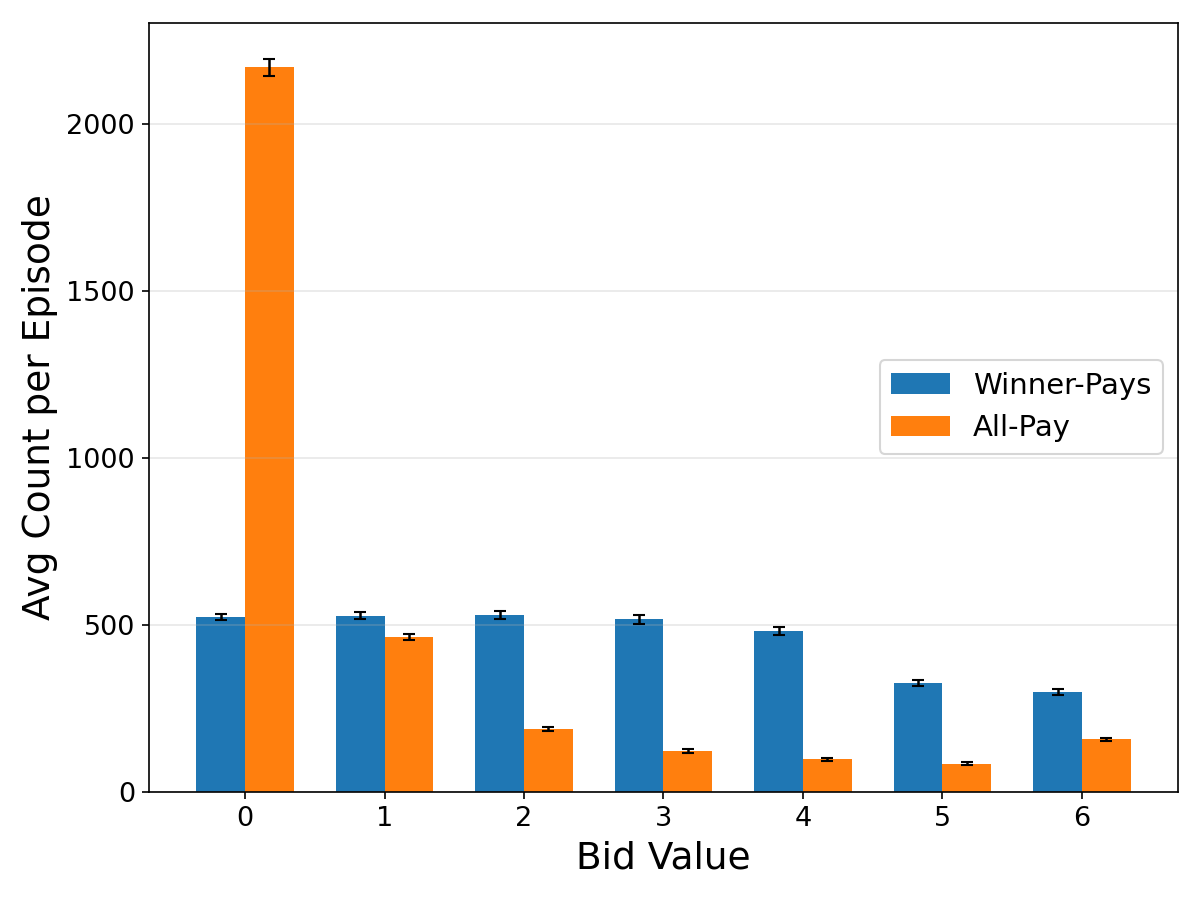
\includegraphics[width=\textwidth]{img/bidding_mechanisms_bid_distribution.png}
        \caption{Cat Feeder: Bid distribution}
        \label{fig:dyntar-bid-dist}
    \end{subfigure}
    \hfill
    \begin{subfigure}[t]{0.25\textwidth}
        \centering
        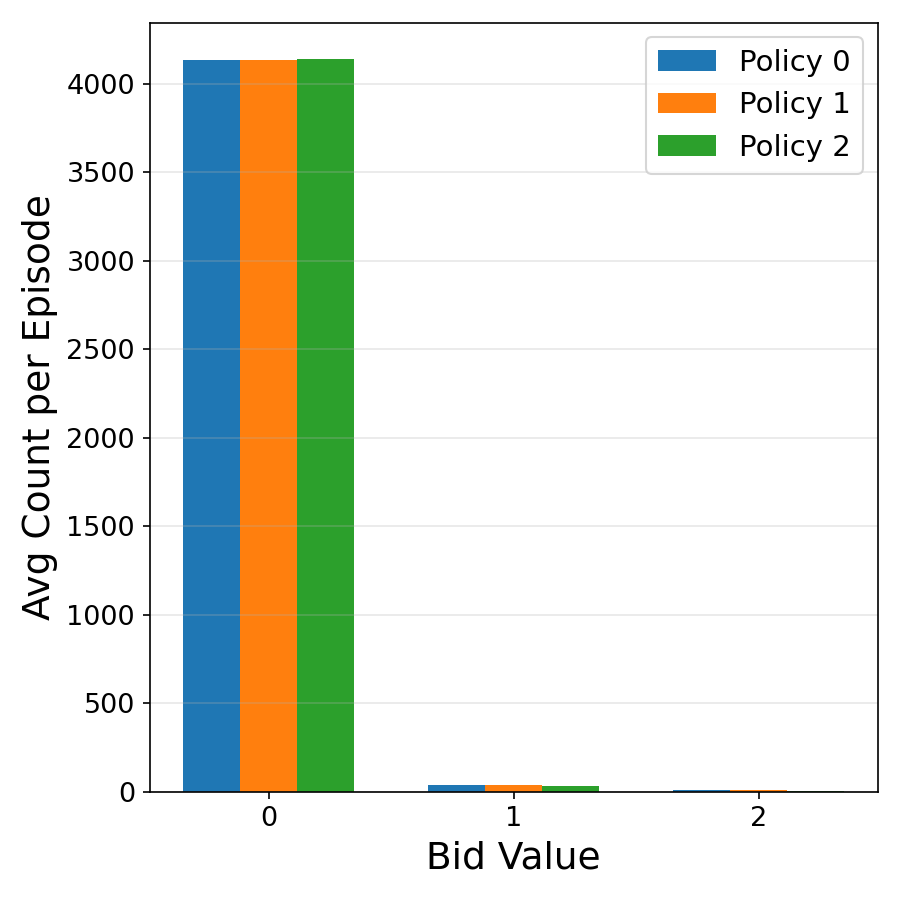
\includegraphics[width=\textwidth]{img/assault_bid_distribution_winner-pays.png}
        \caption{Atari Assault: Bid distribution (\poorman)}
        \label{fig:assault-bid-dist}
    \end{subfigure}
    \hfill
    \begin{subfigure}[t]{0.25\textwidth}
        \centering
        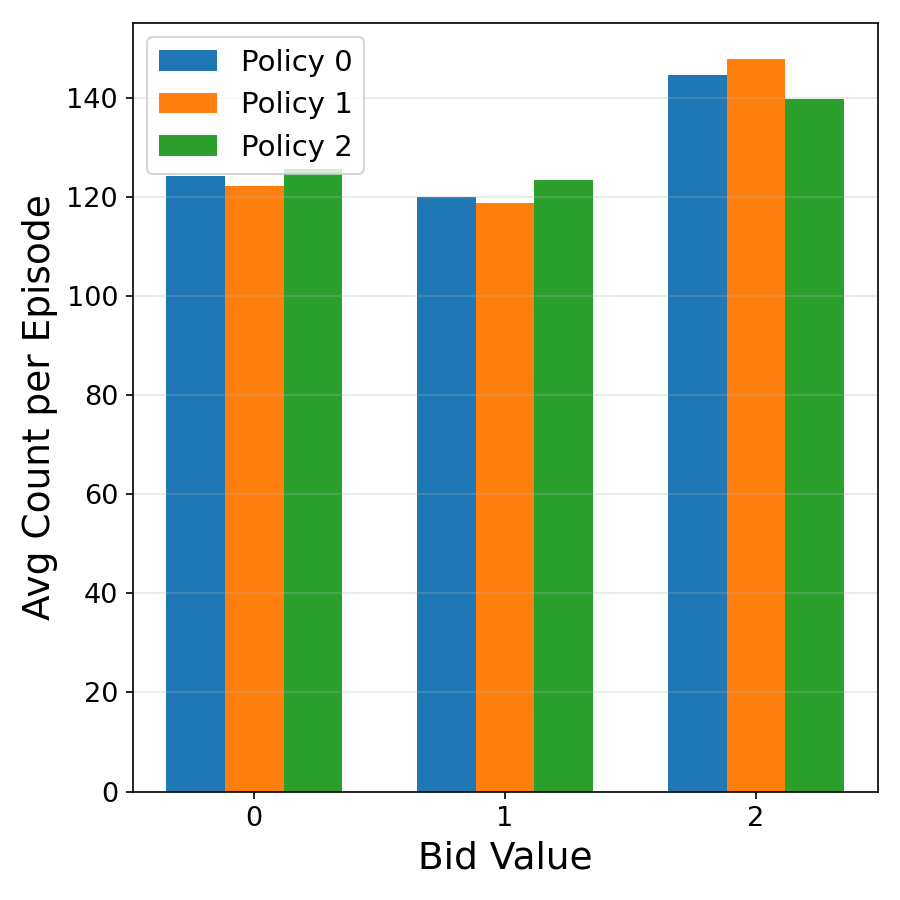
\includegraphics[width=\textwidth]{img/airraid_bid_distribution_winner_pays.png}
        \caption{Atari Air-Raid: Bid distribution (\poorman)}
        \label{fig:airraid-bid-dist}
    \end{subfigure}
    \caption{Comparison of bid distributions across environments and methods. Bars show aggregate bid counts for each bid value across all policies.}
    \label{fig:control-bid-dist}
\end{figure}

\begin{figure}
    \centering
    \begin{subfigure}[b]{0.3\textwidth}
        \centering
        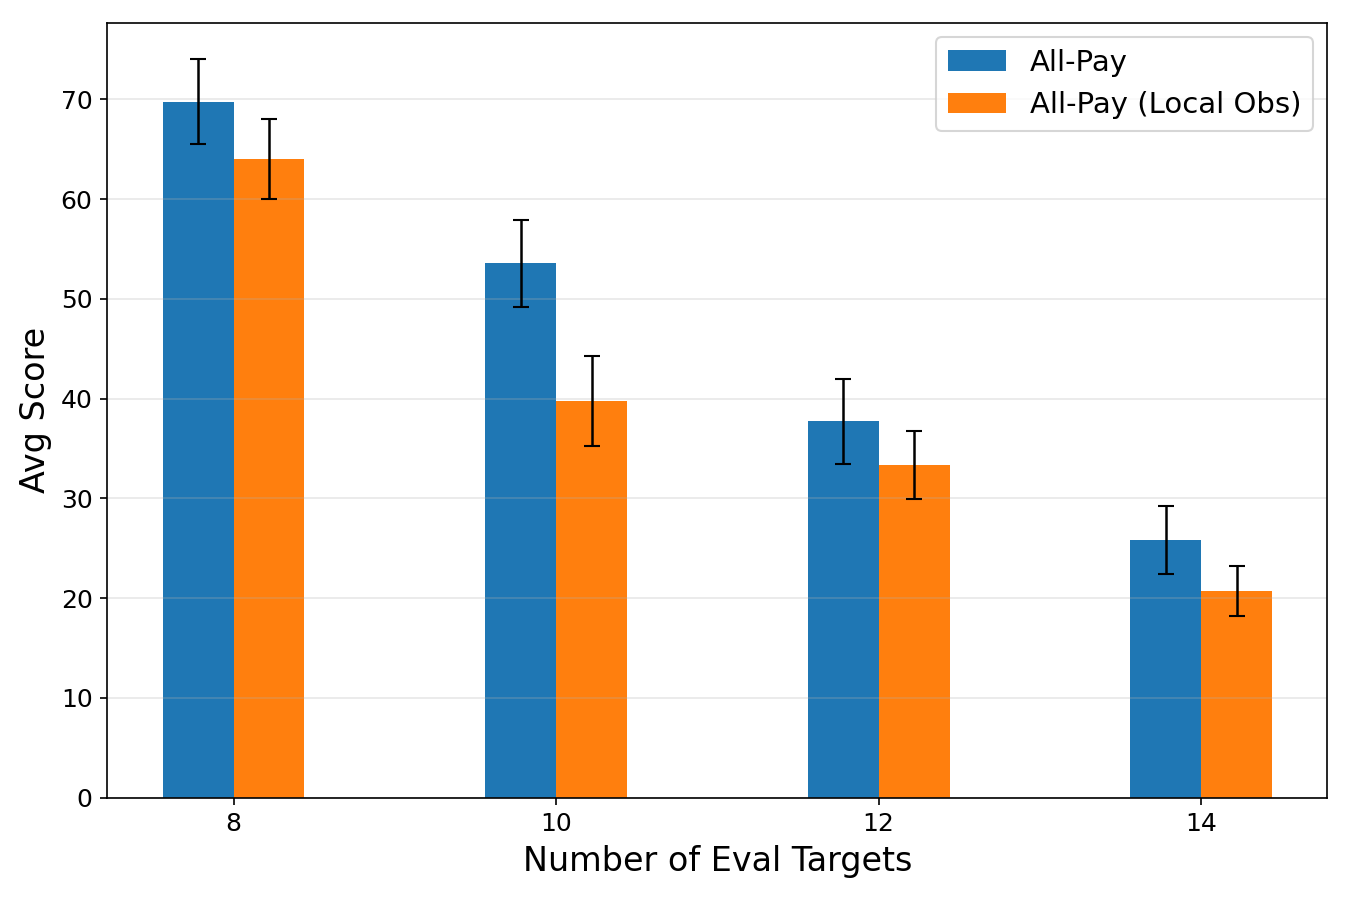
\includegraphics[width=\textwidth]{img/bidding_mechanism_scaling.png}
        \caption{Scaling number of targets.}
        \label{fig:bidding-mechanism-scaling}
    \end{subfigure}
    \hfill
    \begin{subfigure}[b]{0.3\textwidth}
        \centering
        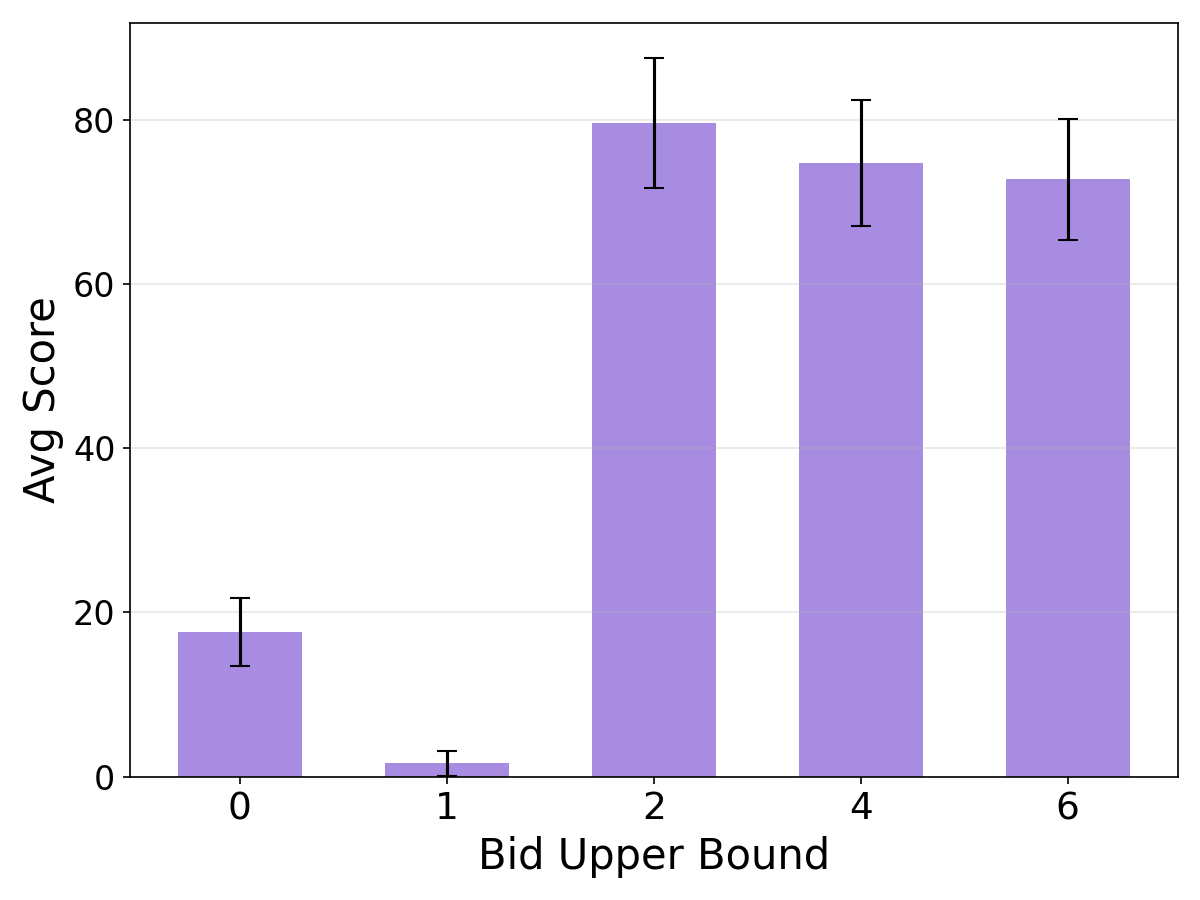
\includegraphics[width=\textwidth]{img/gridworld_bid_upper_bound_bar_chart.png}
        \caption{Ablation: Bid upper bound}
        \label{fig:gridworld-bid-upper-bound}
    \end{subfigure}
    \hfill
    \begin{subfigure}[b]{0.3\textwidth}
        \centering
        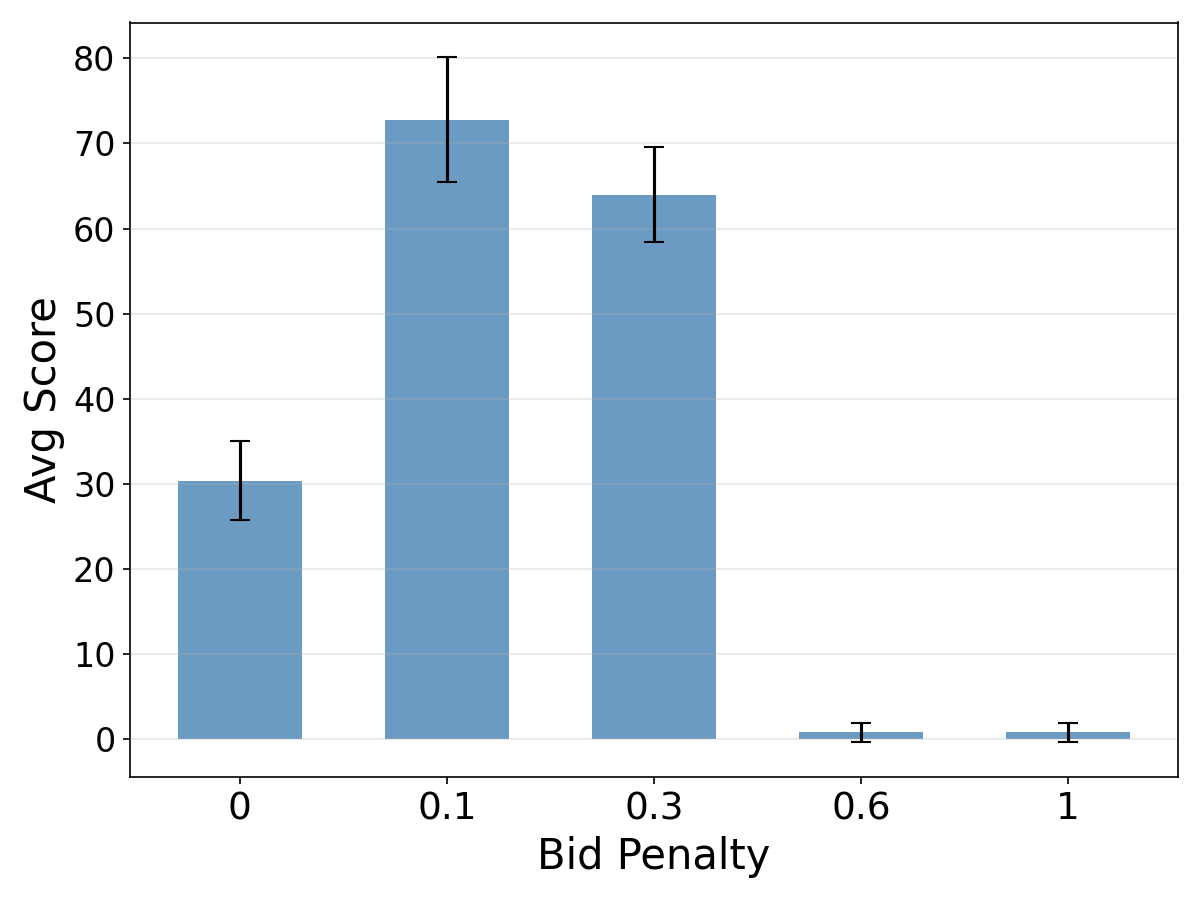
\includegraphics[width=\textwidth]{img/gridworld_bid_penalty_bar_chart.png}
        \caption{Ablation: Bid penalty}
        \label{fig:gridworld-bid-penalty}
    \end{subfigure}
    \caption{Scaling number of targets and ablations on the Cat Feeder environment.}
    \label{fig:ablations}
\end{figure}



\textbf{Policy behaviors and interpretability.}\quad
Video rollouts illustrate control allocation as each policy pursues its assigned objective; completion need not occur within one action window. \Cref{fig:control-bid-dist} presents the bid distributions.
% and control distributions are reported in Appendix~\ref{app:additional-experimental-results}.
In Assault, bids are usually 0, making allocation close to random tie-breaking; the gains here may arise primarily from objective decomposition rather than learned urgency arbitration. In contrast, the Cat Feeder environment shows a wider bid spread (0--6). Here, \allpay yields more conservative policies with mostly low bids, while \poorman produces a more even distribution, reflecting greater willingness to bid high.
Finally, in Air-raid, we see policies bidding the highest value more often, although they also bid lower values.
This is because there is a constant stream of enemy ships that each policy has to destroy and so they want to take control more often to avoid missing out on points.

\textbf{Scaling number of targets.}\quad We conduct an experiment with the Cat Feeder environment in which the number of cats seen during testing is larger than that during training.
This is achieved by deploying more copies of the same policy that optimize the additional objectives.
\Cref{fig:bidding-mechanism-scaling} evaluates transfer from eight training targets to as many as fourteen testing targets without retraining.
The plot uses eight times mean per-episode average performance; scaling selects a single best periodic checkpoint rather than averaging the final five.
With fixed episode length, more requests can expire as target count grows (Appendix~\ref{app:scaling-coverage}).
The minimum reported per-target completion count remains positive at every tested size (Appendix~\ref{app:scaling-coverage}), supporting continued service across all targets rather than constant performance as their number grows.

\textbf{Hyperparameter ablations.}\quad \Cref{fig:gridworld-bid-upper-bound} shows that at least two bid levels are needed for good performance; with only one level, policies cannot compete effectively. \Cref{fig:gridworld-bid-penalty} evaluates the bid penalty factor: without penalties all policies overbid, hurting performance, while overly large penalties discourage bidding. Additional action-window ablations are reported in Appendix~\ref{app:additional-experimental-results}.

\section{Limitations}
While our auction-based multi-policy mechanism can produce strong performance in a vast range of challenging environments, there are also instances where our mechanism produces suboptimal results. 
For instance, consider a setup where the cat feeder robot has to choose between going left or right.
On the left there are two cats and on the right there is only one cat, but the robot only has time to pick one direction.
The optimal action to maximize cumulative reward is to go left.
However, if all the local policies bid the highest value possible, due to random tie-breaking, our mechanism would instruct the robot to go left with probability $2/3$.
This motivates future study that attempts using different mechanisms like majority voting---which would result in the optimal action in the example above.

\section{Conclusion and Future Directions}
We consider the problem of adapting RL policies due to evolving objectives, where any number of objectives may appear or disappear at runtime, and the agent must adapt as swiftly as possible.
We present a compositional solution where each objective is served using a dedicated local policy, and each local policy competes against the other policies through an auction-based mechanism to select its preferred action.
The training is formulated as a nonzerosum game between the local policies, and it is implemented using PPO in our framework.
Using two challenging benchmarks, we demonstrate that our framework produces interpretable policies that achieve superior learning rate and  dramatic performance improvement compared to the baseline approaches.

While we have only considered multi-objective environments in which the objectives belong to the same family, we will extend the framework to combinations of objective classes. 
The difficulty lies in the fact that a policy learned to compete against opponents from a given class may not work against opponents for a novel class of objectives seen at runtime.
Additionally, richer bidding mechanisms might be necessary. 
For instance, while combining reachability and safety objectives, usually safety needs to get the priority when there is a tie in the bidding, instead of a random resolution.


\FloatBarrier
\clearpage
\begin{ack}
Guruprerana Shabadi is supported by NSF Award SLES 2331783.
Kaushik Mallik is supported by the grant RYC2024-049116-I funded by MICIU/AEI/10.13039/501100011033 and the ESF+.
\end{ack}

\bibliographystyle{plainnat}
\bibliography{main}


%%%%%%%%%%%%%%%%%%%%%%%%%%%%%%%%%%%%%%%%%%%%%%%%%%%%%%%%%%%%

\clearpage
\appendix

\section{A Deterministic Time-Bounded Path Planning Problem}

%\smallskip\noindent
%\textbf{Lower complexity bound.}\todo{this part needs work}
%We establish that the optimal policy synthesis problem is NP-hard, and we show this already on a simplified setting:
%	Suppose the transition function $T$ of the \momdp is deterministic, the goals are stationary such that the location of the $i$-th goal is always $g_i\in S$, and for any policy, the minimum travel time from a given location $x\in S$ to the $i$-th goal is $t_i = d(x,g_i)$. 
%	(Alternatively, $t_i$ can be interpreted as the length of the shortest path from $x$ to $g_i$ when the agent moves at the unit velocity.)
%
%\begin{theorem}\label{thm:np hardness}
%	Finding the optimal policy for the \momdp is NP-hard.
%\end{theorem}
%
%\begin{proof}
%	The simpler setting with deterministic agents and stationary goals subsumes the Euclidean traveling salesman problem, where the deadlines are all infinity, and the goal is to find the shortest path passing through all the goals.
%	This problem is known to be NP-complete~\cite{DBLP:journals/tcs/Papadimitriou77}, and our deadline-restricted case is at least as hard as it.
%	\KM{There is a slight difference, that we allow revisiting a state. However, I found on discussion forums that this does not change the complexity, find a reference. Also see metric traveling salesman, which is more general (we could then replace the Euclidean distance requirement in the \momdp state space with the requirement of just having a metric.}
%\end{proof}
%
%The NP-hardness of the optimal policy synthesis problem motivates us to find heuristics to solve the problem.
%Moreover, our heuristic must seamlessly support dynamic addition or deletion of objectives (modeled as reward functions), which is our ultimate goal.
%Towards our goal, we identify a key structural property of the optimal policy below.

We consider a path planning problem for an agent, where the agent needs to reach multiple stationary goals $\{g_i\}_{i=[1;m]}$ in the state space, each goal $g_i$ has a deadline $d_i\in \mathbb{N}_{>0}$ before which it must be reached, the agent receives a reward $r_i\in \mathbb{R}_{>0}$ if the goal $g_i$ is reached before $d_i$, and receives a penalty $-M$ otherwise.
Moreover, we assume that agent's movement has no uncertainties.
This problem can be modeled as an \momdp $\M_d$ where $S = L\times \mathbb{N}_{\geq 0}$ consists of the agent's locations $L$ and time $t$, 
actions consist of the agent's movement in $L$,
the transition kernel is a deterministic function that models the agent's change in position and the passage of time, 
the initial state is $(l,0)$ for some $l\in L$,
the reward functions are as described earlier, 
and the horizon $H$ is given.
Our objective is to compute the optimal policy 

\begin{proposition}\label{prop:scheduling is the optimal choice}
	Consider the simpler case of deterministic agent with stationary goals.
	There exists a permutation $\sigma^*\in \Sigma_m$, where $\Sigma_m$ is the set of all permutations of $[1;m]$, such that the optimal policy $\pi^*$ pursues the goals in the order $\sigma^*(1)\ldots\sigma^*(m)$, and $\pi^*$ takes the shortest paths from the initial agent location to goal $\sigma^*(1)$ and between $\sigma^*(i)$ and $\sigma^*(i+1)$, for every $i\in [1;m-1]$.
\end{proposition}
The above proposition effectively reduces the problem to an optimal \emph{scheduling} problem.
Furthermore, Theorem~\ref{thm:np hardness} suggests that a polynomial-time centralized optimal algorithm does not exist, unless P=NP, already for the simpler deterministic case with stationary goals.
This motivates us to seek for a heuristic approach that is aimed towards finding the optimal schedule over the goals whose existence is guaranteed by Proposition~\ref{prop:scheduling is the optimal choice}.

A natural deterministic baseline is the \emph{least slack time first} (LSTF) rule, which schedules the goal with smallest slack $\slack_i(x,t)\coloneqq d_i-t-d(x,g_i)$.
However, this notion of urgency is tailored to stationary goals and deterministic travel times, and does not align with our full \momdp objective once targets move stochastically or may appear and disappear over time.
For this reason, we use a more general benchmark that we call \emph{reward-aware urgency first} (RAUF).
\KM{Is this used in the literature? If yes, some citation would be nice.}
At every decision point, RAUF selects one of the goals with maximal \emph{reward-aware urgency}, namely the marginal continuation-value gain from granting that goal immediate control rather than deferring control to competing goals; ties are broken uniformly at random.
Unlike slack, this urgency notion directly accounts for discounted rewards, missed-deadline penalties, stochastic target motion, and future target arrivals or removals.
Our auction mechanism is designed to approximate this reward-aware urgency ordering in a decentralized manner while remaining tractable in settings where computing the globally optimal schedule is infeasible.
\GS{Also talk about how urgency encodes agent cooperation.}


\section{Proof of the \poorman Control-Gain Result}
\label{app:poorman-control-gain-proof}

\begin{proof}[Proof of Theorem~\ref{thm:poorman-favors-high-control-gain}]
	Suppose for contradiction, some other policy $j\neq i^*$ wins control by bidding $b_j$, while policy $i^*$ bids $b_{i^*}<b_j$. 
	As this is a Nash equilibrium, it must hold that 
	$U_{j,t}^{\mathsf{P}}(s,b_j) > \widetilde V^{\lose}_{j,t}(s)$, i.e., $G_{j,t}(s) - \rho b_j > 0$,
	because otherwise, policy $j$ would be better off by losing the bidding instead.
	This gives us the upper bound $\rho b_j < G_{j,t}(s)$.
	It follows from $\rho\beta > \max_{k\in [1;m]}G_{k,t}(s)$ that $\rho b_j < \rho\beta$, and hence $b_j<\beta$, i.e., the policy $j$ does not make the maximum bid.
	
	Now we assumed that policy $i^*$ had bid $b_{i^*}<b_j$, but we show that policy $i^*$ would achieve a higher one-round bidding payoff by bidding $b_j+1$ (valid, since $b_j<\beta\implies b_j+1\leq \beta$), contradicting the Nash equilibrium:	 
$	U_{i^*,t}^{\mathsf{P}}(s,b_j+1) 
	= \widetilde V^{\lose}_{i^*,t}(s)+G_{i^*,t}(s) - \rho(b_j+1) 
	= \widetilde V^{\lose}_{i^*,t}(s)+ G_{i^*,t}(s) - \rho b_j -\rho  
	> \widetilde V^{\lose}_{i^*,t}(s)+ G_{i^*,t}(s) - G_{j,t}(s) -\rho
	> \widetilde V^{\lose}_{i^*,t}(s) = U_{i^*,t}^{\mathsf{P}}(s,b_j)
$.
\end{proof}

\section{Proof of the \allpay Control-Gain Result}
\label{app:allpay-control-gain-proof}

\begin{proof}[Proof of Theorem~\ref{thm:allpay-favors-high-control-gain}]
	It follows from the work of Baye et al.~\cite{baye1996all} that in the Nash equilibrium, the optimal bid of the policies are as follows.
	The policy $i^*$ picks a uniformly random bid $b_i^*$ from $[0,G_{j^*,t}/\rho]$, the policy $j^*$ picks a uniformly random bid $b_j^*$ from $(0,G_{j^*,t}/\rho]$ while picking the bid $0$ with probability $(G_{i^*,t} - G_{j^*,t})/G_{i^*,t}$, and every other policy $k\notin\{i^*,j^*\}$ deterministically picks the bid $0$.
	Clearly, if $b_i^*>b_j^*$, then $i^*$ wins control, and we need to show that $P[b_i^* > b_j^*]  = 1- \sfrac{G_{j^*,t}}{2G_{i^*,t}}$.
	To show this, consider the probability density function $f_{i^*}(b) = \sfrac{\rho }{G_{j^*,t}}$ of $b_{i^*}$, and the cumulative distribution function $F_{j^*}(b) = (G_{i^*,t} - G_{j^*,t})/G_{i^*,t} + \sfrac{\rho b}{G_{i^*,t}}$ of $b_{j^*}$.
	Then,
	\begin{align*}
		P[b_i^* > b_j^*] 
		&= \int_{-\infty}^\infty F_{j^*}(b)f_{i^*}(b)db\\
		&= \int_{0}^{G_{j^*,t}/\rho} \left(\frac{G_{i^*,t} - G_{j^*,t}}{G_{i^*,t}} + \frac{\rho b}{G_{i^*,t}}\right)\cdot \frac{\rho }{G_{j^*,t}} \cdot db \\
		&= \int_{0}^{G_{j^*,t}/\rho} \frac{G_{i^*,t} - G_{j^*,t}}{G_{i^*,t}} \cdot \frac{\rho }{G_{j^*,t}} \cdot db
		+ \int_{0}^{G_{j^*,t}/\rho} \frac{\rho b}{G_{i^*,t}}\frac{\rho }{G_{j^*,t}} \cdot db\\
		&=  \frac{G_{i^*,t} - G_{j^*,t}}{G_{i^*,t}} \cdot \frac{\rho }{G_{j^*,t}} \cdot \frac{G_{j^*,t}}{\rho}
		+ \frac{\rho^2}{G_{i^*,t}G_{j^*,t}}\cdot \frac{\left(G_{j^*,t}\right)^2}{2\rho^2}\\
		&= \frac{G_{i^*,t} - G_{j^*,t}}{G_{i^*,t}} + \frac{G_{j^*,t}}{2G_{i^*,t}}\\
		&= 1-\frac{G_{j^*,t}}{G_{i^*,t}} + \frac{G_{j^*,t}}{2G_{i^*,t}}\\
		&= 1-\frac{G_{j^*,t}}{2G_{i^*,t}}.
	\end{align*}
\end{proof}

%\section{Special Case: Relation to Least Slack Time First}
\label{app:lstf-analysis}

We now connect the auction mechanism to least slack time first (LSTF) in the deterministic stationary-goal setting from Appendix~\ref{app:deterministic-path-planning}.
Recall that each goal \(g_i\) is stationary, the agent moves deterministically, and \(d(x,g_i)\) is the minimum travel time from location \(x\) to goal \(g_i\).
At location \(x\) and time \(t\), define the slack of goal \(i\) by
\[
  \slack_i(x,t)\coloneqq d_i-t-d(x,g_i).
\]
Once \(g_i\) is reached, it disappears from the map and we write \(\slack_i(x,t)=\bot\).
The least slack time first rule schedules a goal with minimum nonnegative slack~\citep{brown2020optimal}.
Formally, at location \(x\) and time \(t\), LSTF selects any goal
\[
  i_{\mathrm{LSTF}}\in
  \arg\min_{i:\slack_i(x,t)\geq 0}
  \slack_i(x,t),
\]
with ties broken arbitrarily.
Thus LSTF gives control to the goal whose deadline is closest after accounting for travel time.

We show that, when one goal is critically urgent and all other goals are safely non-urgent, the auction selects the same goal as LSTF.
At each bidding round, every goal \(i\) is represented by a local policy that proposes an action and submits a nonnegative bid.
The highest bidder controls the agent for the next \(\tau\in\mathbb{N}_{>0}\) time steps, with ties broken uniformly at random.
Bids are bounded by \(\beta\), and \(\rho>0\) is the bid penalty coefficient.
For \poorman, bids are integer values in \([0;\beta]\); for \allpay, bids are real values in \([0,\beta]\).
We analyze two payment rules: in \poorman, only the winning policy pays \(\rho b_i\), while in \allpay, every policy pays \(\rho b_i\).

In the remainder of this appendix, \(s\in L\) denotes the current agent location and \(t\) denotes the current time.
Suppose \(\pi_i\) is the local policy for the \(i\)-th goal, mapping each pair \((s,t)\) to a bid \(b_i\) and an action \(a_i\).
We write \(\pi_i^b\colon (s,t)\mapsto b_i\) and \(\pi_i^a\colon (s,t)\mapsto a_i\) for the bidding and action components.
In this deterministic setting, \(\pi_i^a\) proceeds toward its goal \(g_i\) along a shortest path, and \(T^\tau(s,\pi_i^a)\) denotes the state reached by applying \(\pi_i^a\) for \(\tau\) steps from \(s\).

For a bidding round at time \(t\), define \(V_i^{\win}(s,t,b_i)\) and \(V_i^{\lose}(s,t,b_i)\) as the value to policy \(i\) when it bids \(b_i\) and respectively wins or loses the next bidding interval.
Let \(V_i^{\cont}(s,t)\) denote the Nash equilibrium continuation value of the subgame starting from \((s,t)\).
The value functions are defined by backward induction as
\begin{align*}
  V_i^{\win}(s,t,b_i)
  &\coloneqq
  \gamma^\tau V_i^{\cont}(T^\tau(s,\pi_i^a),t+\tau)-\rho b_i,\\
  V_i^{\lose}(s,t,b_i)
  &\coloneqq
  \gamma^\tau V_i^{\cont}(T^\tau(s,\pi_j^a),t+\tau)-\rho b_i\cdot \mathbf{1}[\text{\allpay}],
\end{align*}
where \(j\) is the policy that wins control when \(i\) loses.
The net gain from winning rather than losing is
\begin{align*}
  \Delta_i^{\mathrm{net}}(s,t,b_i)
  &\coloneqq
  V_i^{\win}(s,t,b_i)-V_i^{\lose}(s,t,b_i)\\
  &=
  \Delta_i^{\mathrm{gross}}(s,t)-\rho b_i\cdot \mathbf{1}[\text{\poorman}],
\end{align*}
where the gross gain
\[
  \Delta_i^{\mathrm{gross}}(s,t)
  \coloneqq
  \gamma^\tau\left[
    V_i^{\cont}(T^\tau(s,\pi_i^a),t+\tau)
    -
    V_i^{\cont}(T^\tau(s,\pi_j^a),t+\tau)
  \right]
\]
measures the value advantage to objective \(i\) of winning the next bidding interval.

\begin{lemma}\label{lem:app-lstf-critical-regime-gap}
  In both \poorman and \allpay settings, if policy \(i^*\) is in the critical regime, i.e., \(\slack_{i^*}(s,t)\in[0,\tau]\), and every other policy \(j\neq i^*\) is in the safe regime, i.e., \(\slack_j(s,t)>\tau\), then
  \begin{align}\label{eq:app-lstf-gross-gain-urgency}
    \Delta_{i^*}^{\mathrm{gross}}(s,t)
    -
    \max_{j\neq i^*}\Delta_j^{\mathrm{gross}}(s,t)
    > M-r_{\max}>0.
  \end{align}
\end{lemma}

\begin{proof}
  Since \(\slack_{i^*}(s,t)\leq \tau\), losing the bidding interval causes \(i^*\) to miss its deadline unless the winning policy reaches \(g_{i^*}\) incidentally during that interval.
  In the worst case represented by the losing continuation value, this incidental help does not occur.
  Hence \(V_{i^*}^{\lose}(s,t,b_{i^*})=-M-\rho b_{i^*}\cdot\mathbf{1}[\text{\allpay}]\).
  On the other hand, if \(i^*\) wins the bidding, then \(V_{i^*}^{\win}(s,t,b_{i^*})\geq -\rho b_{i^*}\), with strict inequality if the goal is reached during the next \(\tau\) steps.
  Therefore
  \[
    \Delta_{i^*}^{\mathrm{gross}}(s,t)\geq M.
  \]

  For any \(j\neq i^*\), the safe-regime condition \(\slack_j(s,t)>\tau\) implies that losing the next bidding interval does not by itself force \(j\) to miss its deadline.
  Thus \(V_j^{\win}(s,t,b_j)\leq \gamma^{\tau+1}r_j-\rho b_j\) and \(V_j^{\lose}(s,t,b_j)\geq-\rho b_j\cdot\mathbf{1}[\text{\allpay}]\), so
  \[
    \Delta_j^{\mathrm{gross}}(s,t)
    \leq
    \gamma^{\tau+1}r_j
    < r_j
    \leq r_{\max}.
  \]
  Combining the two bounds gives
  \[
    \Delta_{i^*}^{\mathrm{gross}}(s,t)-\max_{j\neq i^*}\Delta_j^{\mathrm{gross}}(s,t)
    > M-r_{\max}.
  \]
  Since \(M>r_{\max}\), the right-hand side is positive.
\end{proof}

Lemma~\ref{lem:app-lstf-critical-regime-gap} is the only special-case ingredient needed to relate the auction mechanism to LSTF.
It says that a critically urgent goal has a strictly larger gross gain than every safe goal.
Therefore, in the \poorman setting, if \(0<\rho<M-r_{\max}\), the margin condition in Theorem~\ref{thm:poorman-favors-high-control-gain} is satisfied and the critically urgent LSTF goal wins in any pure Nash equilibrium.
In the \allpay setting, the same gross-gain ordering is the input to Theorem~\ref{thm:allpay-favors-high-control-gain}; hence the mixed equilibrium concentrates control on the critically urgent LSTF goal, with concentration increasing as the urgent goal's gross gain dominates the runner-up's gross gain.

%\section{Additional Related Work}
\label{app:additional-related-work}

A large body of work in multi-objective reinforcement learning (MORL) relies on \textit{scalarization}, where multiple reward functions are aggregated into a single scalar objective so that standard RL algorithms can be applied. The simplest approach uses weighted sums of rewards~\citep{gass1955computational}, though nonlinear scalarization methods have also been proposed~\citep{van2013scalarized}. 
% A key limitation is that the induced importance among rewards may not reflect the designer’s intent, often leading to a tedious debugging process~\citep{hayes2022practicalguidemorl}. In contrast, our approach achieves a trade-off among reward components without collapsing them into a fixed scalar objective.

Other works address trade-offs by adopting a specific optimality notion, such as Pareto optimality~\citep{van2014multi} and its approximations~\citep{pirotta2015multi}, or fairness-based criteria across rewards~\citep{park2024max,byeon2025multi,siddique2020learning}. These approaches typically learn a single monolithic policy satisfying the chosen criterion. By contrast, we learn independent, selfish policies for each reward component and compose them at runtime, preserving modularity while achieving a coherent global trade-off.

Only a few works consider distributed policies for multiple rewards. W-learning~\citep{humphrys1995w} and its deep RL extension~\citep{rosero2024multi} train separate policies alongside meta-functions that score states by urgency, selecting the policy with the highest score at runtime. Other methods aggregate decisions through ranked voting~\citep{mendez2019multi} or fixed rules such as summing action values~\citep{russell2003q}. Our approach is simpler: it uses an engineered reward structure that enables standard RL algorithms (e.g., PPO) without additional meta-policies or complex aggregation. Moreover, to the best of our knowledge, we are the first to study the incremental MORL setting, where reward components can be added or removed at runtime.

For hierarchical RL, we refer to a recent survey by~\citet{klissarov2025discovering}. 
The similarities between our approach and hierarchical RL are in the desiderata of the design: modularity of design, so that solutions of a given problem can be reused in other problems, and compositionality, where different solutions can be combined to create solutions for a wider range of more complex tasks. 
However the approach is fundamentally different: in hierarchical RL, the above desiderata is achieved by dividing a given learning task to a series of high-level sub-tasks issued by a ``manager'' with each sub-task being pursued by a lower-level ``worker'' policy. 
In contrast, we take a ``flat'', democratic approach: there is no ``manager'' and the ``workers'' still learn to collaborate with each other via a bidding-based conflict-resolution mechanism. 
In the future, it would be interesting to study if these two ideas could be combined into a hybrid architecture.

In multi-policy multi-objective RL~\citep{ding2024multi,zhao2025multi}, each policy represents one point on the Pareto frontier, usually in a way that none of the policies is dominated by some other policy from the collection. 
Then the goal is to pick one of the Pareto optimal policies in a way such that some additional criteria are fulfilled. 
This is fundamentally different from our work: our multiple policies stem from a separation of concern for the objectives, such that each policy pursues a single individual objective. 
In multi-policy MORL, each policy pursues all the objectives simultaneously, which has the same drawbacks as any other monolithic design (lack of reusability, etc., see our introduction).

The idea of bidding-based selfish policies is inspired by auction mechanisms for multi-objective path planning on graphs~\citep{avni2024auction} and by the literature on bidding games~\citep{lazarus1999combinatorial,avni2019infinite,avni2025bidding}. These works use explicit model-based approaches and do not readily extend to the model-free setting of RL.
Besides, they are restricted to the setting with two objectives.

\section{Experimental Setup (Detailed)}
\label{app:experimental setup}

We consider three multi-objective environments for our empirical studies, namely a mobile cat feeder and the Atari games Assault and Air-Raid.
These environments are described below.

\textbf{Environment I: Cat Feeder.} 
The environment is as described in Section~\ref{sec:introduction} and is modeled using a $30\times 30$ grid with up to $m$ cats that are moving continuously according to unknown stochastic processes.
The value of $m$ was set as $8$ during the training time, whereas it was varied up to $14$ during the testing time.
Each cat disappears after a given number of time steps.
If the agent reaches a cat before it disappears, it receives a reward, and otherwise it receives a penalty of equal magnitude.
To avoid sparsity of the reward function, we provide each policy a small reward for going closer to its target.
Performance is measured as the difference between the number of feeding requests completed and the number of those that expired.
The Cat Feeder environment parameters are listed in~\Cref{tab:cat-feeder-env-params}, and the corresponding multi-policy, single-policy PPO, and DWN training parameters are listed in~\Cref{tab:cat-feeder-mappo-hparams,tab:cat-feeder-ppo-hparams,tab:cat-feeder-dwn-hparams}.

In our modular framework, each cat will be chased by a dedicated local policy.
The observation space of each local policy includes the current position of the robot, the current locations of the active requests, and the time steps until the expiration of the requests.
For local policy $i$, the Cat Feeder reward is
\[
    r_i =
    r_i^{\mathrm{bid}}
    + r_i^{\mathrm{window}}
    + r_i^{\mathrm{dist}}
    + r_i^{\mathrm{reach}}
    + r_i^{\mathrm{expire}} .
\]
Here $r_i^{\mathrm{bid}}$ is the auction payment term, $r_i^{\mathrm{window}}$ is the action-window penalty, $r_i^{\mathrm{dist}}$ rewards distance improvement toward policy $i$'s target, $r_i^{\mathrm{reach}}$ is paid when that target is reached, and $r_i^{\mathrm{expire}}$ penalizes target expiration.
The multi-policy decomposition preserves a separate reward signal for each target.
Centralized PPO can also scalarize per-target rewards, but must infer control allocation and movement from the resulting scalar signal.
The single-policy PPO baseline uses the distance-improvement, target-reached, and target-expiration terms, without bid or action-window penalties.

\textbf{Environment II: Atari Assault.} We consider the Atari game called Assault, where the agent controls a missile launcher to shoot oncoming alien ships while avoiding enemy missiles. The standard approach is to view this as a single-objective environment, where the agent's policy observes the entire image or the 128 byte raw RAM state observations to determine the optimal actions \citep{bellemare13arcade}. 
% This approach lacks transparency and interpretability, because the user will not know why the agent behaved in a certain way. \GS{This is not a good claim.}

\begin{figure}[t]
    \centering
    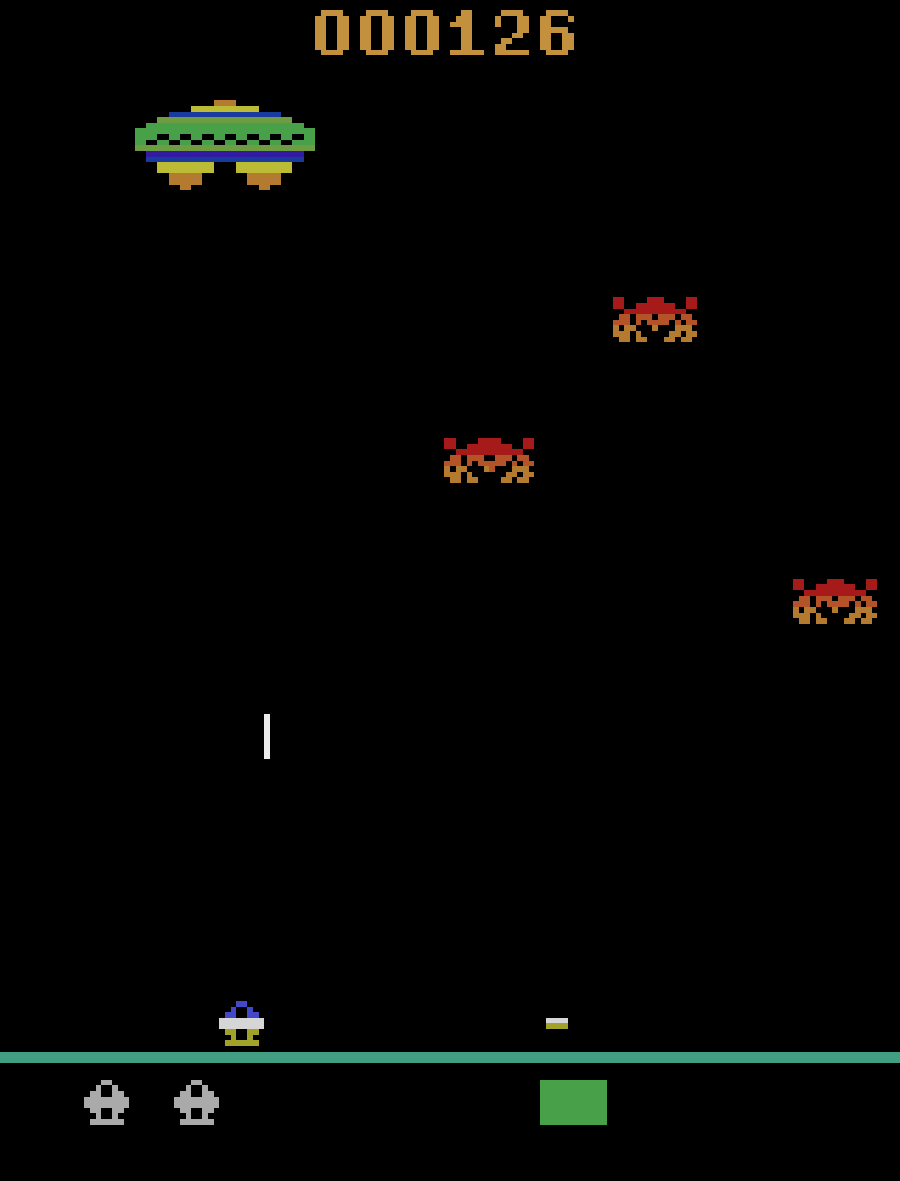
\includegraphics[width=0.3\linewidth]{img/assault_preview.png}
    \caption{Atari Assault environment.}
    \label{fig:assault_preview}
\end{figure}

For our modular framework, we break the objective down to a multi-objective problem, where each alien ship is viewed as a separate objective, and each local policy attempts to destroy its assigned target while avoiding enemy missiles. 
Not only does this facilitate an improvement in the performance, as we will demonstrate, but also we obtain a transparent design, because which target is being chased is revealed at each point. 
This modular design is made possible by the object-centric variant of the Atari environment \citep{delfosse2023ocatari}, which exposes the states of each individual target and the missiles by decoding the RAM states. 
The full observation space of each local policy also include the current position of the missile launcher, the current health, and the number of remaining lives. 
The local policy gets a reward or a penalty upon destroying its target enemy ship or losing a life, respectively. 
For local policy $i$, the Assault reward is
\[
    r_i =
    r_i^{\mathrm{destroy}}
    + r_i^{\mathrm{life}}
    + r_i^{\mathrm{overheat}}
    + r_i^{\mathrm{hot}}
    + r_i^{\mathrm{bid}}
    + r_i^{\mathrm{window}} .
\]
The destroy reward is credited to the policy assigned to the destroyed enemy, while life-loss, overheat, and fire-while-hot penalties discourage unsafe firing behavior.
The bid and action-window terms account for the auction mechanism.
Lastly, we use the game score as the metric for evaluation.
The Assault environment parameters are listed in~\Cref{tab:assault-env-params}, and the corresponding multi-policy, single-policy PPO, and DWN training parameters are listed in~\Cref{tab:assault-mappo-hparams,tab:assault-ppo-hparams,tab:assault-dwn-hparams}.

\textbf{Environment III: Atari Air-Raid.} Air-Raid uses the same modular Atari setup: each incoming enemy is treated as an objective and assigned to a local policy.
Positive score changes are interpreted as enemy kills, and each kill yields a destroy reward proportional to the score increase.
We also penalize near misses from enemy missiles: if an enemy missile enters a fixed box around the player without causing a life loss, the controlling policy receives a near-hit penalty.
For local policy $i$, the Air-Raid reward is
\[
    r_i =
    r_i^{\mathrm{destroy}}
    + r_i^{\mathrm{near\text{-}hit}}
    + r_i^{\mathrm{bid}} .
\]
Destroy rewards are credited to the policy associated with the hit enemy when that policy owns the player missile that caused the score event, near-hit penalties are assigned to the policy currently controlling the player, and bid penalties are applied according to the auction rule.
The single-policy PPO baseline uses the destroy and near-hit terms without bid penalties.
Additional training and implementation details are reported in~\Cref{sec:reprod-details}.


\textbf{Baseline approaches.}
We compare our method against two baselines: a single policy PPO with weighted rewards and deep W-learning (DWN; \citep{rosero2024multi}). 
For the original PPO baselines in the homogeneous environments, we use the total reward across objectives at each step.
We additionally evaluate urgency-weighted scalarization in Cat Feeder, where objective reward components are weighted dynamically by urgency.
The precise weighting and update order are given in Appendix~\ref{app:urgency-scalarization}.
We note that in Atari Assault and Air-raid, the single-policy PPO reward includes enemy-destroy rewards, raw score rewards, life-loss penalties, overheat penalties, and fire-while-hot penalties, but no bid or action-window terms.
The observation space remains the same as the multi-policy setting. 
In the Cat Feeder environment, we implement three reward mechanisms to help guide learning: one only with the sparse rewards from the environment, one with distance-based dense reward with respect to the nearest feeding request (denoted Nearest Shaping/NS in the experiments), and finally one where we provide distance-based reward with respect to the request that has the least amount of time until expiration (denoted Expiry Shaping/ES).
The single-policy PPO baseline does not use an action window: because there is no policy-switching decision, it selects a new action at every environment step. The action window \(\tau\) applies only to multi-policy methods, where it determines how long the selected local policy retains control after a bidding or W-network selection event.
The PPO implementation is taken from CleanRL~\citep{huang2022cleanrl}.
We use the specified PPO hyperparameters from CleanRL for the Atari games and we tune the hyperparameters for the Cat Feeder environment with 40 Optuna iterations~\citep{akiba2019optuna}.

DWN is another multi-policy method for multi-objective RL that uses DQN for each of the local policies and additionally learns a W-network for each policy that predict scalar weights. 
These weights are used to choose which policy's action should be played at each step. 
For temporal consistency among multi-policy methods, DWN uses the same action window \(\tau\) as our bidding methods.
The W-network is trained alongside the Q-network by updating it with a gradient step to predict the negative temporal difference (TD) error when the policy does not get to play its action.
The assertion here is that the negative TD-error quantifies how important it is for the policy to play its action. 
The implementation is borrowed from the repository of \citep{rosero2024multi}. All hyperparameters for the baselines are listed in~\Cref{sec:reprod-details}.

\textbf{Heterogeneous Cat Feeder.}
The extension adds priority-scaled feeding rewards and a distinct charging objective to the same gridworld.
Eight cat policies compete with one charging policy; the three charging stations and the cats move stochastically.
The charging policy has a battery-dependent effective bid boost to encode its known priority.
Battery dynamics, effective bids, network sharing, and the centralized reward are specified in Appendix~\ref{app:heterogeneous-implementation}.
The feeding metric sums priorities of completed requests (priorities 1--4), and battery depletions are reported separately.

\section{Additional Experimental Results}
\label{app:additional-experimental-results}

\begin{figure}[h]
    \centering
    \begin{subfigure}[t]{0.31\textwidth}
        \centering
        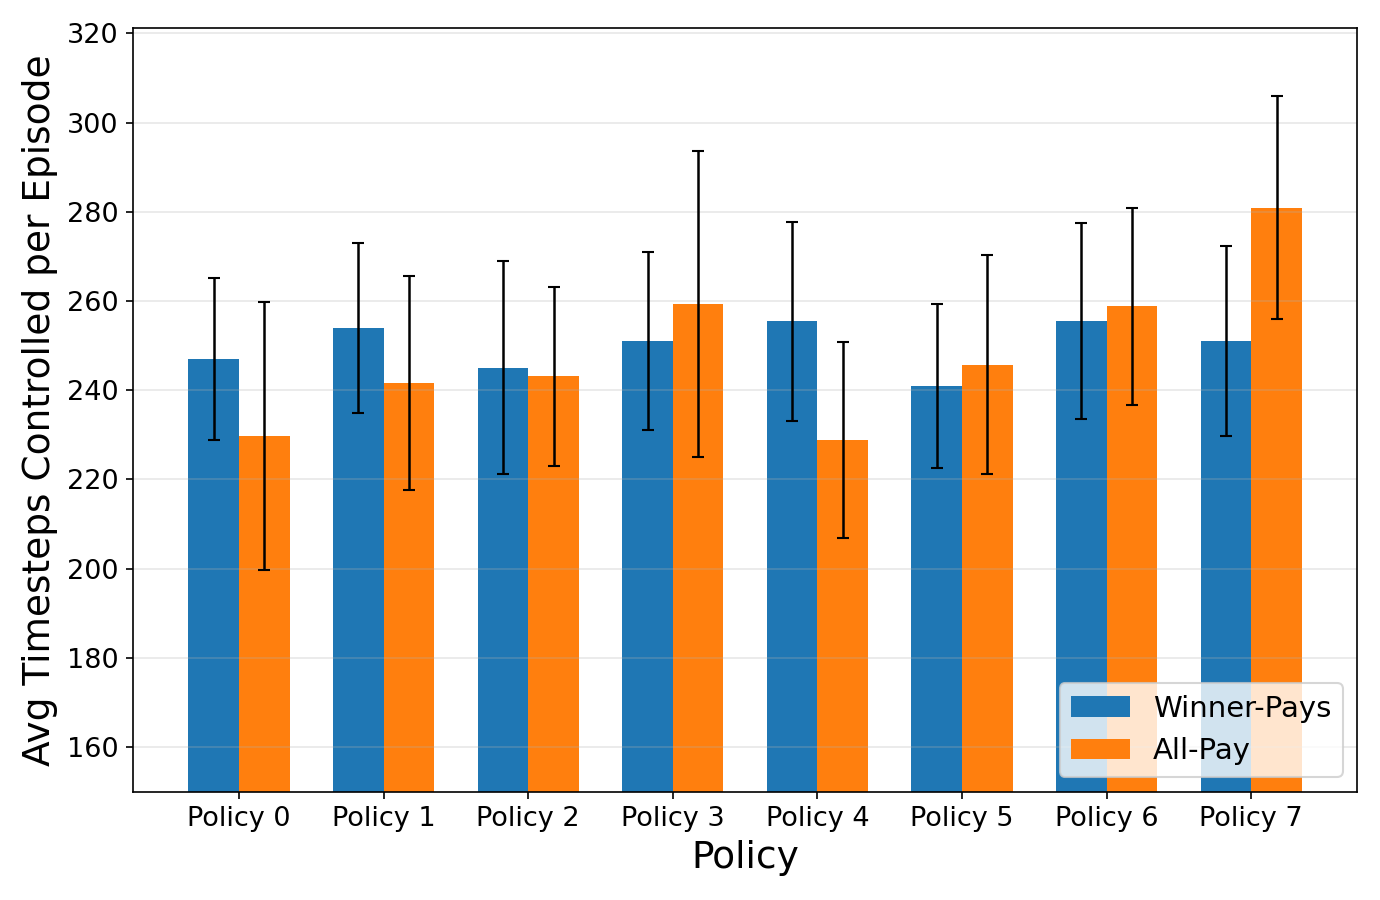
\includegraphics[width=\textwidth]{img/bidding_mechanisms_control_timesteps.png}
        \caption{Cat Feeder.}
        \label{fig:dyntar-control-dist}
    \end{subfigure}
    \hfill
    \begin{subfigure}[t]{0.25\textwidth}
        \centering
        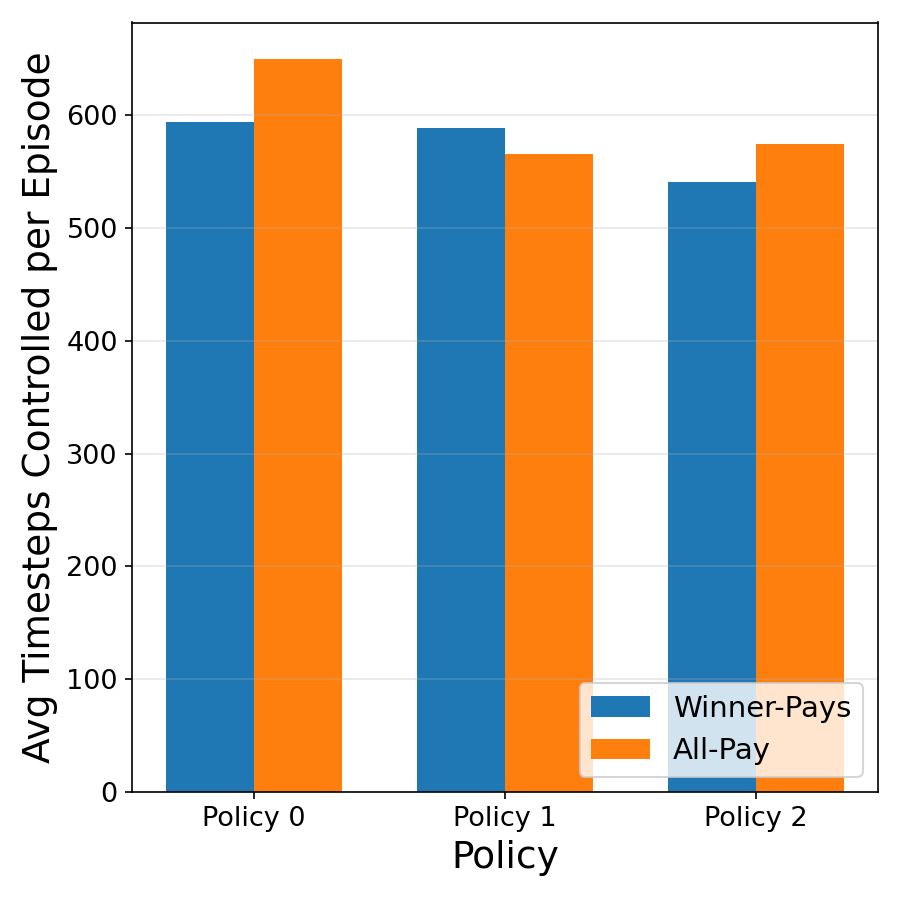
\includegraphics[width=\textwidth]{img/assault_bidding_mechanisms_control_timesteps.png}
        \caption{Atari Assault.}
        \label{fig:assault-control-dist}
    \end{subfigure}
    \hfill
    \begin{subfigure}[t]{0.25\textwidth}
        \centering
        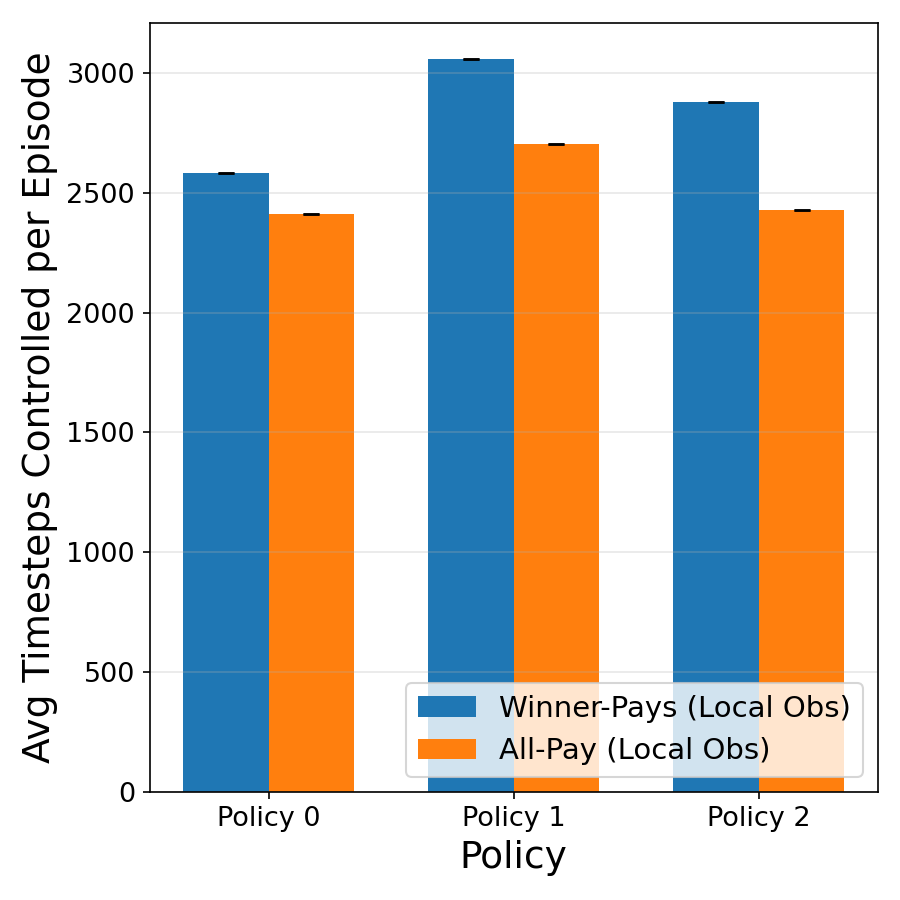
\includegraphics[width=\textwidth]{img/airraid_bidding_mechanisms_control_timesteps.png}
        \caption{Atari Air-Raid.}
        \label{fig:airraid-control-dist}
    \end{subfigure}
    \caption{Control distributions across environments and methods. The control distribution is the number of timesteps controlled by each policy.}
    \label{fig:control-dist-appendix}
\end{figure}

\begin{figure}[h]
    \centering
    \begin{subfigure}[b]{0.3\textwidth}
        \centering
        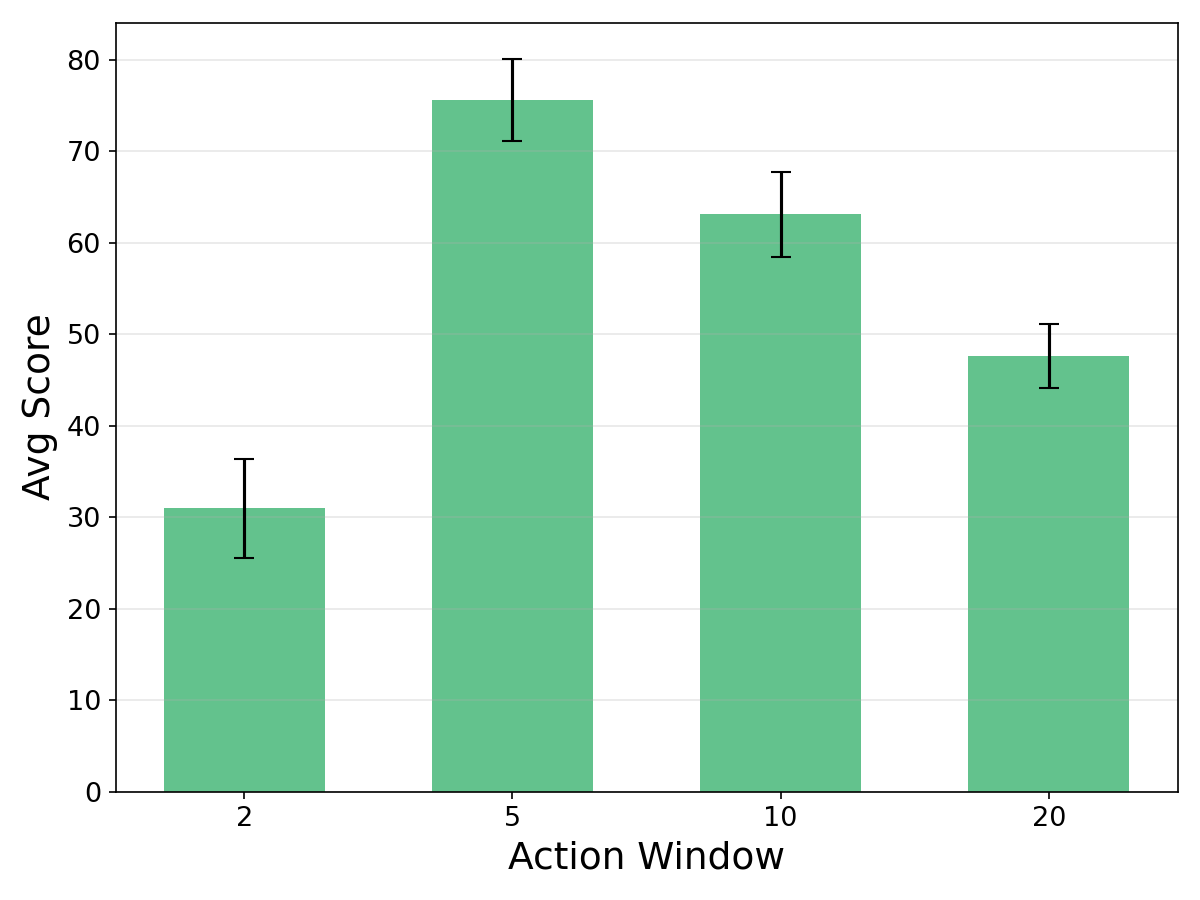
\includegraphics[width=\textwidth]{img/gridworld_action_window_bar_chart.png}
        \caption{Cat Feeder.}
    \end{subfigure}
    % \hfill
    \begin{subfigure}[b]{0.3\textwidth}
        \centering
        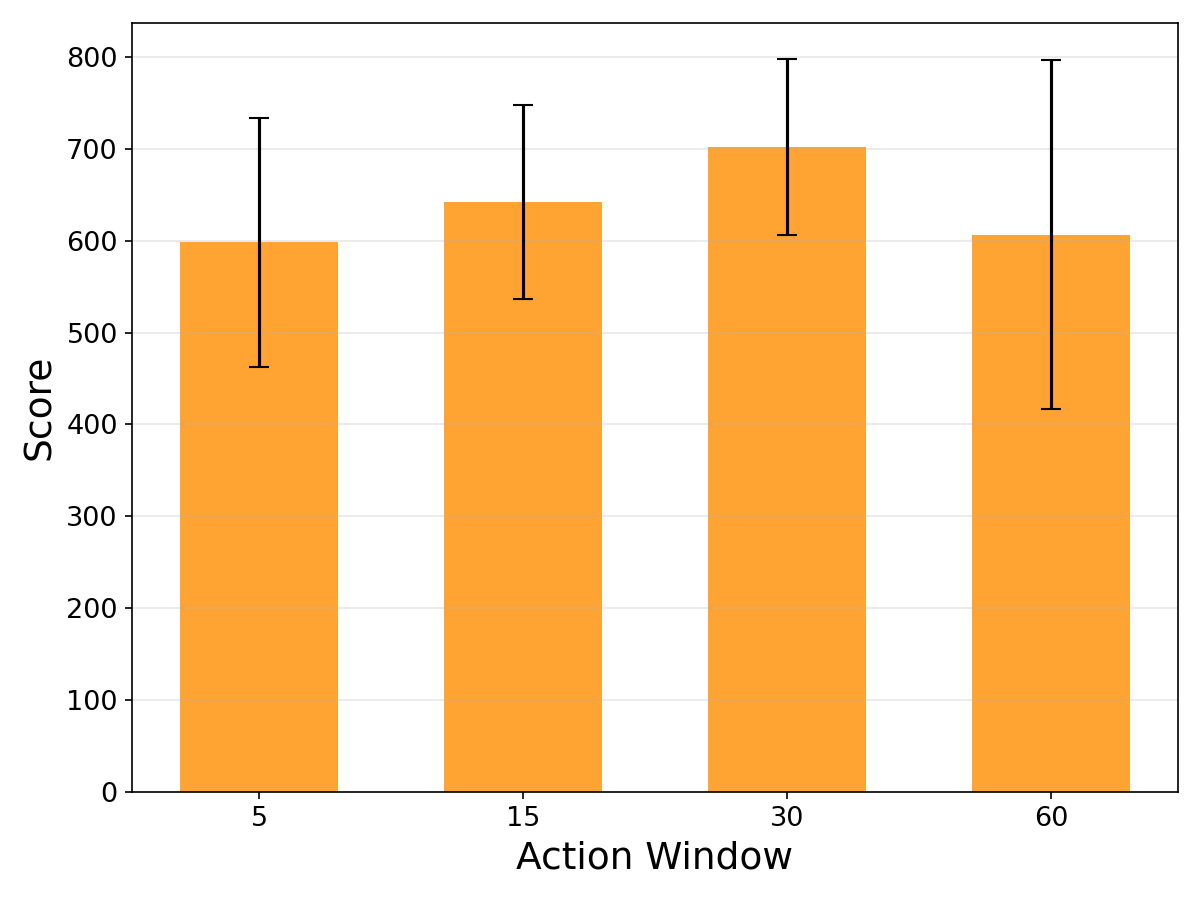
\includegraphics[width=\textwidth]{img/assault_action_window_bar_chart.png}
        \caption{Atari Assault.}
    \end{subfigure}
    \caption{Effect of the action-window size on performance.}
    \label{fig:action-window}
\end{figure}

\Cref{fig:action-window} studies the action-window size in the Cat Feeder and Atari Assault environments.
Smaller windows cause excessive switching between policies, while larger windows prevent sufficient switching to serve all objectives.
The best performance occurs at an intermediate action-window size.

\subsection{Heterogeneous Cat Feeder: Feeding Counts by Priority}
\label{app:heterogeneous-results}
Table~\ref{tab:priority-feeding-counts} breaks down completed feeding requests by priority in the heterogeneous environment.
The priority-weighted score in Table~\ref{tab:heterogeneous-cat-feeder} is the sum of these completion counts weighted by their priorities.
The results show service across all four priority levels while the charging policy competes for control.

\begin{table}[ht]
  \caption{Completed feeding requests by priority: mean (standard deviation). Priority 4 is the highest feeding priority.}
  \label{tab:priority-feeding-counts}
  \centering
  \begin{tabular}{lrrrr}
    \toprule
    Method & Priority 1 & Priority 2 & Priority 3 & Priority 4 \\
    \midrule
    All-Pay & $17.45\;(0.32)$ & $18.75\;(0.70)$ & $19.56\;(0.73)$ & $20.23\;(0.64)$ \\
    Centralized PPO & $6.82\;(1.55)$ & $8.61\;(3.12)$ & $11.72\;(6.13)$ & $13.17\;(7.77)$ \\
    \bottomrule
  \end{tabular}
\end{table}

\subsection{Target Coverage under Scaling}
\label{app:scaling-coverage}
Table~\ref{tab:scaling-coverage} reports the minimum per-target completion count when increasing the number of targets at deployment, averaged over twenty evaluation episodes.
For episode $e$ and target $i$, let $C_{e,i}$ be its completion count.
The reported statistic is
\begin{equation}
  \overline C_{\min}=\frac{1}{E}\sum_{e=1}^{E}\min_i C_{e,i},
  \qquad E=20.
\end{equation}
The minimum is taken within each episode before averaging, rather than taking the minimum of per-target episode averages.
These values are read from the saved JSON field \texttt{statistics.avg\_min\_targets\_reached} and recompute from the twenty episode-level minima.
Scaling selects the single periodic checkpoint with the highest \texttt{avg\_avg\_performance}, as detailed in Appendix~\ref{app:evaluation-aggregation}.
The model is trained with eight targets and transferred by adding copies of the learned policy, each conditioned on its assigned target.
The episode length remains fixed, so additional targets divide the available service time and may expire before being reached.
Positive coverage at every tested size indicates that no target is entirely excluded in this aggregate, but does not imply equal service or invariant performance.

\begin{table}[ht]
  \caption{Scaling Cat Feeder: mean of the per-episode minimum target-completion counts across twenty episodes.}
  \label{tab:scaling-coverage}
  \centering
  \begin{tabular}{lrrrr}
    \toprule
    Number of targets & 8 & 10 & 12 & 14 \\
    \midrule
    Minimum completion count & 8.2 & 5.7 & 5.9 & 4.1 \\
    \bottomrule
  \end{tabular}
\end{table}

\section{Additional Implementation Details}
\label{app:additional-implementation-details}

\subsection{Parameter Sharing}
\label{app:parameter-sharing}

In our homogeneous-objective experiments, the objectives are symmetric: each local policy solves the same type of reachability task, but for a different assigned target. We therefore share the actor-critic network parameters across local policies. This reduces the number of learned parameters and lets the shared network receive PPO updates from all local-policy objectives.

Parameter sharing does not make the local policies indistinguishable. For each local policy \(i\), the policy input contains both a pooled embedding of the full set of objective vectors and the objective-specific vector \(z_i\) for that policy's assigned target. Thus two policy copies share network weights, but are conditioned on different \(z_i\)'s and receive different local rewards. In Cat Feeder, \(z_i\) encodes the assigned feeding request, including its position and remaining lifetime; in the Atari environments, \(z_i\) encodes the assigned enemy object exposed by the object-centric observation.

\subsection{Urgency-Weighted Scalarization}
\label{app:urgency-scalarization}
Let $L$ denote the target expiry interval (\texttt{target\_expiry\_steps}), distinct from the episode horizon $H$, and let $c_{i,t}$ be target $i$'s age counter in the state before action $t$.
Define its clamped remaining lifetime, urgency, and normalized weight by
\begin{align}
  \ell_{i,t} &= \max\{L-c_{i,t},1\}, &
  q_{i,t} &= \frac{\mathbf{1}[i\text{ active at }t]}{\ell_{i,t}}, \\
  w_{i,t} &=
  \begin{cases}
    q_{i,t}/\sum_j q_{j,t}, & \sum_j q_{j,t}>0,\\
    0, & \text{otherwise}.
  \end{cases}
\end{align}
The weights are computed before movement, counter increments, expiration, or respawn.
Active weights sum to one, reached static targets receive zero weight, and there is no additional normalization by the number of targets.
For example, two active targets with remaining lifetimes 1 and 4 receive weights $0.8$ and $0.2$.
The scalar reward is
\begin{equation}
  r_t = \sum_i w_{i,t} r^{\mathrm{obj}}_{i,t}
        -\lambda_B\mathbf{1}[\text{battery depletion at }t],
\end{equation}
where $r^{\mathrm{obj}}_{i,t}$ includes distance-improvement shaping, priority-weighted completion reward, and the expiry penalty.
The depletion term applies only in battery-enabled environments and is not multiplied by target urgency weights.

\subsection{Heterogeneous Cat Feeder Implementation}
\label{app:heterogeneous-implementation}
\paragraph{Battery and stations.}
The reported moving-station comparison uses battery capacity 50.
The three stations start at $(0,0)$, $(15,15)$, and $(29,29)$ and follow independent bounded persistent random walks, moving every 15 steps with direction-change probability $0.1$.
A successful one-cell movement consumes one battery unit; boundary or no-movement steps consume none.
Occupying a charging station immediately restores the battery to capacity.
Reaching zero away from a station causes an immediate tow to the nearest station and a full refill; we count such events as battery depletions.
A capacity-40 fixed-station reference configuration is a different benchmark and is not the configuration used for the reported moving-station results.

\paragraph{Effective bids and payments.}
Feeders and charger both choose raw categorical bids in $\{0,\ldots,6\}$.
Let $B_t$ be the current battery level and $e_t$ the energy required to reach the nearest station.
The charger is forced to bid zero unless $B_t\leq e_t+8$.
For a permitted raw charger bid $b_{\mathrm{chg},t}$, the bid used to determine the winner is
\begin{equation}
  b^{\mathrm{eff}}_{\mathrm{chg},t}
  = b_{\mathrm{chg},t}
    +2\mathbf{1}[b_{\mathrm{chg},t}>0\ \land\ B_t\leq25].
\end{equation}
Thus the effective charger ceiling is 8 when the boost applies, versus 6 for feeders.
The All-Pay payment uses the raw bid, not the boosted effective bid.
This battery-dependent priority rule is an implementation extension to the common-cap auction analyzed in the theory.

\paragraph{Parameter sharing.}
The eight feeder controllers share one actor--critic network, with observations reordered according to the assigned target identity.
The charger uses a completely separate actor--critic with separate direction and bid actor trunks in the moving-station experiment.
No parameters are shared between feeders and charger.

\paragraph{Centralized baseline.}
The unassisted centralized PPO baseline in Table~\ref{tab:heterogeneous-cat-feeder} directly chooses body movement without bidding, an action window, or an execution-time action override.
Let $d_{i,t}$ be distance to target $i$, $p_i\in\{1,2,3,4\}$ its feeding priority, and $D_t$ the battery-depletion indicator.
Its unweighted scalar reward is
\begin{equation}
\begin{split}
 r_t={}&\sum_i\bigl[0.6(d_{i,t}-d_{i,t+1})
       +20p_i\mathbf{1}[i\text{ reached at }t]\\
       &\hspace{3em}-50\mathbf{1}[i\text{ expired at }t]\bigr]-10D_t.
\end{split}
\end{equation}
An assisted centralized variant adds reserve-gated progress shaping toward a station, a refill bonus proportional to the restored battery fraction, and an additional depletion penalty of $100$.
It also has no execution-time action override; these auxiliary terms are not part of the unassisted baseline reported here.

\subsection{Evaluation Aggregation}
\label{app:evaluation-aggregation}
For Table~\ref{tab:all_methods_comp}, PPO results first average each seed's last five available evaluation checkpoints, then report the mean and sample standard deviation across seed averages.
The local-observation ablation (\texttt{visible\_targets=0}, called blind in the discussion) uses the same aggregation as the other PPO variants.
Scaling evaluations use a different checkpoint-selection procedure: a single periodic checkpoint is selected by the largest \texttt{avg\_avg\_performance}, rather than averaging the final five checkpoints.
This selection uses evaluation performance and should be distinguished from evaluating a prespecified final checkpoint on an independent test set.
The scaling plot displays eight times the mean per-episode average performance, which is distinct from the minimum-completion statistic defined in Appendix~\ref{app:scaling-coverage}.

% ============================================================
\section{Reproducibility Details}
\label{sec:reprod-details}
% ============================================================

The code for all experiments is included in the supplementary materials.

All experiments use 10 random seeds: \{1825, 410, 4507, 4013, 3658, 5215, 6861, 6803, 7819, 8057\}.

\paragraph{Existing assets and licenses.}
Our experiments use the Arcade Learning Environment (ALE)~\citep{bellemare13arcade}, OCAtari~\citep{delfosse2023ocatari}, CleanRL~\citep{huang2022cleanrl}, Optuna~\citep{akiba2019optuna}, and the Deep W-Learning implementation associated with~\citet{rosero2024multi}. We use these assets only for research experiments and cite their original sources. The corresponding software licenses and terms of use are those distributed with the respective public repositories; we include the exact versions, repository URLs, and license names in the released supplementary code.

% ============================================================
\subsection{Cat Feeder Environment}
% ============================================================

\begin{table}[h]
\caption{Cat Feeder shared (training) environment parameters.}
\label{tab:cat-feeder-env-params}
\centering
\begin{tabular}{ll}
\toprule
Parameter & Value \\
\midrule
Grid size & $30 \times 30$ \\
Number of agents / targets & 8 \\
Target reward & 50.0 \\
Target expiry steps & 200 \\
Target expiry penalty & 50.0 \\
Max episode steps & 2000 \\
Moving targets & True \\
Direction change probability & 0.1 \\
Target move interval & 5 \\
\bottomrule
\end{tabular}
\end{table}

\begin{table}[h]
\caption{Cat Feeder multi-agent PPO hyperparameters (\allpay and \poorman).}
\label{tab:cat-feeder-mappo-hparams}
\centering
\begin{tabular}{ll}
\toprule
Parameter & Value \\
\midrule
\multicolumn{2}{l}{\textit{Auction}} \\
Bid upper bound & 6 \\
Bid penalty & 0.1 \\
Action window & 5 \\
Distance reward scale & 0.6 \\
\midrule
\multicolumn{2}{l}{\textit{Training}} \\
Iterations & 400 \\
Parallel environments & 4096 \\
Steps per rollout & 256 \\
Minibatches & 256 \\
PPO epochs & 4 \\
Learning rate & $2.5 \times 10^{-4}$ (annealed) \\
Discount $\gamma$ & 0.99 \\
GAE $\lambda$ & 0.95 \\
Clip coefficient & 0.05 \\
Entropy coefficient & 0.03 \\
Value function coefficient & 1.0 \\
Max gradient norm & 0.5 \\
\midrule
\multicolumn{2}{l}{\textit{Network}} \\
Actor hidden layers & $[128, 128, 128, 128]$ \\
Critic hidden layers & $[256, 256, 256, 256]$ \\
Target attention pooling & True \\
Target embedding dim & 64 \\
Target encoder hidden layers & $[64, 64]$ \\
\bottomrule
\end{tabular}
\end{table}

\begin{table}[h]
\caption{Cat Feeder single-agent PPO baseline hyperparameters. Hyperparameters were tuned using Optuna with 40 trials. The nearest-target shaping variant is identical but uses a distance reward scale of 0.6 with shaping toward the nearest target.}
\label{tab:cat-feeder-ppo-hparams}
\centering
\begin{tabular}{ll}
\toprule
Parameter & Value \\
\midrule
\multicolumn{2}{l}{\textit{Training}} \\
Iterations & 400 \\
Parallel environments & 4096 \\
Steps per rollout & 256 \\
Minibatches & 512 \\
PPO epochs & 8 \\
Learning rate & $1.74 \times 10^{-4}$ (annealed) \\
Discount $\gamma$ & 0.963 \\
GAE $\lambda$ & 0.970 \\
Clip coefficient & 0.327 \\
Entropy coefficient & $1.03 \times 10^{-4}$ \\
Value function coefficient & 1.076 \\
Max gradient norm & 0.840 \\
Distance reward scale & 0.0 \\
Target attention pooling & False \\
\midrule
\multicolumn{2}{l}{\textit{Network (shared with multi-agent PPO)}} \\
Actor hidden layers & $[128, 128, 128, 128]$ \\
Critic hidden layers & $[256, 256, 256, 256]$ \\
\bottomrule
\end{tabular}
\end{table}

\begin{table}[h]
\caption{Cat Feeder DWN baseline hyperparameters.}
\label{tab:cat-feeder-dwn-hparams}
\centering
\begin{tabular}{ll}
\toprule
Parameter & Value \\
\midrule
\multicolumn{2}{l}{\textit{Training}} \\
Total timesteps & $5 \times 10^{8}$ \\
Parallel environments & 256 \\
Discount $\gamma$ & 0.99 \\
Replay buffer size & $1 \times 10^{6}$ \\
Batch size & 256 \\
Learning starts & $1 \times 10^{5}$ \\
Train frequency & 256 \\
W-network train delay & $1 \times 10^{6}$ \\
Target network update frequency & 1000 \\
Target network $\tau$ & 1.0 \\
\midrule
\multicolumn{2}{l}{\textit{Networks}} \\
Q-network hidden layers & $[256, 256, 256, 256]$ \\
W-network hidden layers & $[128, 128, 128]$ \\
Q-network learning rate & $1 \times 10^{-4}$ \\
W-network learning rate & $1 \times 10^{-4}$ \\
\midrule
\multicolumn{2}{l}{\textit{Epsilon schedules}} \\
Q $\varepsilon$ start / min / decay & 0.99 / 0.01 / 0.99 \\
W $\varepsilon$ start / min / decay & 0.99 / 0.01 / 0.99 \\
\bottomrule
\end{tabular}
\end{table}

% ============================================================
\subsection{Assault Environment}
% ============================================================

\begin{table}[h]
\caption{Assault shared environment parameters.}
\label{tab:assault-env-params}
\centering
\begin{tabular}{ll}
\toprule
Parameter & Value \\
\midrule
Number of agents & 3 \\
Max enemies & 3 \\
Max episode steps & 10000 \\
Enemy destroy reward & 10.0 \\
Life loss penalty & 10.0 \\
Fire-while-hot penalty & 8.0 \\
Action window & 15 \\
Bid upper bound & 2 \\
Bid penalty & 0.3 \\
\bottomrule
\end{tabular}
\end{table}

\begin{table}[h]
\caption{Assault multi-agent PPO hyperparameters (\allpay and \poorman).}
\label{tab:assault-mappo-hparams}
\centering
\begin{tabular}{ll}
\toprule
Parameter & Value \\
\midrule
\multicolumn{2}{l}{\textit{Training}} \\
Iterations & 150 \\
Parallel environments & 128 \\
Steps per rollout & 512 \\
Minibatches & 8 \\
PPO epochs & 8 \\
Learning rate & $1 \times 10^{-4}$ (annealed) \\
Discount $\gamma$ & 0.99 \\
GAE $\lambda$ & 0.95 \\
Clip coefficient & 0.05 \\
Entropy coefficient & 0.05 \\
Value function coefficient & 0.5 \\
Max gradient norm & 0.5 \\
Target KL & 0.02 \\
\midrule
\multicolumn{2}{l}{\textit{Network}} \\
Actor hidden layers & $[128, 128, 128, 128]$ \\
Critic hidden layers & $[256, 256, 256, 256]$ \\
\bottomrule
\end{tabular}
\end{table}

\begin{table}[h]
\caption{Assault single-agent PPO baseline hyperparameters (differences from multi-agent PPO only; all other parameters are shared).}
\label{tab:assault-ppo-hparams}
\centering
\begin{tabular}{ll}
\toprule
Parameter & Value \\
\midrule
Learning rate & $2.5 \times 10^{-4}$ (annealed) \\
Clip coefficient & 0.1 \\
Entropy coefficient & 0.01 \\
Target KL & --- \\
\bottomrule
\end{tabular}
\end{table}

\begin{table}[h]
\caption{Assault DWN baseline hyperparameters.}
\label{tab:assault-dwn-hparams}
\centering
\begin{tabular}{ll}
\toprule
Parameter & Value \\
\midrule
\multicolumn{2}{l}{\textit{Training}} \\
Total timesteps & $1 \times 10^{7}$ \\
Parallel environments & 8 \\
Discount $\gamma$ & 0.99 \\
Replay buffer size & $5 \times 10^{5}$ \\
Batch size & 256 \\
Learning starts & $1 \times 10^{4}$ \\
Train frequency & 80 \\
W-network train delay & $1 \times 10^{5}$ \\
Target network update frequency & 1000 \\
Target network $\tau$ & 1.0 \\
\midrule
\multicolumn{2}{l}{\textit{Networks}} \\
Q-network hidden layers & $[256, 256, 256]$ \\
W-network hidden layers & $[128, 128, 128]$ \\
Q-network learning rate & $1 \times 10^{-4}$ \\
W-network learning rate & $1 \times 10^{-4}$ \\
\midrule
\multicolumn{2}{l}{\textit{Epsilon schedules}} \\
Q $\varepsilon$ start / min / decay & 0.99 / 0.01 / 0.995 \\
W $\varepsilon$ start / min / decay & 0.99 / 0.01 / 0.995 \\
\bottomrule
\end{tabular}
\end{table}

%%%%%%%%%%%%%%%%%%%%%%%%%%%%%%%%%%%%%%%%%%%%%%%%%%%%%%%%%%%%

\clearpage
\section*{NeurIPS Paper Checklist}

\begin{enumerate}

\item {\bf Claims}
    \item[] Question: Do the main claims made in the abstract and introduction accurately reflect the paper's contributions and scope?
    \item[] Answer: \answerYes{}
    \item[] Justification: The abstract and introduction state the paper's main contribution: an auction-based framework for adapting among local policies in multi-objective RL. The experimental claims are supported in Section~\ref{sec:experimental-results}, with scope and future directions discussed in the conclusion.
    \item[] Guidelines:
    \begin{itemize}
        \item The answer \answerNA{} means that the abstract and introduction do not include the claims made in the paper.
        \item The abstract and/or introduction should clearly state the claims made, including the contributions made in the paper and important assumptions and limitations. A \answerNo{} or \answerNA{} answer to this question will not be perceived well by the reviewers. 
        \item The claims made should match theoretical and experimental results, and reflect how much the results can be expected to generalize to other settings. 
        \item It is fine to include aspirational goals as motivation as long as it is clear that these goals are not attained by the paper. 
    \end{itemize}

\item {\bf Limitations}
    \item[] Question: Does the paper discuss the limitations of the work performed by the authors?
    \item[] Answer: \answerYes{}
    \item[] Justification: The conclusion discusses current scope limitations, including explicit objective decomposition, the scope of shared-policy transfer, limited experimental breadth, and the absence of safety guarantees in the heterogeneous feeding-and-charging experiment.
    \item[] Guidelines:
    \begin{itemize}
        \item The answer \answerNA{} means that the paper has no limitation while the answer \answerNo{} means that the paper has limitations, but those are not discussed in the paper. 
        \item The authors are encouraged to create a separate ``Limitations'' section in their paper.
        \item The paper should point out any strong assumptions and how robust the results are to violations of these assumptions (e.g., independence assumptions, noiseless settings, model well-specification, asymptotic approximations only holding locally). The authors should reflect on how these assumptions might be violated in practice and what the implications would be.
        \item The authors should reflect on the scope of the claims made, e.g., if the approach was only tested on a few datasets or with a few runs. In general, empirical results often depend on implicit assumptions, which should be articulated.
        \item The authors should reflect on the factors that influence the performance of the approach. For example, a facial recognition algorithm may perform poorly when image resolution is low or images are taken in low lighting. Or a speech-to-text system might not be used reliably to provide closed captions for online lectures because it fails to handle technical jargon.
        \item The authors should discuss the computational efficiency of the proposed algorithms and how they scale with dataset size.
        \item If applicable, the authors should discuss possible limitations of their approach to address problems of privacy and fairness.
        \item While the authors might fear that complete honesty about limitations might be used by reviewers as grounds for rejection, a worse outcome might be that reviewers discover limitations that aren't acknowledged in the paper. The authors should use their best judgment and recognize that individual actions in favor of transparency play an important role in developing norms that preserve the integrity of the community. Reviewers will be specifically instructed to not penalize honesty concerning limitations.
    \end{itemize}

\item {\bf Theory assumptions and proofs}
    \item[] Question: For each theoretical result, does the paper provide the full set of assumptions and a complete (and correct) proof?
    \item[] Answer: \answerYes{}
    \item[] Justification: The theoretical results in Section~\ref{sec:auction-framework} state the assumptions for the bidding settings and include proofs in the main text.
    \item[] Guidelines:
    \begin{itemize}
        \item The answer \answerNA{} means that the paper does not include theoretical results. 
        \item All the theorems, formulas, and proofs in the paper should be numbered and cross-referenced.
        \item All assumptions should be clearly stated or referenced in the statement of any theorems.
        \item The proofs can either appear in the main paper or the supplemental material, but if they appear in the supplemental material, the authors are encouraged to provide a short proof sketch to provide intuition. 
        \item Inversely, any informal proof provided in the core of the paper should be complemented by formal proofs provided in appendix or supplemental material.
        \item Theorems and Lemmas that the proof relies upon should be properly referenced. 
    \end{itemize}

    \item {\bf Experimental result reproducibility}
    \item[] Question: Does the paper fully disclose all the information needed to reproduce the main experimental results of the paper to the extent that it affects the main claims and/or conclusions of the paper (regardless of whether the code and data are provided or not)?
    \item[] Answer: \answerYes{}
    \item[] Justification: Section~\ref{sec:experimental-results} describes the environments, baselines, ablations, and evaluation protocol, while Appendix~\ref{sec:reprod-details} provides seeds and hyperparameters needed to reproduce the main experiments.
    \item[] Guidelines:
    \begin{itemize}
        \item The answer \answerNA{} means that the paper does not include experiments.
        \item If the paper includes experiments, a \answerNo{} answer to this question will not be perceived well by the reviewers: Making the paper reproducible is important, regardless of whether the code and data are provided or not.
        \item If the contribution is a dataset and\slash or model, the authors should describe the steps taken to make their results reproducible or verifiable. 
        \item Depending on the contribution, reproducibility can be accomplished in various ways. For example, if the contribution is a novel architecture, describing the architecture fully might suffice, or if the contribution is a specific model and empirical evaluation, it may be necessary to either make it possible for others to replicate the model with the same dataset, or provide access to the model. In general. releasing code and data is often one good way to accomplish this, but reproducibility can also be provided via detailed instructions for how to replicate the results, access to a hosted model (e.g., in the case of a large language model), releasing of a model checkpoint, or other means that are appropriate to the research performed.
        \item While NeurIPS does not require releasing code, the conference does require all submissions to provide some reasonable avenue for reproducibility, which may depend on the nature of the contribution. For example
        \begin{enumerate}
            \item If the contribution is primarily a new algorithm, the paper should make it clear how to reproduce that algorithm.
            \item If the contribution is primarily a new model architecture, the paper should describe the architecture clearly and fully.
            \item If the contribution is a new model (e.g., a large language model), then there should either be a way to access this model for reproducing the results or a way to reproduce the model (e.g., with an open-source dataset or instructions for how to construct the dataset).
            \item We recognize that reproducibility may be tricky in some cases, in which case authors are welcome to describe the particular way they provide for reproducibility. In the case of closed-source models, it may be that access to the model is limited in some way (e.g., to registered users), but it should be possible for other researchers to have some path to reproducing or verifying the results.
        \end{enumerate}
    \end{itemize}


\item {\bf Open access to data and code}
    \item[] Question: Does the paper provide open access to the data and code, with sufficient instructions to faithfully reproduce the main experimental results, as described in supplemental material?
    \item[] Answer: \answerYes{}
    \item[] Justification: The supplementary material includes the codebase and recorded rollouts, and Appendix~\ref{sec:reprod-details} reports the seeds and experiment hyperparameters.
    \item[] Guidelines:
    \begin{itemize}
        \item The answer \answerNA{} means that paper does not include experiments requiring code.
        \item Please see the NeurIPS code and data submission guidelines (\url{https://neurips.cc/public/guides/CodeSubmissionPolicy}) for more details.
        \item While we encourage the release of code and data, we understand that this might not be possible, so \answerNo{} is an acceptable answer. Papers cannot be rejected simply for not including code, unless this is central to the contribution (e.g., for a new open-source benchmark).
        \item The instructions should contain the exact command and environment needed to run to reproduce the results. See the NeurIPS code and data submission guidelines (\url{https://neurips.cc/public/guides/CodeSubmissionPolicy}) for more details.
        \item The authors should provide instructions on data access and preparation, including how to access the raw data, preprocessed data, intermediate data, and generated data, etc.
        \item The authors should provide scripts to reproduce all experimental results for the new proposed method and baselines. If only a subset of experiments are reproducible, they should state which ones are omitted from the script and why.
        \item At submission time, to preserve anonymity, the authors should release anonymized versions (if applicable).
        \item Providing as much information as possible in supplemental material (appended to the paper) is recommended, but including URLs to data and code is permitted.
    \end{itemize}


\item {\bf Experimental setting/details}
    \item[] Question: Does the paper specify all the training and test details (e.g., data splits, hyperparameters, how they were chosen, type of optimizer) necessary to understand the results?
    \item[] Answer: \answerYes{}
    \item[] Justification: Section~\ref{sec:experimental-results} summarizes the experimental setup, environments, baselines, and evaluation metrics. Appendix~\ref{sec:reprod-details} lists the environment parameters, PPO/DWN hyperparameters, random seeds, and tuning details.
    \item[] Guidelines:
    \begin{itemize}
        \item The answer \answerNA{} means that the paper does not include experiments.
        \item The experimental setting should be presented in the core of the paper to a level of detail that is necessary to appreciate the results and make sense of them.
        \item The full details can be provided either with the code, in appendix, or as supplemental material.
    \end{itemize}

\item {\bf Experiment statistical significance}
    \item[] Question: Does the paper report error bars suitably and correctly defined or other appropriate information about the statistical significance of the experiments?
    \item[] Answer: \answerYes{}
    \item[] Justification: The learning curves in Figure~\ref{fig:learning-curves} report the mean over 10 random seeds with shaded regions corresponding to one standard deviation.
    \item[] Guidelines:
    \begin{itemize}
        \item The answer \answerNA{} means that the paper does not include experiments.
        \item The authors should answer \answerYes{} if the results are accompanied by error bars, confidence intervals, or statistical significance tests, at least for the experiments that support the main claims of the paper.
        \item The factors of variability that the error bars are capturing should be clearly stated (for example, train/test split, initialization, random drawing of some parameter, or overall run with given experimental conditions).
        \item The method for calculating the error bars should be explained (closed form formula, call to a library function, bootstrap, etc.)
        \item The assumptions made should be given (e.g., Normally distributed errors).
        \item It should be clear whether the error bar is the standard deviation or the standard error of the mean.
        \item It is OK to report 1-sigma error bars, but one should state it. The authors should preferably report a 2-sigma error bar than state that they have a 96\% CI, if the hypothesis of Normality of errors is not verified.
        \item For asymmetric distributions, the authors should be careful not to show in tables or figures symmetric error bars that would yield results that are out of range (e.g., negative error rates).
        \item If error bars are reported in tables or plots, the authors should explain in the text how they were calculated and reference the corresponding figures or tables in the text.
    \end{itemize}

\item {\bf Experiments compute resources}
    \item[] Question: For each experiment, does the paper provide sufficient information on the computer resources (type of compute workers, memory, time of execution) needed to reproduce the experiments?
    \item[] Answer: \answerNo{}
    \item[] Justification: The paper reports the hardware configuration, training lengths, rollout sizes, numbers of parallel environments, and other computational parameters in Appendix~\ref{sec:reprod-details}. Wall-clock execution time and total compute budget were not recorded.
    \item[] Guidelines:
    \begin{itemize}
        \item The answer \answerNA{} means that the paper does not include experiments.
        \item The paper should indicate the type of compute workers CPU or GPU, internal cluster, or cloud provider, including relevant memory and storage.
        \item The paper should provide the amount of compute required for each of the individual experimental runs as well as estimate the total compute. 
        \item The paper should disclose whether the full research project required more compute than the experiments reported in the paper (e.g., preliminary or failed experiments that didn't make it into the paper). 
    \end{itemize}
    
\item {\bf Code of ethics}
    \item[] Question: Does the research conducted in the paper conform, in every respect, with the NeurIPS Code of Ethics \url{https://neurips.cc/public/EthicsGuidelines}?
    \item[] Answer: \answerYes{}
    \item[] Justification: The work uses simulated reinforcement-learning environments and does not involve human subjects, private data, or deployed systems. We are not aware of any aspect of the research that conflicts with the NeurIPS Code of Ethics.
    \item[] Guidelines:
    \begin{itemize}
        \item The answer \answerNA{} means that the authors have not reviewed the NeurIPS Code of Ethics.
        \item If the authors answer \answerNo, they should explain the special circumstances that require a deviation from the Code of Ethics.
        \item The authors should make sure to preserve anonymity (e.g., if there is a special consideration due to laws or regulations in their jurisdiction).
    \end{itemize}


\item {\bf Broader impacts}
    \item[] Question: Does the paper discuss both potential positive societal impacts and negative societal impacts of the work performed?
    \item[] Answer: \answerNA{}
    \item[] Justification: The paper is primarily methodological and experimental, and no deployment or human-facing application is studied.
    \item[] Guidelines:
    \begin{itemize}
        \item The answer \answerNA{} means that there is no societal impact of the work performed.
        \item If the authors answer \answerNA{} or \answerNo, they should explain why their work has no societal impact or why the paper does not address societal impact.
        \item Examples of negative societal impacts include potential malicious or unintended uses (e.g., disinformation, generating fake profiles, surveillance), fairness considerations (e.g., deployment of technologies that could make decisions that unfairly impact specific groups), privacy considerations, and security considerations.
        \item The conference expects that many papers will be foundational research and not tied to particular applications, let alone deployments. However, if there is a direct path to any negative applications, the authors should point it out. For example, it is legitimate to point out that an improvement in the quality of generative models could be used to generate Deepfakes for disinformation. On the other hand, it is not needed to point out that a generic algorithm for optimizing neural networks could enable people to train models that generate Deepfakes faster.
        \item The authors should consider possible harms that could arise when the technology is being used as intended and functioning correctly, harms that could arise when the technology is being used as intended but gives incorrect results, and harms following from (intentional or unintentional) misuse of the technology.
        \item If there are negative societal impacts, the authors could also discuss possible mitigation strategies (e.g., gated release of models, providing defenses in addition to attacks, mechanisms for monitoring misuse, mechanisms to monitor how a system learns from feedback over time, improving the efficiency and accessibility of ML).
    \end{itemize}
    
\item {\bf Safeguards}
    \item[] Question: Does the paper describe safeguards that have been put in place for responsible release of data or models that have a high risk for misuse (e.g., pre-trained language models, image generators, or scraped datasets)?
    \item[] Answer: \answerNA{}
    \item[] Justification: The paper does not release high-risk generative models, scraped datasets, or other assets with an apparent high risk of misuse.
    \item[] Guidelines:
    \begin{itemize}
        \item The answer \answerNA{} means that the paper poses no such risks.
        \item Released models that have a high risk for misuse or dual-use should be released with necessary safeguards to allow for controlled use of the model, for example by requiring that users adhere to usage guidelines or restrictions to access the model or implementing safety filters. 
        \item Datasets that have been scraped from the Internet could pose safety risks. The authors should describe how they avoided releasing unsafe images.
        \item We recognize that providing effective safeguards is challenging, and many papers do not require this, but we encourage authors to take this into account and make a best faith effort.
    \end{itemize}

\item {\bf Licenses for existing assets}
    \item[] Question: Are the creators or original owners of assets (e.g., code, data, models), used in the paper, properly credited and are the license and terms of use explicitly mentioned and properly respected?
    \item[] Answer: \answerYes{}
    \item[] Justification: Appendix~\ref{sec:reprod-details} credits the existing assets used in the experiments, cites their original sources, and states that the corresponding licenses, terms of use, versions, and repository URLs are included with the released supplementary code.
    \item[] Guidelines:
    \begin{itemize}
        \item The answer \answerNA{} means that the paper does not use existing assets.
        \item The authors should cite the original paper that produced the code package or dataset.
        \item The authors should state which version of the asset is used and, if possible, include a URL.
        \item The name of the license (e.g., CC-BY 4.0) should be included for each asset.
        \item For scraped data from a particular source (e.g., website), the copyright and terms of service of that source should be provided.
        \item If assets are released, the license, copyright information, and terms of use in the package should be provided. For popular datasets, \url{paperswithcode.com/datasets} has curated licenses for some datasets. Their licensing guide can help determine the license of a dataset.
        \item For existing datasets that are re-packaged, both the original license and the license of the derived asset (if it has changed) should be provided.
        \item If this information is not available online, the authors are encouraged to reach out to the asset's creators.
    \end{itemize}

\item {\bf New assets}
    \item[] Question: Are new assets introduced in the paper well documented and is the documentation provided alongside the assets?
    \item[] Answer: \answerYes{}
    \item[] Justification: The supplementary material includes the experimental codebase and recorded policy rollouts. The paper documents the environments, training settings, random seeds, and hyperparameters needed to interpret and use these assets.
    \item[] Guidelines:
    \begin{itemize}
        \item The answer \answerNA{} means that the paper does not release new assets.
        \item Researchers should communicate the details of the dataset\slash code\slash model as part of their submissions via structured templates. This includes details about training, license, limitations, etc. 
        \item The paper should discuss whether and how consent was obtained from people whose asset is used.
        \item At submission time, remember to anonymize your assets (if applicable). You can either create an anonymized URL or include an anonymized zip file.
    \end{itemize}

\item {\bf Crowdsourcing and research with human subjects}
    \item[] Question: For crowdsourcing experiments and research with human subjects, does the paper include the full text of instructions given to participants and screenshots, if applicable, as well as details about compensation (if any)? 
    \item[] Answer: \answerNA{}
    \item[] Justification: The paper does not involve crowdsourcing or research with human subjects.
    \item[] Guidelines:
    \begin{itemize}
        \item The answer \answerNA{} means that the paper does not involve crowdsourcing nor research with human subjects.
        \item Including this information in the supplemental material is fine, but if the main contribution of the paper involves human subjects, then as much detail as possible should be included in the main paper. 
        \item According to the NeurIPS Code of Ethics, workers involved in data collection, curation, or other labor should be paid at least the minimum wage in the country of the data collector. 
    \end{itemize}

\item {\bf Institutional review board (IRB) approvals or equivalent for research with human subjects}
    \item[] Question: Does the paper describe potential risks incurred by study participants, whether such risks were disclosed to the subjects, and whether Institutional Review Board (IRB) approvals (or an equivalent approval/review based on the requirements of your country or institution) were obtained?
    \item[] Answer: \answerNA{}
    \item[] Justification: The paper does not involve crowdsourcing or research with human subjects, so IRB approval or equivalent review is not applicable.
    \item[] Guidelines:
    \begin{itemize}
        \item The answer \answerNA{} means that the paper does not involve crowdsourcing nor research with human subjects.
        \item Depending on the country in which research is conducted, IRB approval (or equivalent) may be required for any human subjects research. If you obtained IRB approval, you should clearly state this in the paper. 
        \item We recognize that the procedures for this may vary significantly between institutions and locations, and we expect authors to adhere to the NeurIPS Code of Ethics and the guidelines for their institution. 
        \item For initial submissions, do not include any information that would break anonymity (if applicable), such as the institution conducting the review.
    \end{itemize}

\item {\bf Declaration of LLM usage}
    \item[] Question: Does the paper describe the usage of LLMs if it is an important, original, or non-standard component of the core methods in this research? Note that if the LLM is used only for writing, editing, or formatting purposes and does \emph{not} impact the core methodology, scientific rigor, or originality of the research, declaration is not required.
    %this research? 
    \item[] Answer: \answerNA{}
    \item[] Justification: The core method does not use LLMs as an important, original, or non-standard component.
    \item[] Guidelines:
    \begin{itemize}
        \item The answer \answerNA{} means that the core method development in this research does not involve LLMs as any important, original, or non-standard components.
        \item Please refer to our LLM policy in the NeurIPS handbook for what should or should not be described.
    \end{itemize}

\end{enumerate}



\end{document}
